\chapter{Serviceability Limit state of Hybrid Connection}
\label{ch7}

%%%%%%%%%%%%%%%%%%%%%%%%%%%%%%%%%%%%%%%
% IMPORTANT
\begin{spacing}{1.25} %THESE FOUR
\minitoc % LINES MUST APPEAR IN
\end{spacing} % EVERY
\onehalfspacing % CHAPTER
% COPY THEM IN ANY NEW CHAPTER
%%%%%%%%%%%%%%%%%%%%%%%%%%%%%%%%%%%%%%%


% 列出两种模型 一个是有小滑移的,一个是没有小滑移的理想状态,然后基于理想状态进行耐力折减,耐力可以定义在非线性前,

\section{Introduction}

In recent years, high-strength bolts have partially replaced aging rivets, resulting in a combination of the bearing type connection and a friction connection between rivets and high-strength bolts on the same joint. On the other hand, in the construction of new bridges, tendency for component to be designed in larger sizes and use of high-strength steel has led to the challenge of providing high resistance joints with limited bolts. To address this challenge, a hybrid joint design has been proposed which combines bearing type and friction type connections. This approach can improve joint strength without significantly increasing construction complexity. However, the differentiation of the limit states of hybrid connections has not been discussed in detail. This chapter will use numerical analyses and experimental verification to discuss limit states of hybrid joints and propose a strength calculation formula based on bearing resistance.

% 由于摩擦连接的刚度和承压连接不同,当共同作用在一个连接中时,在弹性范围内会出现一次斜率的改变,这是由于接头由摩擦传递为主转变为以承压传递为主导致的,但是研究认为这不会影响连接的承载力。日本的JSHB规定了承压连接的使用极限状态,是基于强度设计的,且考虑了承压连接的刚度,允许接头有一定的变形能力,因此,对于混合接头的极限状态设计,可以同时考虑承压连接和摩擦连接的极限状态设计方法,也就是在确保了承压连接的强度的前提下,考虑摩擦连接的刚度控制接头的变形量,从而得到混合连接的极限状态设计方法。
% 对于混合连接的极限状态设计,主要考虑的是连接的承载力,即连接的耐力。在第\ref{ch6}章中,我们已经得到了混合连接的耐力计算公式,但是这个公式是基于理想状态的,即连接中没有小滑移。在实际的连接中,由于连接的刚度有限,连接中会产生一定的小滑移,这个小滑移会影响连接的承载力。因此,本章将基于第\ref{ch6}章的理论,对混合连接的极限状态设计方法进行探讨。
% 由于混合连接的承载力设计是基于理想状态的,因此,本章将首先对理想状态下的混合连接进行极限状态设计,然后再考虑小滑移对连接承载力的影响,提出一个基于小滑移折减系数,最后得到混合连接的极限状态设计方法。

Since the stiffness of friction connections is different from that of bearing connections, when acting together in a connection, there will be a change in slope once in the elastic range, which is caused by the change of the joint from friction transfer to predominantly bearing transfer, but the study concludes that this will not affect the load carrying capacity of the connection. Japan's JSHB stipulates the limit state of bearing connections, which is based on bearing resistance, and takes into account the stiffness of the bearing connection, allowing the joint to have a certain amount of deformation, therefore, for the limit state design of hybrid joints, the limit state design method of both bearing resistance and friction joints can be considered at the same time, that is, under the premise of ensuring the strength of the bearing resistance connection, the stiffness of friction joints is taken into account to control the deformation of the joints. In other words, under the premise of ensuring the strength of the compression connection, the stiffness of the friction connection is taken into account to control the deformation of the joint, thus obtaining the limit state design method of hybrid connection.

For the limit state design of hybrid connection, the main consideration is the bearing capacity of the connection, i.e. the endurance of the connection. In Chapter \ref{ch6}, we have obtained the formula for calculating the endurance of the hybrid connection, but this formula is based on the ideal state, i.e., there is no small slip in the connection. In the actual connection, due to the limited stiffness of the connection, there will be a certain small slip in the connection, and this small slip will affect the load carrying capacity of the connection. Therefore, this chapter will discuss the limit state design method of hybrid connection based on the theory in Chapter \ref{ch6}.

Since the design of the load carrying capacity of the hybrid connection is based on the ideal state, this chapter will firstly carry out the limit state design of the hybrid connection in the ideal state, and then consider the influence of small slip on the load carrying capacity of the connection, propose a small slip discount factor based on it, and finally obtain the limit state design method of the hybrid connection.

%%%%%%%%%%%%%%%%%%%%%%%%%%%%%%%%%%%%%%%%%%%%%%%%%%%%%
\section{Finite Element (FE) Analysis}

\begin{figure*}[htbp]
    \centering
    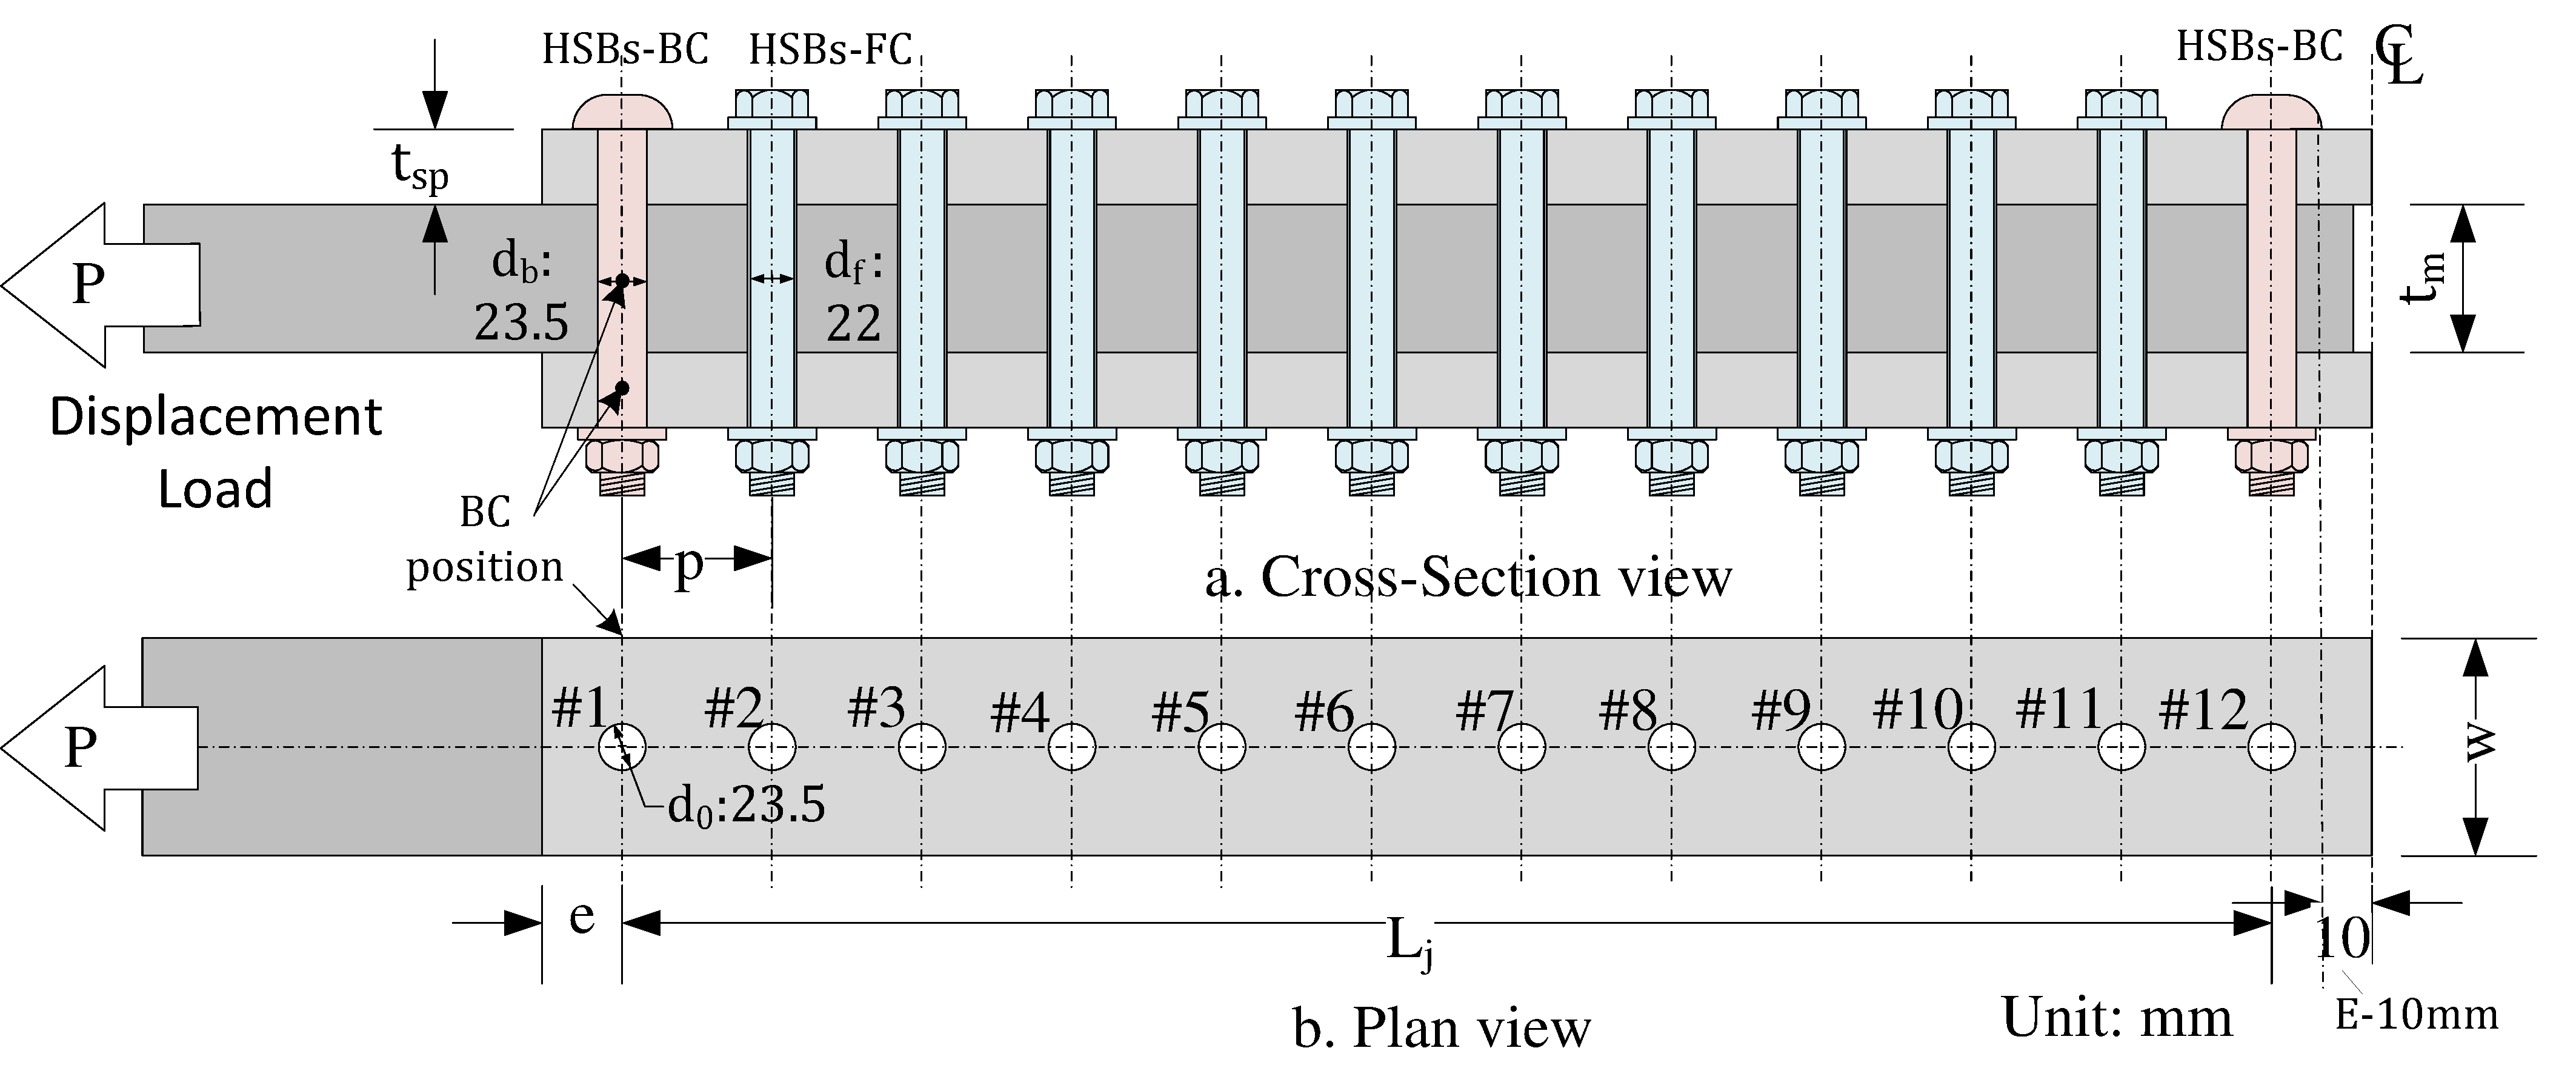
\includegraphics[width=0.95\textwidth]{imgs/ch7/femodelsize.pdf}
    \caption{Schematic illustration of FE model}
    \label{fig-modelsize}
\end{figure*}

\subsection{Modelling methodology}

A general-purpose structural analysis software, Abaqus / Standard 2020, was utilised to perform a three-dimensional finite displacement elastoplastic analysis \cite{Smith2020}. The analytical model was based on a 12-row bolted friction joint as shown in Figure \ref{fig-modelsize}, with the bolt arrangement, joint length, plate thickness and material strength as parameters. Displacement load was applied at the end surface of the main plate, and the analysis was conducted for half of the model, with the centre of the joint in the longitudinal direction set as the axis of symmetry. The diameter of the bearing bolt was set as the same as the bolt hole of 23.5 mm, and the diameter of the friction bolt was set as 22 mm.

The modeling method used in this study is based on the previous research \cite{chen2023mecha}, and the results are compared with the experimental results \cite{chen2024Exp}. The validity of this analysis is provided in Appendix \ref{sec-valid}.

The material properties and nominal stress - nominal strain curves of the materials used in the analysis are presented in Tables \ref{tab-mateproper} and \ref{fig-matpro}. The material SM490Y and SM570 were used for the main plate and splice plates \cite{JISsteel}, and the high-strength bolts of friction and bearing type (hereinafter known as HSB) had material properties of F10T material \cite{JISbolt} (equivalent to ASTM A490 or Grade 10.9) \cite{ASTM-bolt,ISO-bolt}. All material properties were modelled using a trilinear model with a quadratic gradient of $E/100$, and the ultimate strength was considered.

\begin{table*}[!htb]
    \caption{Material properties}
    \label{tab-mateproper}
\begin{tabular}{@{}cccccc@{}}
\toprule
\textbf{Member} &
  \textbf{Material} &
  \textbf{\begin{tabular}[c]{@{}c@{}}Young's modulus\\ {[}$N/mm^2${]}\end{tabular}} &
  \textbf{\begin{tabular}[c]{@{}c@{}}Poisson's ratio\\$v$ \end{tabular}} &
  \textbf{\begin{tabular}[c]{@{}c@{}}Yield strength\\ {[}$N/mm^2${]}\end{tabular}} &
  \textbf{\begin{tabular}[c]{@{}c@{}}Ultimate strength\\ {[}$N/mm^2${]}\end{tabular}} \\ \midrule
\multirow{2}{*}{\begin{tabular}[c]{@{}c@{}}Main plate \\ Splice plate\end{tabular}} &
 SM490Y &  \multirow{3}{*}{200,000} & \multirow{3}{*}{0.3} &  365 &  491 \\
  & SM570 & & & 547 & 635 \\
High-strength bolt &  F10T / B10T & & &  900 &  1091 \\ \bottomrule
\end{tabular}
\end{table*}

\begin{figure}
    \centering
    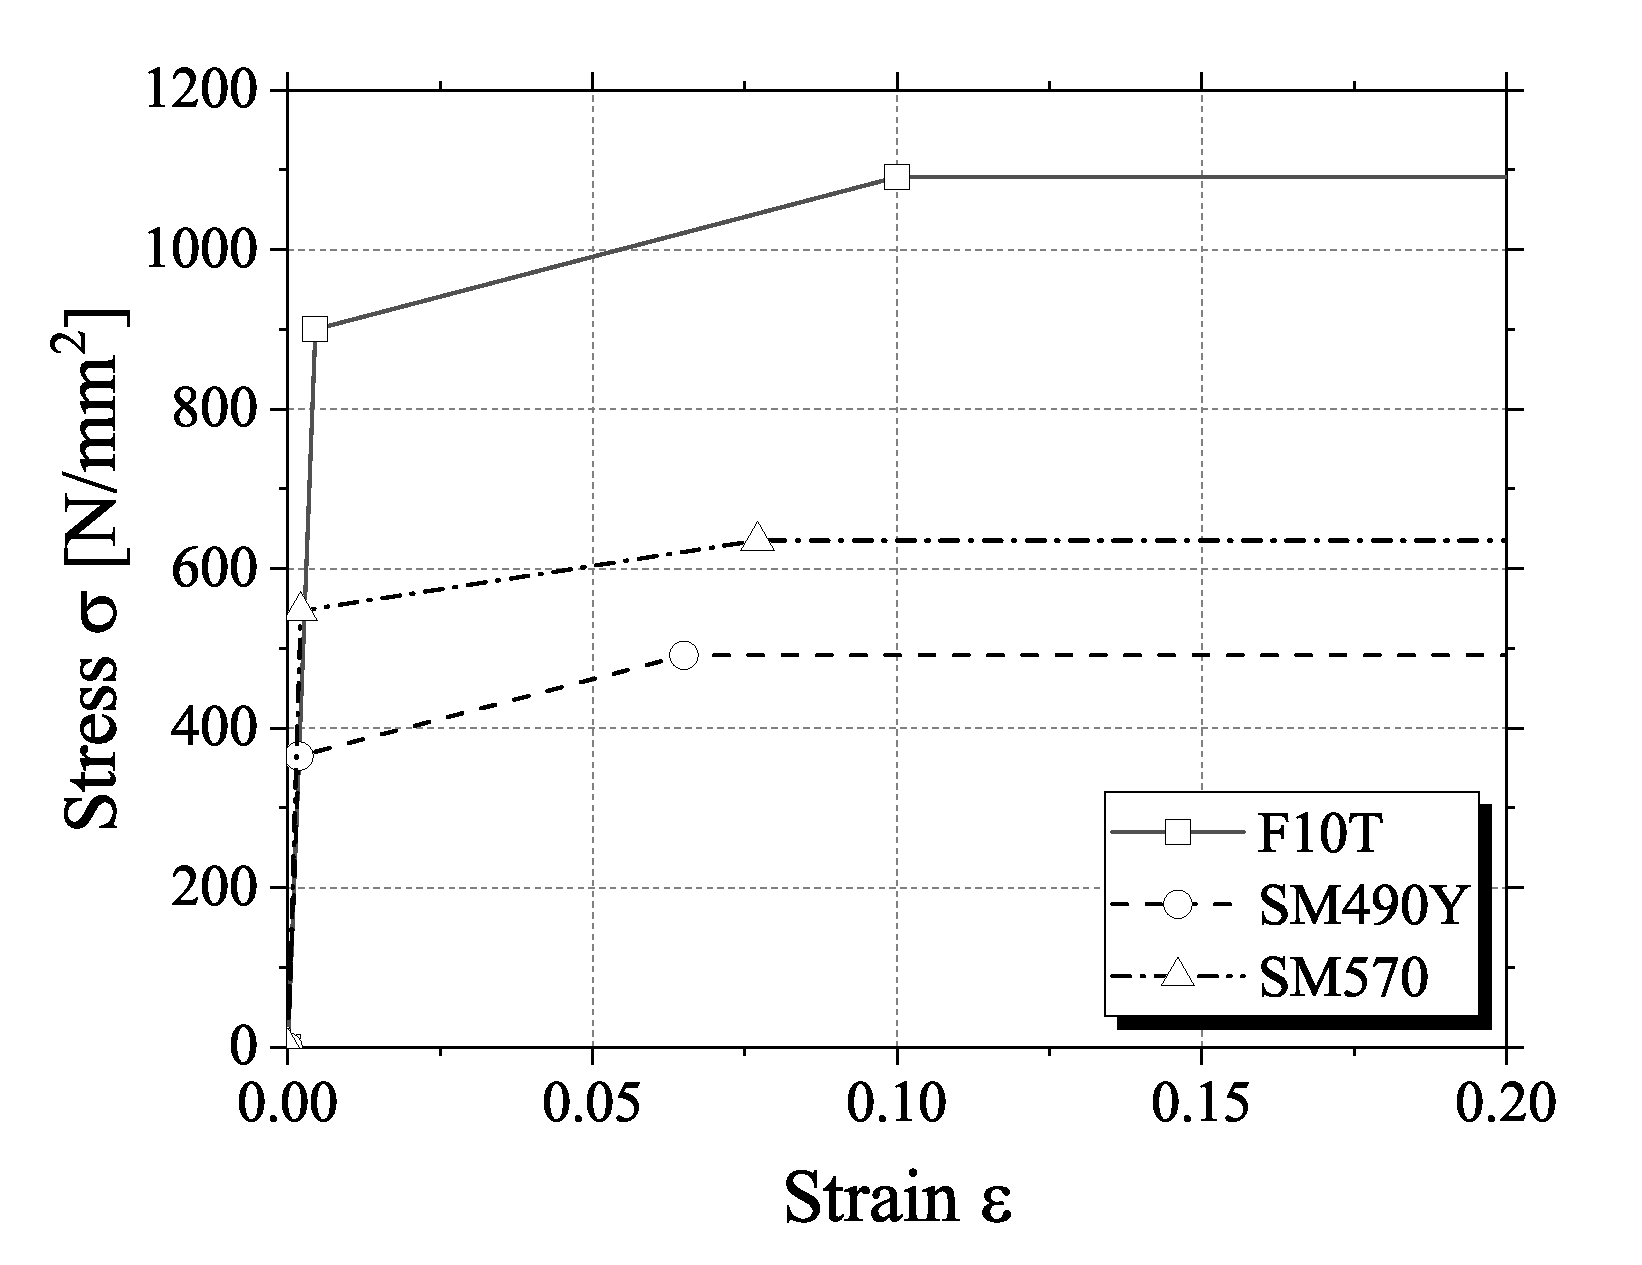
\includegraphics[width=0.6\linewidth]{imgs/ch7/mat-pro.eps}
    \caption{Nominal stress - Nominal strain curves of materials}
    \label{fig-matpro}
\end{figure}

Figure \ref{fig-femesh} depicts the mesh division of the analytical model. The mesh division and element selection are based on the previous study by Ju. S. H. et al. \cite{ju2004-boltfea}. The mesh size for the main plate was set at 1/15 (5 mm) relative to the plate thickness direction. For the friction-type bolt, the mesh size was set to 2 mm, for the bearing-type bolt to 2.9 mm, for the washer to 3 mm, and for the nut to 5 mm. The Incompatible mode eight-node brick element (C3D8I) was utilized in this model, this element utilizes volume integration, allowing for a more accurate representation of large deformations and complex material behaviour.


\begin{figure*}[htbp]
    \centering
    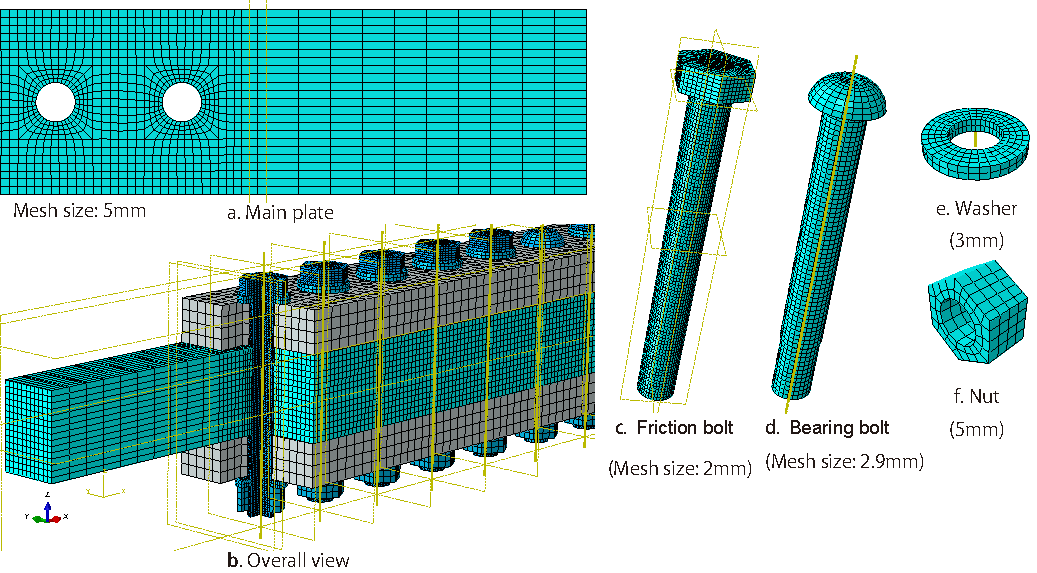
\includegraphics[width=0.95\textwidth]{imgs/ch7/femesh.pdf}
    \caption{FE model mesh division}
    \label{fig-femesh}
\end{figure*}

Contact boundaries were set between the main plate and splice plates, bolt hole wall and bolt shank, and washer and splice plates to simulate the contact conditions, separation, and fixation. For the contact boundary condition (see Figure \ref{fig-contactp}), the surface-to-surface discretization method was used to avoid surface penetration, while the finite sliding tracking approach allowed for unrestricted movement of the contact surfaces. To simulate boundary non-linearity, hard contact and penalty friction were employed to define the normal and tangential behaviours of the contact pairs, with isotropic Coulomb friction modelling the frictional forces. The friction coefficient of this analysis at the faying surface refers the Japanese Specifications for Highway Bridges (JSHB) set at 0.4 \cite{douji2017,shishin2009}. 

The present analysis refers to previous studies \cite{Kim2007,hung1996,Shimozato2008ExperrimentalModel} to modelling the bolt. Initially, the bolt was tightened to the design bolt preload (205 kN) using the Abaqus option for bolt load, and then it was fixed at its original bolt-shank length in subsequent steps. This approach ensures that the bolt length remains constant, allowing the force in the bolt to vary according to the model's response \cite{Smith2020}. In the next step, forced displacement was applied to the end of the main plate.

\begin{figure*}[htbp]
    \centering
    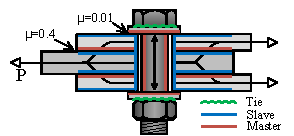
\includegraphics[width=0.5\linewidth]{imgs/ch7/contactp.pdf}
    \caption{Surface definition for contact pairs}
    \label{fig-contactp}
\end{figure*}

\subsection{Analysis case}
To investigate the interaction between friction and bearing in hybrid joints, this study parameterised the arrangement of the bolts, the length of the joint (or number of bolts) and the geometry of the joint, as shown in Table \ref{tab-cases}.

\begin{table}[]
    \centering
\caption{Parameter for FE analysis}
\begin{tabular}{@{}ll@{}}
\toprule
Parameter                   &              \\ \midrule
Number of Row               & 8, 10, 12      \\
Number of Fit bolt          & 0, 2, 4, 6, 8, 12 \\
Material property {[}Mpa{]} & 365, 547     \\
Bolt peach [mm]             & 75, 80, 85     \\
End distance  [mm]          & 35, 40, 50     \\ \bottomrule
\end{tabular}
\label{tab-cases}
\end{table}

\subsection{Calculation of joint resistance}

\begin{table*}[htbp]
\centering
\caption{Detail of analysis case}
\begin{tabular}{@{}llllllllllllllll@{}}
\toprule
code & $w$ & $t_m$ & $t_{sp}$ & $n$ & $n_b$ & $p$ & $e$ & $L_j$ & $f_y$ & $F_s$ & $F_b$ & $F_{h,sh}$ & $F_y$ & $\beta_1$ & $\beta_h$ \\ \midrule
OA0 & 110 & 75 & 38 & 12 & 0 & 75 & 40 & 825 & 365 & 1968 & - & - & 2368 & 0.83 & - \\
OA2 & 110 & 75 & 38 & 12 & 2 & 75 & 40 & 825 & 365 & 1968 & 902 & 2870 & 2368 & 0.83 & 1.23 \\
OA4 & 110 & 75 & 38 & 12 & 4 & 75 & 40 & 825 & 365 & 1968 & 1803 & 3771 & 2368 & 0.83 & 1.6 \\
OA12 & 110 & 75 & 38 & 12 & 12 & 75 & 40 & 825 & 365 & 1968 & 5412 & 5412 & 2368 & 0.83 & 2.28 \\
OAP0 & 110 & 75 & 38 & 12 & 0 & 80 & 50 & 880 & 365 & 1968 & - & - & 2368 & 0.83 & - \\
OAP2 & 110 & 75 & 38 & 12 & 2 & 80 & 50 & 880 & 365 & 1968 & 902 & 2870 & 2368 & 0.83 & 1.23 \\
OAP4 & 110 & 75 & 38 & 12 & 4 & 80 & 50 & 880 & 365 & 1968 & 1803 & 3771 & 2368 & 0.83 & 1.6 \\
OAK0 & 110 & 75 & 38 & 12 & 0 & 80 & 50 & 880 & 365 & 1968 & - & - & 2368 & 0.83 & - \\
OAK2 & 110 & 75 & 38 & 12 & 2 & 80 & 50 & 880 & 365 & 1968 & 902 & 2870 & 2368 & 0.83 & 1.23 \\
OAK4 & 110 & 75 & 38 & 12 & 4 & 80 & 50 & 880 & 365 & 1968 & 1803 & 3771 & 2368 & 0.83 & 1.6 \\
OA2B & 110 & 75 & 38 & 12 & 2 & 75 & 40 & 825 & 547 & 1968 & 902 & 2870 & 3548 & 0.55 & 0.81 \\
OA4B & 110 & 75 & 38 & 12 & 4 & 75 & 40 & 825 & 547 & 1968 & 1803 & 3771 & 3548 & 0.55 & 1.06 \\
OAP2B & 110 & 75 & 38 & 12 & 2 & 80 & 50 & 825 & 547 & 1968 & 902 & 2870 & 3548 & 0.55 & 0.81 \\
OAP4B & 110 & 75 & 38 & 12 & 4 & 80 & 50 & 825 & 547 & 1968 & 1803 & 3771 & 3548 & 0.55 & 1.06 \\
OAK2B & 110 & 75 & 38 & 12 & 2 & 85 & 50 & 825 & 547 & 1968 & 902 & 2870 & 3548 & 0.55 & 0.81 \\
OAK4B & 110 & 75 & 38 & 12 & 4 & 85 & 50 & 825 & 547 & 1968 & 1803 & 3771 & 3548 & 0.55 & 1.06 \\
KA0 & 110 & 75 & 38 & 10 & 0 & 75 & 40 & 675 & 365 & 1640 & - & - & 2368 & 0.69 & - \\
KA2 & 110 & 75 & 38 & 10 & 2 & 75 & 40 & 675 & 365 & 1640 & 902 & 2542 & 2368 & 0.69 & 1.07 \\
KA4 & 110 & 75 & 38 & 10 & 4 & 75 & 40 & 675 & 365 & 1640 & 1803 & 3443 & 2368 & 0.69 & 1.46 \\
KAP2 & 110 & 75 & 38 & 10 & 2 & 80 & 50 & 720 & 365 & 1640 & 902 & 2542 & 2368 & 0.69 & 1.07 \\
KAP4 & 110 & 75 & 38 & 10 & 4 & 80 & 50 & 720 & 365 & 1640 & 1803 & 3443 & 2368 & 0.69 & 1.46 \\
KAK2 & 110 & 75 & 38 & 10 & 2 & 85 & 50 & 765 & 365 & 1640 & 902 & 2542 & 2368 & 0.69 & 1.07 \\
KAK4 & 110 & 75 & 38 & 10 & 4 & 85 & 50 & 765 & 365 & 1640 & 1803 & 3443 & 2368 & 0.69 & 1.46 \\
KA2B & 110 & 75 & 38 & 10 & 2 & 75 & 40 & 675 & 547 & 1640 & 902 & 2542 & 3548 & 0.46 & 0.71 \\
KA4B & 110 & 75 & 38 & 10 & 4 & 75 & 40 & 675 & 547 & 1640 & 1803 & 3443 & 3548 & 0.46 & 0.97 \\
KAK2B & 110 & 75 & 38 & 10 & 2 & 80 & 50 & 720 & 547 & 1640 & 902 & 2542 & 3548 & 0.46 & 0.71 \\
KAK4B & 110 & 75 & 38 & 10 & 4 & 80 & 50 & 720 & 547 & 1640 & 1803 & 3443 & 3548 & 0.46 & 0.97 \\
KAP2B & 110 & 75 & 38 & 10 & 2 & 85 & 50 & 765 & 547 & 1640 & 902 & 2542 & 3548 & 0.46 & 0.71 \\
KAP4B & 110 & 75 & 38 & 10 & 4 & 85 & 50 & 765 & 547 & 1640 & 1803 & 3443 & 3548 & 0.46 & 0.97 \\
HA2 & 110 & 75 & 38 & 8 & 2 & 75 & 40 & 525 & 365 & 1312 & 902 & 2214 & 2368 & 0.55 & 0.94 \\
HA4 & 110 & 75 & 38 & 8 & 4 & 75 & 40 & 525 & 365 & 1312 & 1803 & 3115 & 2368 & 0.55 & 1.3 \\
HAP2 & 110 & 75 & 38 & 8 & 2 & 80 & 50 & 560 & 365 & 1312 & 902 & 2214 & 2368 & 0.55 & 0.94 \\
HAP4 & 110 & 75 & 38 & 8 & 4 & 80 & 50 & 560 & 365 & 1312 & 1803 & 3115 & 2368 & 0.55 & 1.3 \\
HAK2 & 110 & 75 & 38 & 8 & 2 & 85 & 50 & 595 & 365 & 1312 & 902 & 2214 & 2368 & 0.55 & 0.94 \\
HAK4 & 110 & 75 & 38 & 8 & 4 & 85 & 50 & 595 & 365 & 1312 & 1803 & 3115 & 2368 & 0.55 & 1.3 \\
HA2B & 110 & 75 & 38 & 8 & 2 & 75 & 40 & 525 & 547 & 1312 & 902 & 2214 & 3548 & 0.37 & 0.62 \\
HA4B & 110 & 75 & 38 & 8 & 4 & 75 & 40 & 525 & 547 & 1312 & 902 & 3115 & 3548 & 0.37 & 0.88 \\
HAP2B & 110 & 75 & 38 & 8 & 2 & 80 & 50 & 560 & 547 & 1312 & 902 & 2214 & 3548 & 0.37 & 0.62 \\
HAP4B & 110 & 75 & 38 & 8 & 4 & 80 & 50 & 560 & 547 & 1312 & 902 & 3115 & 3548 & 0.37 & 0.88 \\
HAK2B & 110 & 75 & 38 & 8 & 2 & 85 & 50 & 595 & 547 & 1312 & 902 & 2214 & 3548 & 0.37 & 0.62 \\
HAK4B & 110 & 75 & 38 & 8 & 4 & 85 & 50 & 595 & 547 & 1312 & 902 & 3115 & 3548 & 0.37 & 0.88 \\
W2B-M16 & 210 & 50 & 28 & 10 & 2 & 55 & 35 & 495 & 547 & 848 & 418 & 1265 & 5251 & 0.16 & 0.24 \\
W2B-t30 & 210 & 30 & 28 & 10 & 2 & 55 & 35 & 495 & 547 & 848 & 418 & 1265 & 3151 & 0.27 & 0.4 \\
W4B & 210 & 50 & 28 & 10 & 4 & 55 & 35 & 495 & 547 & 848 & 836 & 1684 & 5251 & 0.16 & 0.32 \\
W6B & 210 & 50 & 28 & 10 & 6 & 55 & 35 & 495 & 547 & 848 & 1254 & 2102 & 5251 & 0.16 & 0.4 \\ \bottomrule
\end{tabular}
\label{tab-allcase}
\end{table*}

The design strengths of all cases are presented in Table \ref{tab-allcase}. To investigate the load-sharing state and mechanical behaviour of a single bolt, the resistance (slip, bearing, and shear resistance) per bolt was calculated using Eqs. (\ref{eq-fds1}–\ref{eq-fdsy1}). The design strength of the entire bolted joint was calculated using Eqs. (\ref{eq-fdy}–\ref{eq-fdsy}). 

Since this study considers that the hybrid connection will not exhibit significant slip, the reduction factor for the friction force based on the joint length specified in JSHB \cite{douji2017} is not taken into account.

\noindent Slip resistance per a fastener $F_{s1}$:
\begin{equation}
    \label{eq-fds1}
    F_{s1} = \mu \times N_d \times m
\end{equation}

\noindent Total slip resistance of the joint $F_{s}$:
\begin{equation}
    \label{eq-fds}
    F_{s} = (n_f+n_b) \times F_{s1}
\end{equation}

For the bearing resistance of the bolt hole, although the JSHB follows the formula $1. 7f_y$ for the design of ASD methods, this formula is too high for the evaluation of (Serviceability Limit States) SLS, especially for the hybrid connection, the bearing bolt always has to share more force than the general friction bolts, so for the design of bearing resistance for the hybrid connection, the previous study concludes \cite{chen2023mecha} that it is more reliable to cancel the factor before the yield strength part, and the design formula for bearing yield resistance for a fastener $F_{by1}$ is as follows:

\begin{equation}
    \label{eq-fdb1}
    F_{by1} = \sigma_y \times t \times d_b
\end{equation}

Bolt-shank shear yield resistance per fastener $F_{shy1}$:
\begin{equation}
    \label{eq-fdsy1}
    F_{shy1} = \sigma_{yb} / \sqrt{3} \times 2 \pi \times (0.5d_b)^2
\end{equation}

Net cross-sectional yield strength of the plate $F_y$:
\begin{equation}
    \label{eq-fdy}
    F_{y} = (w-d_0)t \times \sigma_y
\end{equation}

Ultimate tensile strength of the plate $F_u$ :
\begin{equation}
    \label{eq-fdu}
    F_{u} = (w-d_0)t \times \sigma_u
\end{equation}

Bolt shank shear yield resistance (total) $F_{shy}$ :
\begin{equation}
    \label{eq-fdsy}
    F_{shy} = F_{shy1} \times n_b
\end{equation}

Bearing resistance for bolt hole $F_{by}$ :
\begin{equation}
    F_{by} = d_0 t \times \sigma_{y} \times n_b
\end{equation}

Bearing resistance of fit bolt $F_b$:
\begin{equation}
    F_b = min(F_{shy}, F_{by})
\end{equation}

For hybrid joint, the joint resistance $F_{h}$ \cite{chen2023mecha} is:
\begin{equation} \label{eq-fh}
\begin{aligned}
    F_{h,b} &= (n_f+n_b) F_{s1} + n_b F_{by1} \\
    F_{h,sh} &= (n_f+n_b) F_{s1} + n_b F_{shy1} \\
    F_{h} &= min(F_{h,b}, F_{h,sh})
\end{aligned}    
\end{equation}

Where,

\begin{tabular}{ll}
$\sigma_y$ & the yield strengths of the main plate; \\
$\sigma_u$ & the ultimate strengths of the main plate;\\
$\sigma_{yb}$ & the yield strength of the HSB; \\ 
$\mu$ & the friction coefficient;\\ 
$t$ & the thickness of the main plate; \\ 
$w$ & the width of the main plate; \\
$d_0$ & the hole diameter; \\ 
$d_b$ & the diameter of the bolt; \\ 
$N_0$ & Bolt preload before loading; \\
$N_d$ & the design bolt preload; \\
$m$ & the number of shear planes; \\ 
$n_{f}$ & the number of friction-type bolts; \\ 
$n_b$ & the number of bearing-type bolts.
\end{tabular}


\section{Validation of FE model}
\label{sec-valid}


\begin{figure*}
    \centering
    \begin{subfigure}[b]{0.48\linewidth}
        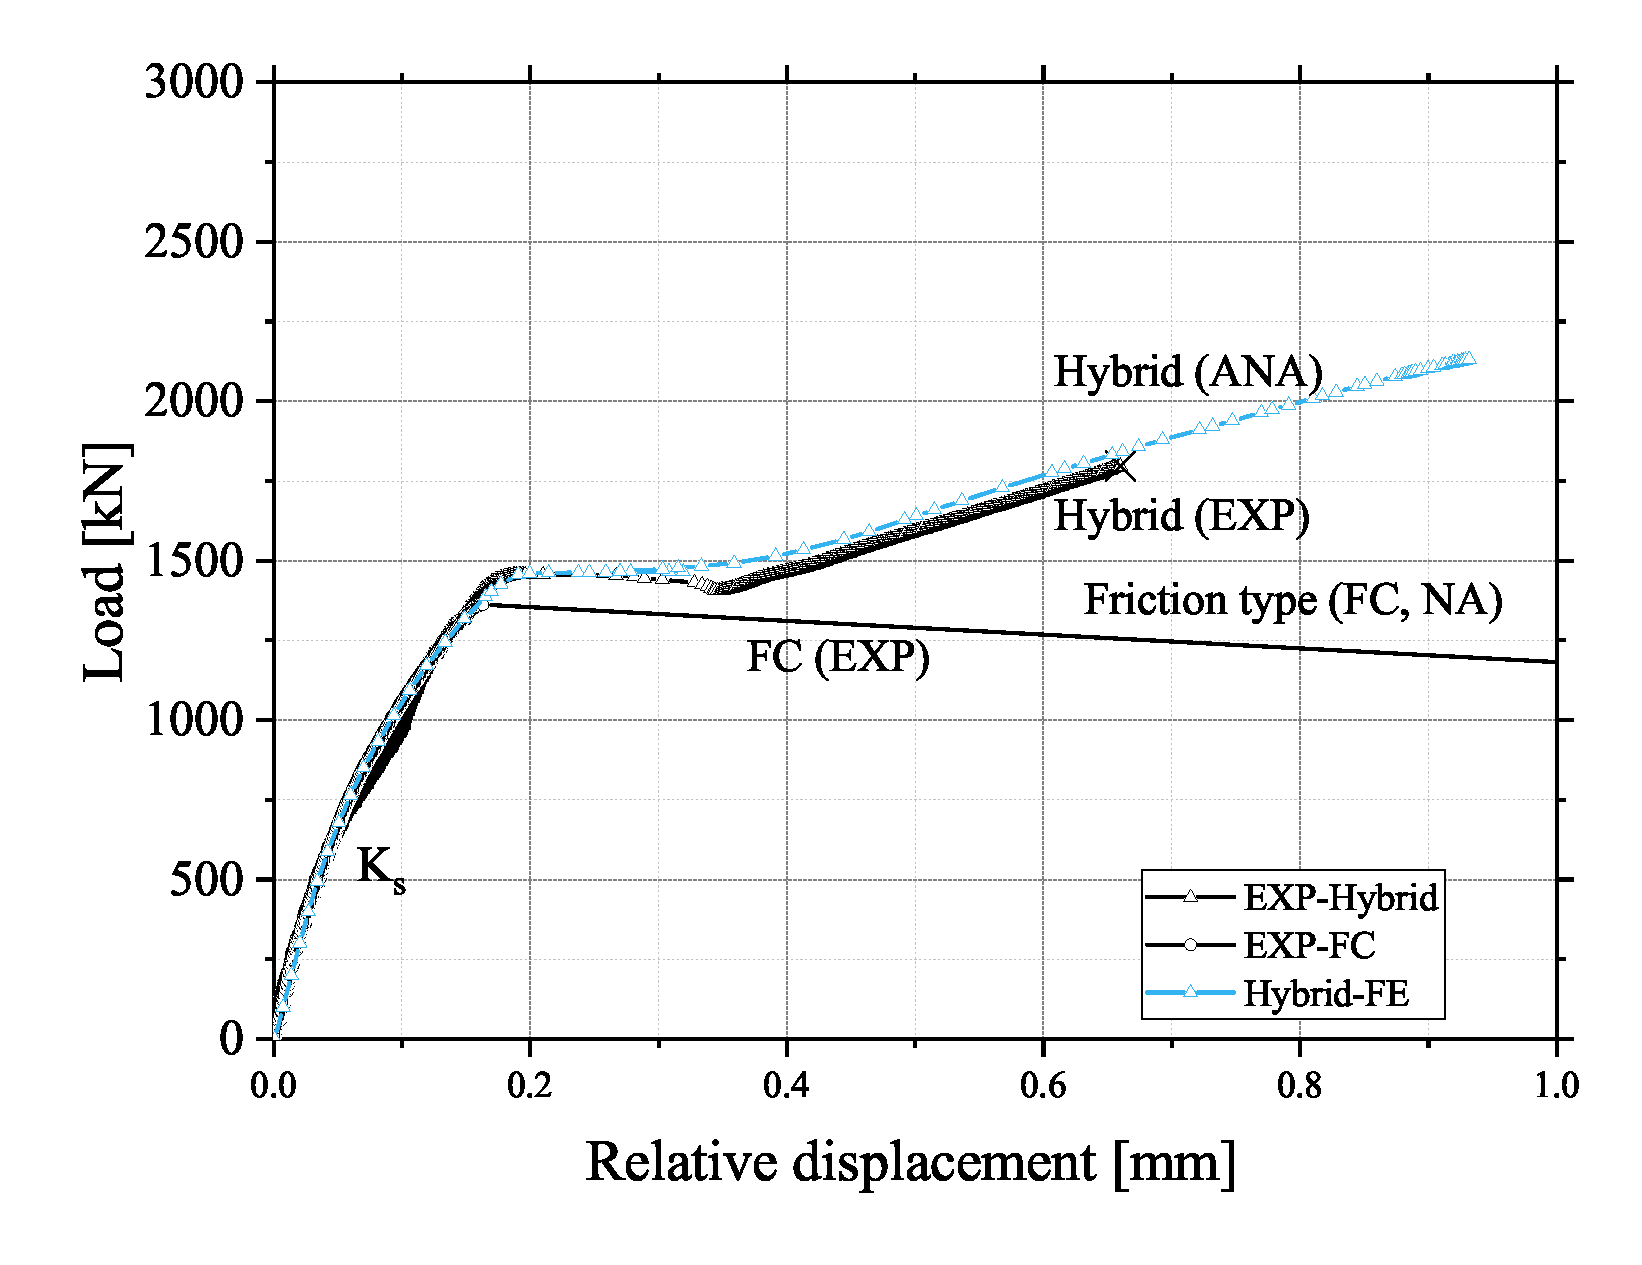
\includegraphics[width=\linewidth]{imgs/ch7/valid-rd.eps}
        \caption{The relationship between load and relative displacement of FE analysis and Experiment result}
        \label{fig-valid-rd}
    \end{subfigure}
    \hfill
    \begin{subfigure}[b]{0.48\linewidth}
    \centering
        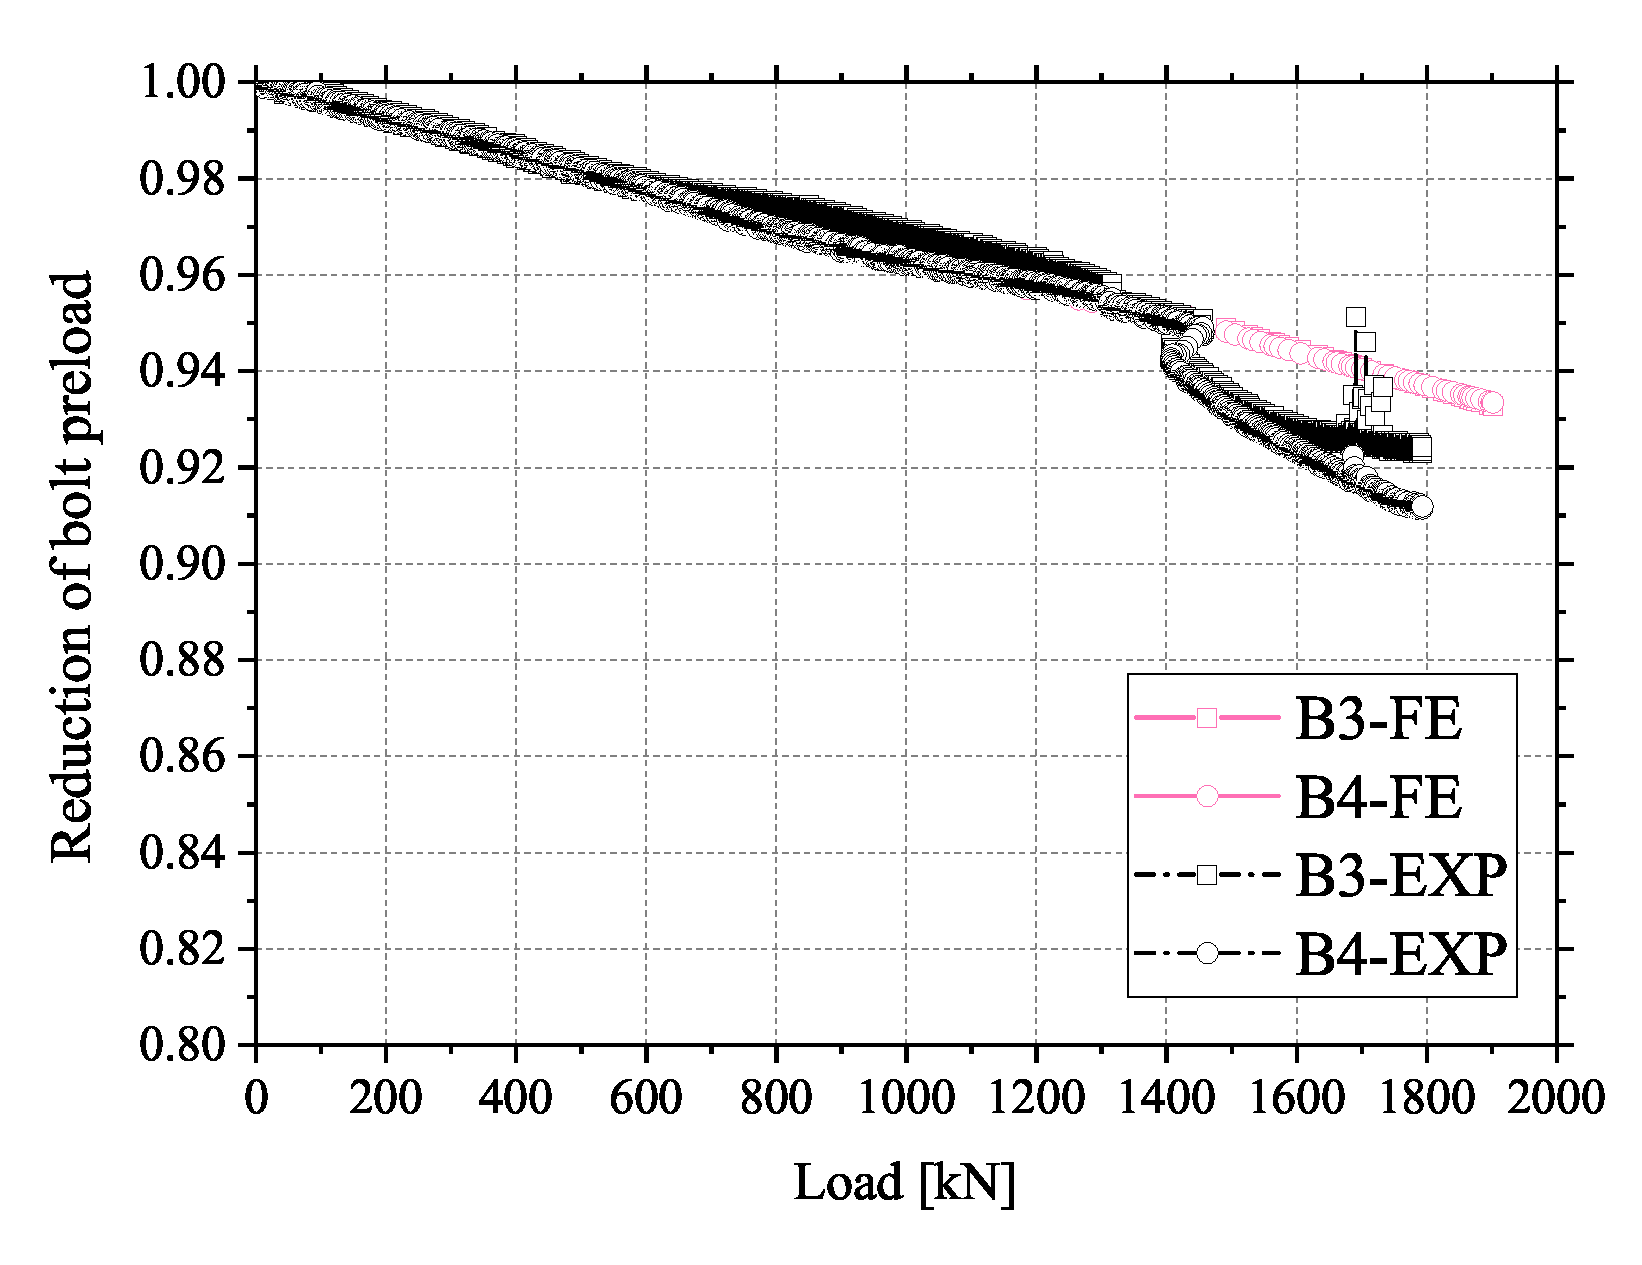
\includegraphics[width=\linewidth]{imgs/ch7/valid-boltAF.eps}
        \caption{The relationship between reduction of bolt preload and load}
        \label{fig-valid-redc}
    \end{subfigure}
    
    \caption{Compare with FE analysis result and experiment result \cite{chen2024Exp} }
    \label{fig-valid}
\end{figure*}

The FE analysis model in this paper refers to the Previous study by CHEN et, al. \cite{chen2023mecha} and uses the same modelling method. Additionally, Figure \ref{fig-valid-rd} shows the tensile test results of a full-scale hybrid connection \cite{chen2024Exp} and the analysis results of the FE model used in this paper. The blue triangles represent the analytical results, and the black triangles represent the experimental results from previous research. It can be observed that the FE analysis results match well with the experimental results. Figure \ref{fig-valid-redc} shows the bolt preload reduction rates of bolts \# 3 and \# 4 used for friction connection. The pink colour represents the analytical results, and the black colour represents the experimental results measured by the strain gauge. It can be seen that the bolt preload reduction rates in the analysis and experiment results are almost the same. Furthermore, at 1400 kN, the experimental results exhibit a more noticeable change, and the slope of the curve also changes after this point. This is because, in the experiment, due to the failure of friction, the connection experienced a significant slip (the bolts were subjected to a large impact due to the slip), while the analysis is based on static simulation and does not exhibit such dynamic behaviour. Therefore, the load reduction of the bolt axial force appears more gradual in the analysis. It could be considered this analysis method is validity. 

\section{Analysis Result and Discussion}



\subsection{Deformation of hybrid connection}

Figure \ref{fig-ldef} shows the relationship between load and deformation. The deformation of the joint is obtained from the average displacement of the cross-section at the end of the joint. The OA0 case represents the friction type connection (hereafter known as the FC), OA12 represents the bearing type connection ((hereafter known as the BC)) with 12 fitted bolts, and OA2, 2B and 4B represent the hybrid connections. It can be seen from the figure that regardless of the type of connection, their initial stiffness is the same because the initial stiffness is mainly determined by the friction. When the friction connection experiences major slippage, the deformation of the connection is 1.17 mm, while for the hybrid connection (see OA2B), when the bolt shank shear yielding $P_{h,sh}$ occurs, the deformation of the connection is 1.51 mm. The difference is only 0.34 mm. Additionally, after the hybrid connection reaches bolt shank shear yielding, the slope of the curve decreases until all bolts enter the bearing. It can be observed that after the connection is configured with fitted bolts, the strength of the connection is significantly increased, and it exhibits a curve variation similar to the friction connection.

Where the bolt shank shear yielding $P_{hv}$ represents the shear yielding resistance of any of the fit bolt's shank in the analysis. As shown in Figure \ref{fig-bsh-jud-peeq}, the definition of bolt shank shear yield (SLS) is when an equivalent plastic strain (PEEQ) greater than 0.001 occurs throughout the shear plane.

\begin{figure}
    \centering
    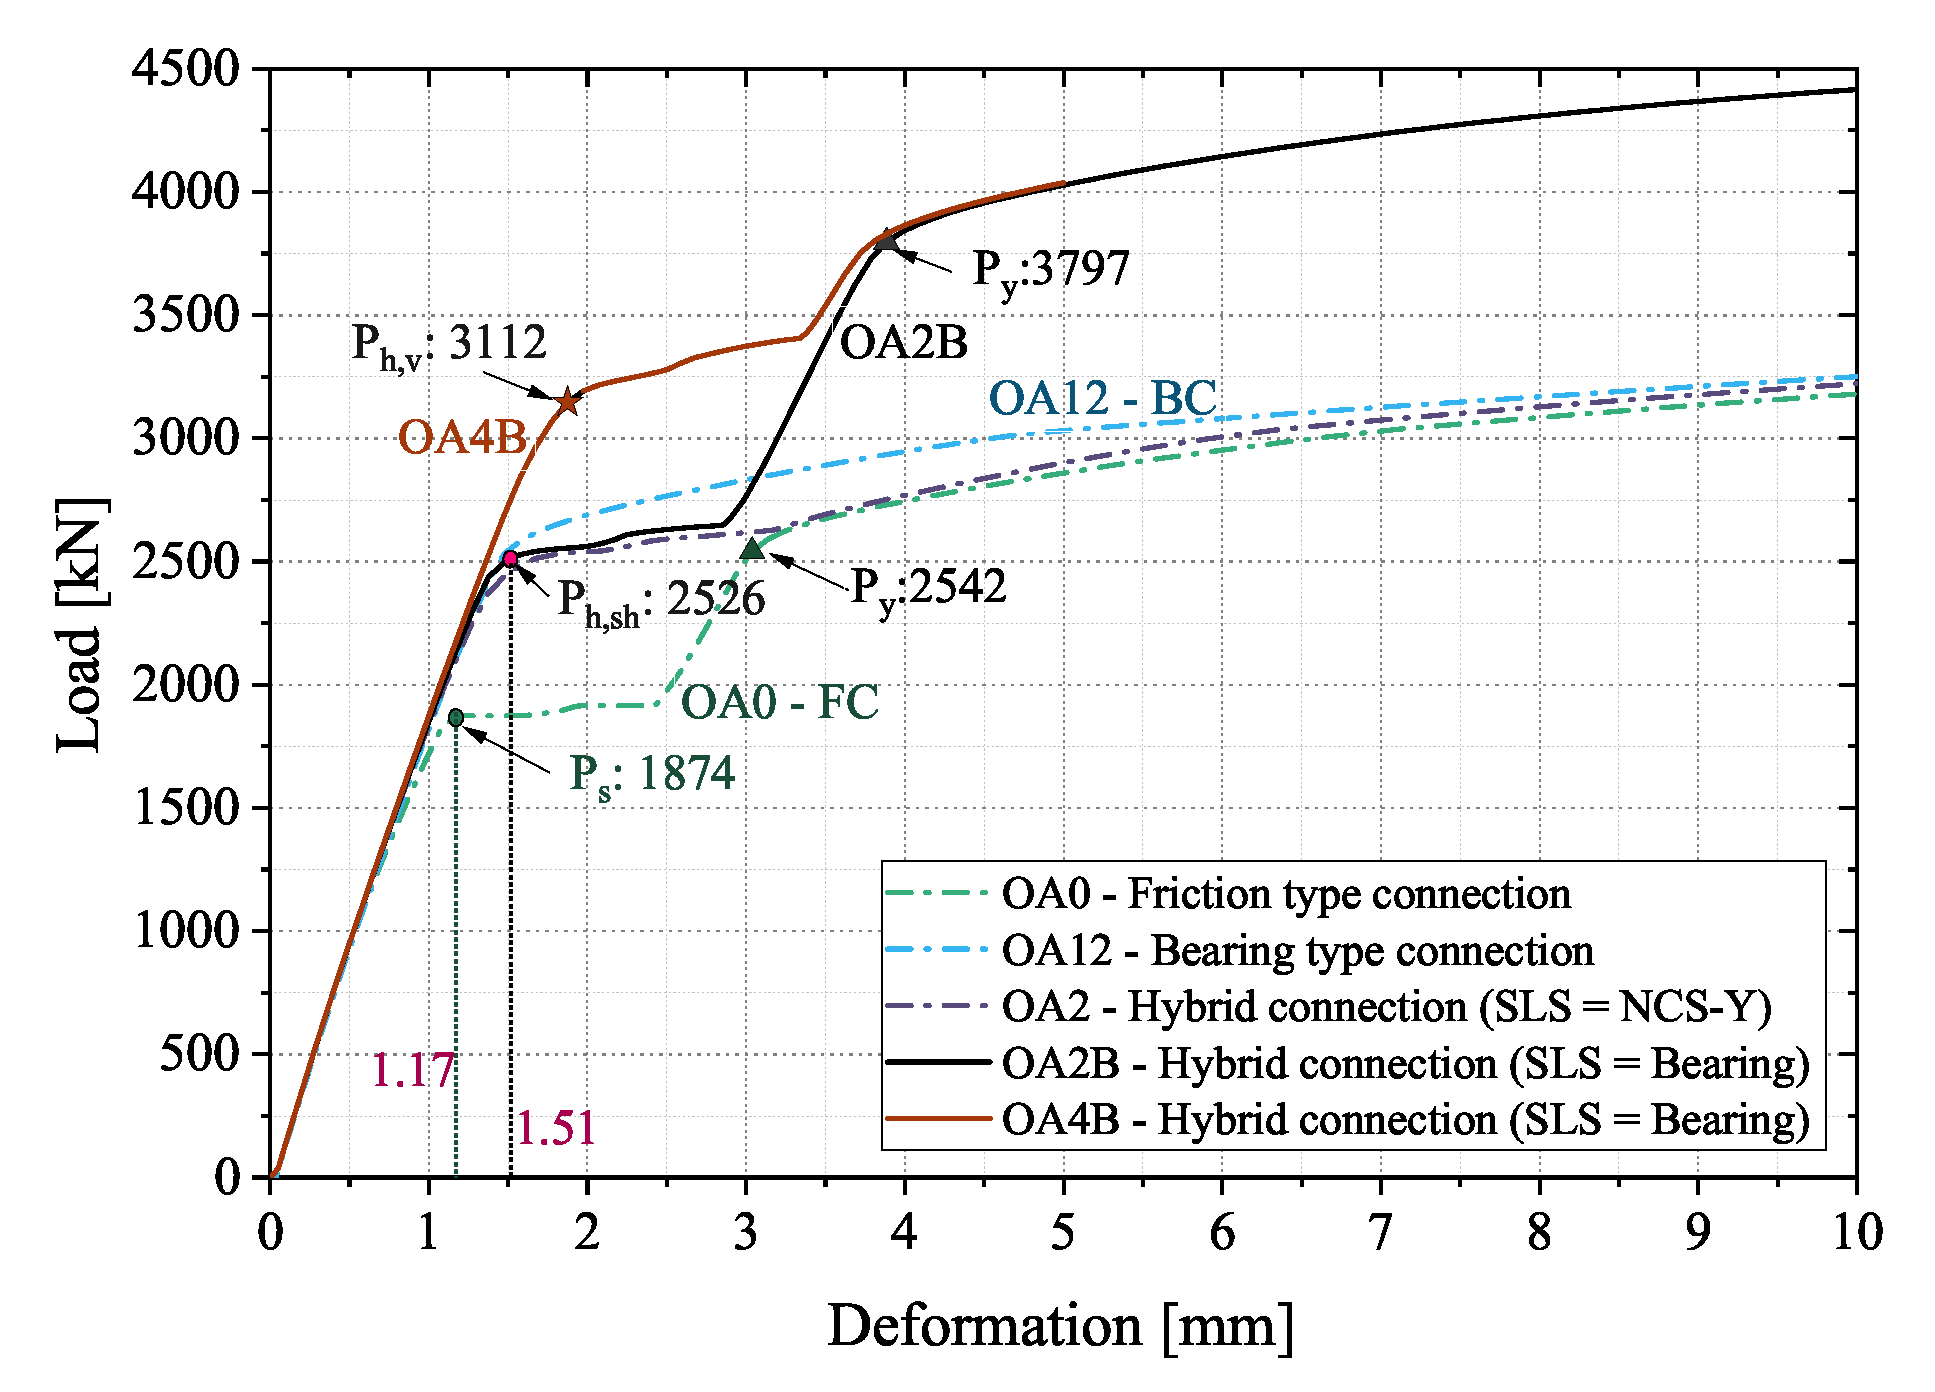
\includegraphics[width=\linewidth]{imgs/ch7/LDef-total.eps}
    \caption{The relationship between load and deformation}
    \label{fig-ldef}
\end{figure}

\begin{figure}
    \centering
    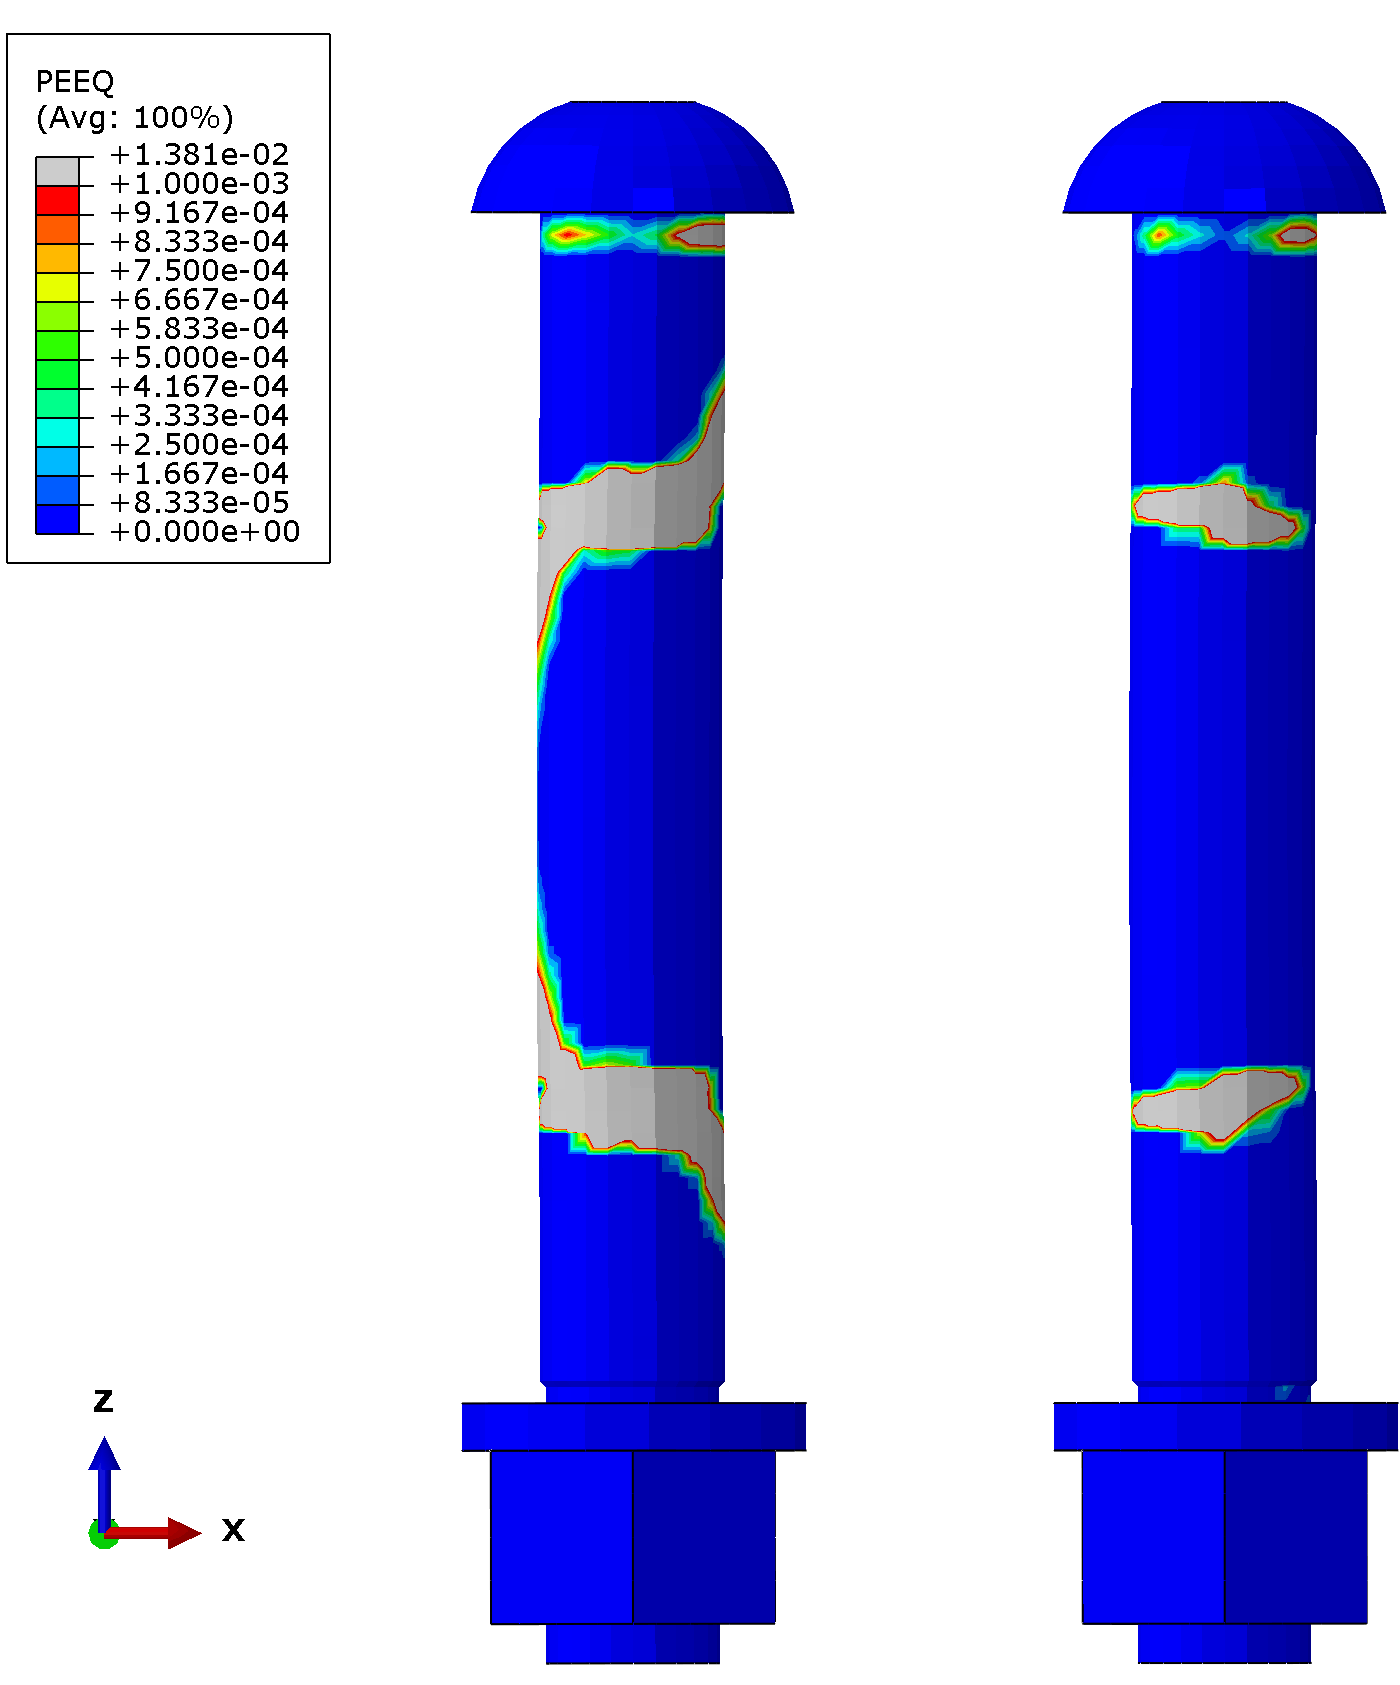
\includegraphics[width=0.6\linewidth]{imgs/ch7/bsh-jud-peeq.png}
    \caption{Judgement of bolt shear yield load $P_{h,sh}$. (PEEQ counter)}
    \label{fig-bsh-jud-peeq}
\end{figure}

\subsection{Divide the load into bearing and frictional forces}


\begin{figure*}
\centering
% \begin{subfigure}[b]{0.7\textwidth}
%     \centering
%     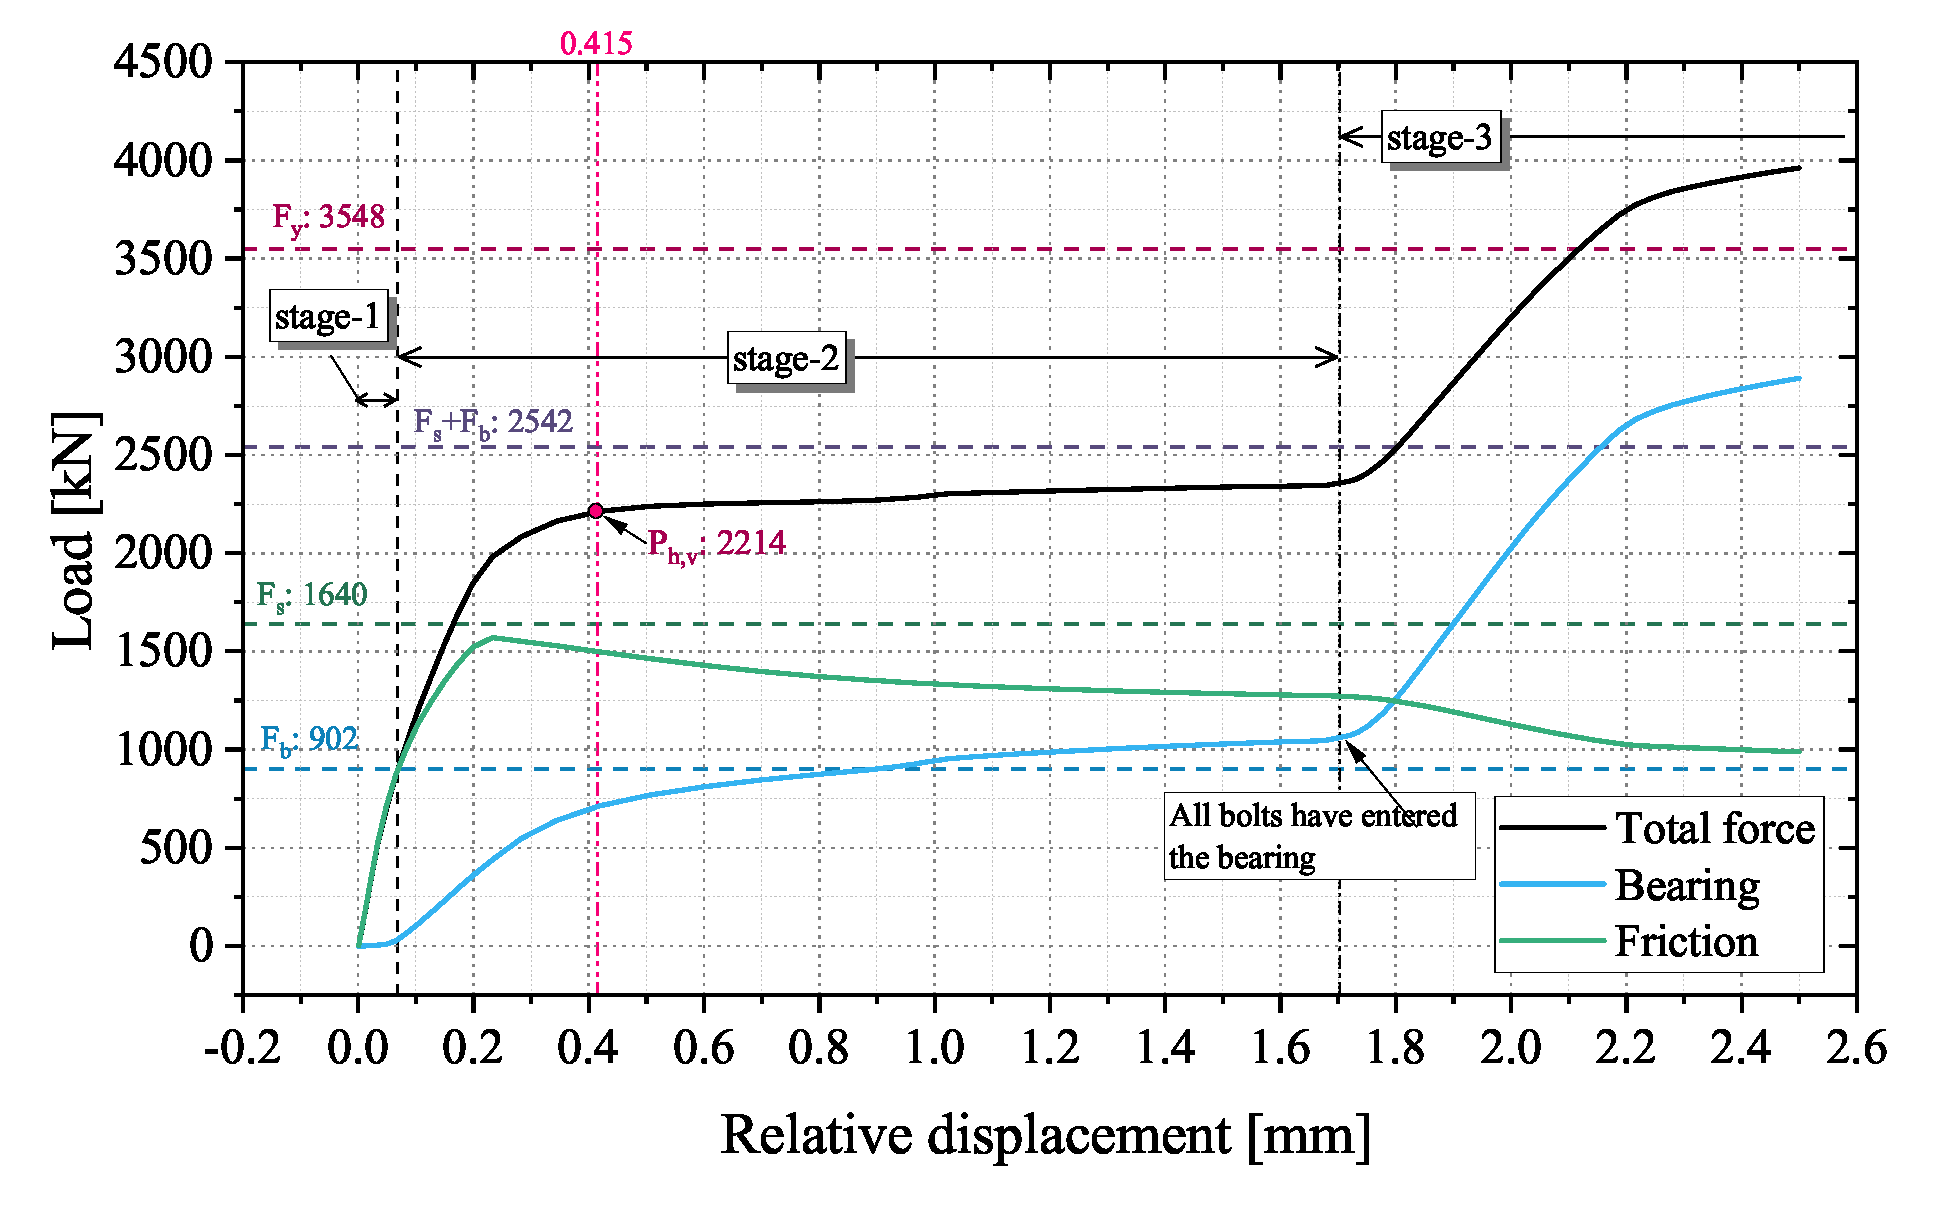
\includegraphics[width=\textwidth]{imgs/ch7/LD-KA2B.eps}
%     \caption{KA2B case}
%     \label{fig-ldka2b}
% \end{subfigure}
% \hfill
% \begin{subfigure}[b]{0.7\textwidth}
%     \centering
%     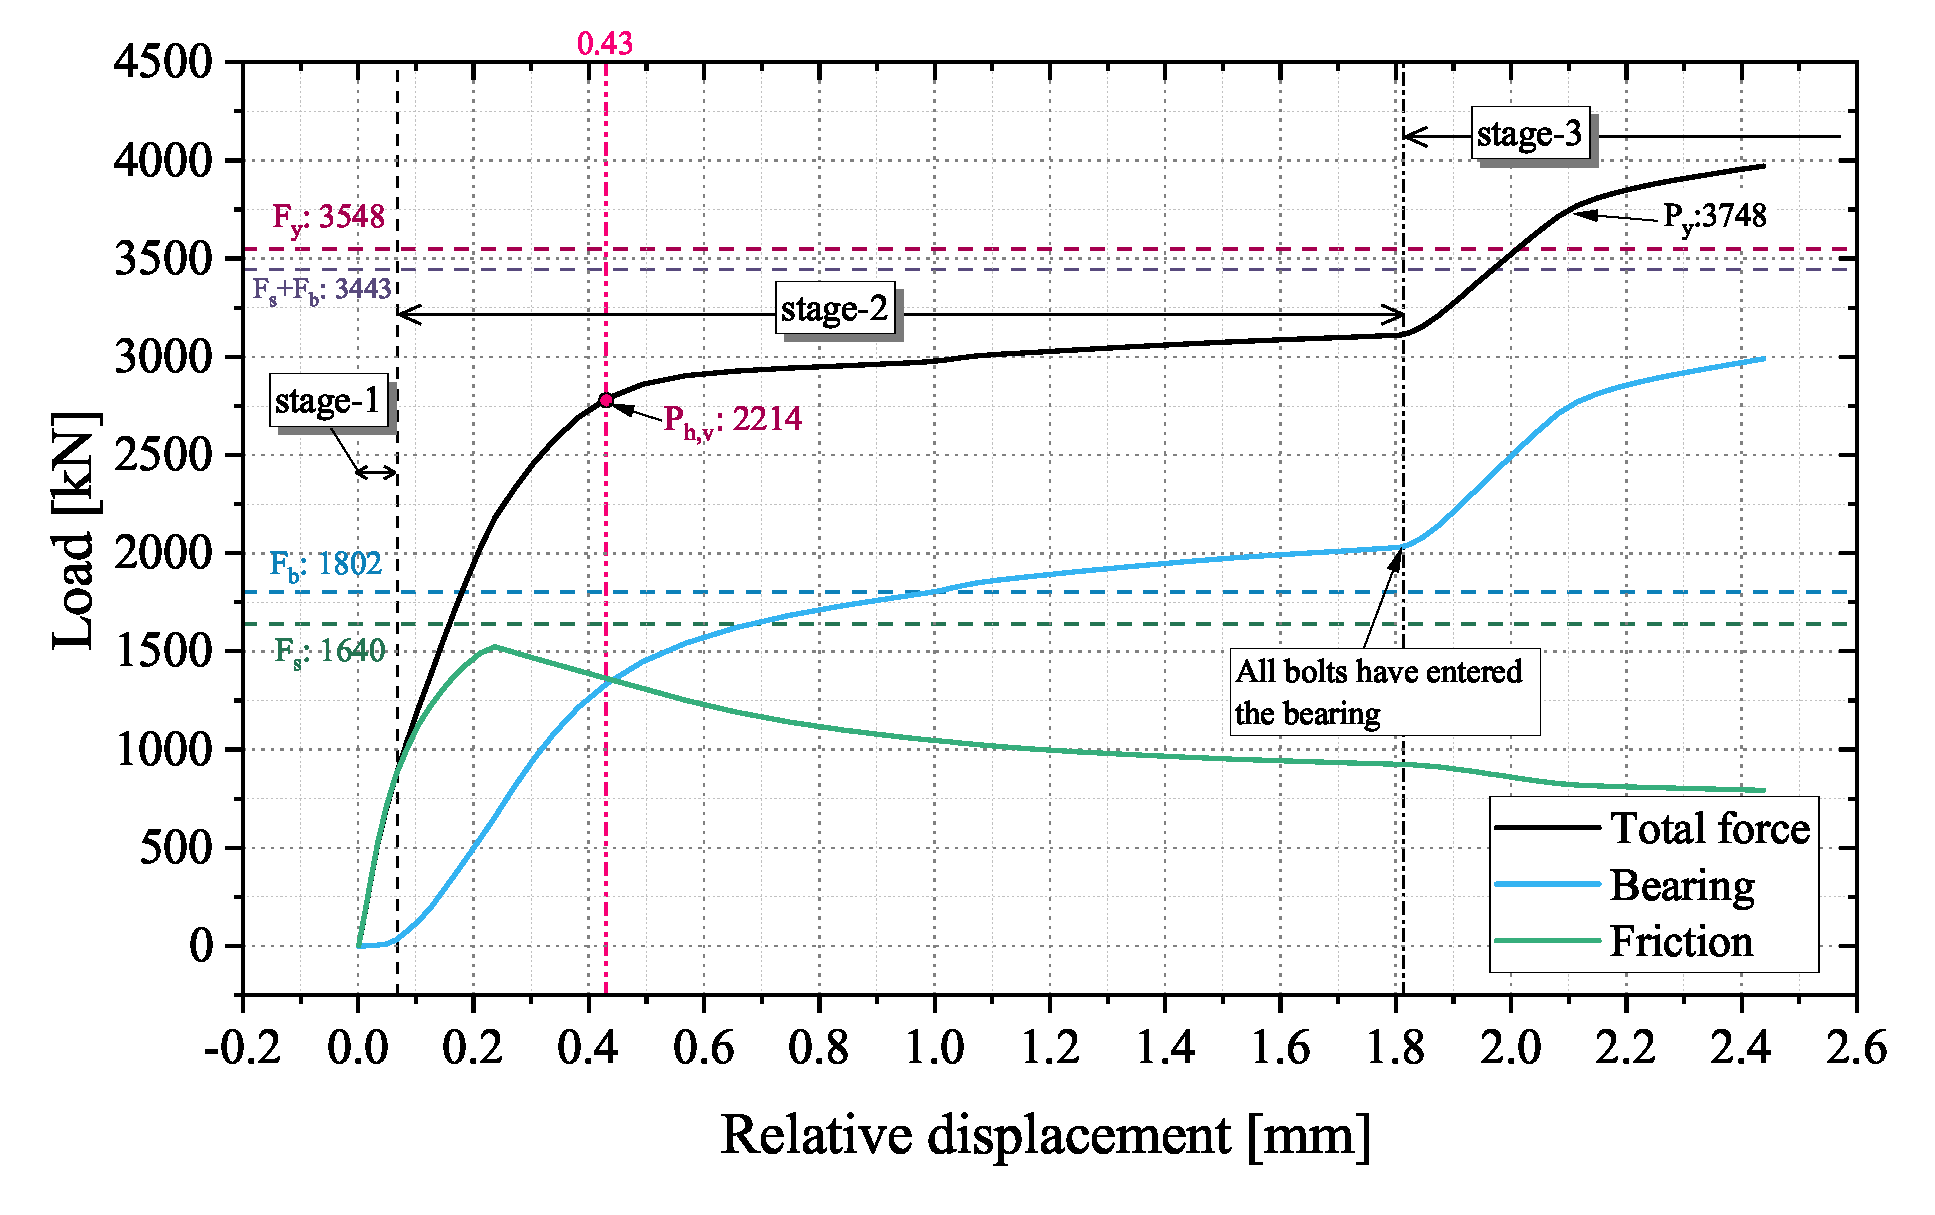
\includegraphics[width=\textwidth]{imgs/ch7/LD-KA4B.eps}
%     \caption{KA4B case}
%     \label{fig-ldka4b}
% \end{subfigure}

\begin{subfigure}[b]{0.9\textwidth}
    \centering
    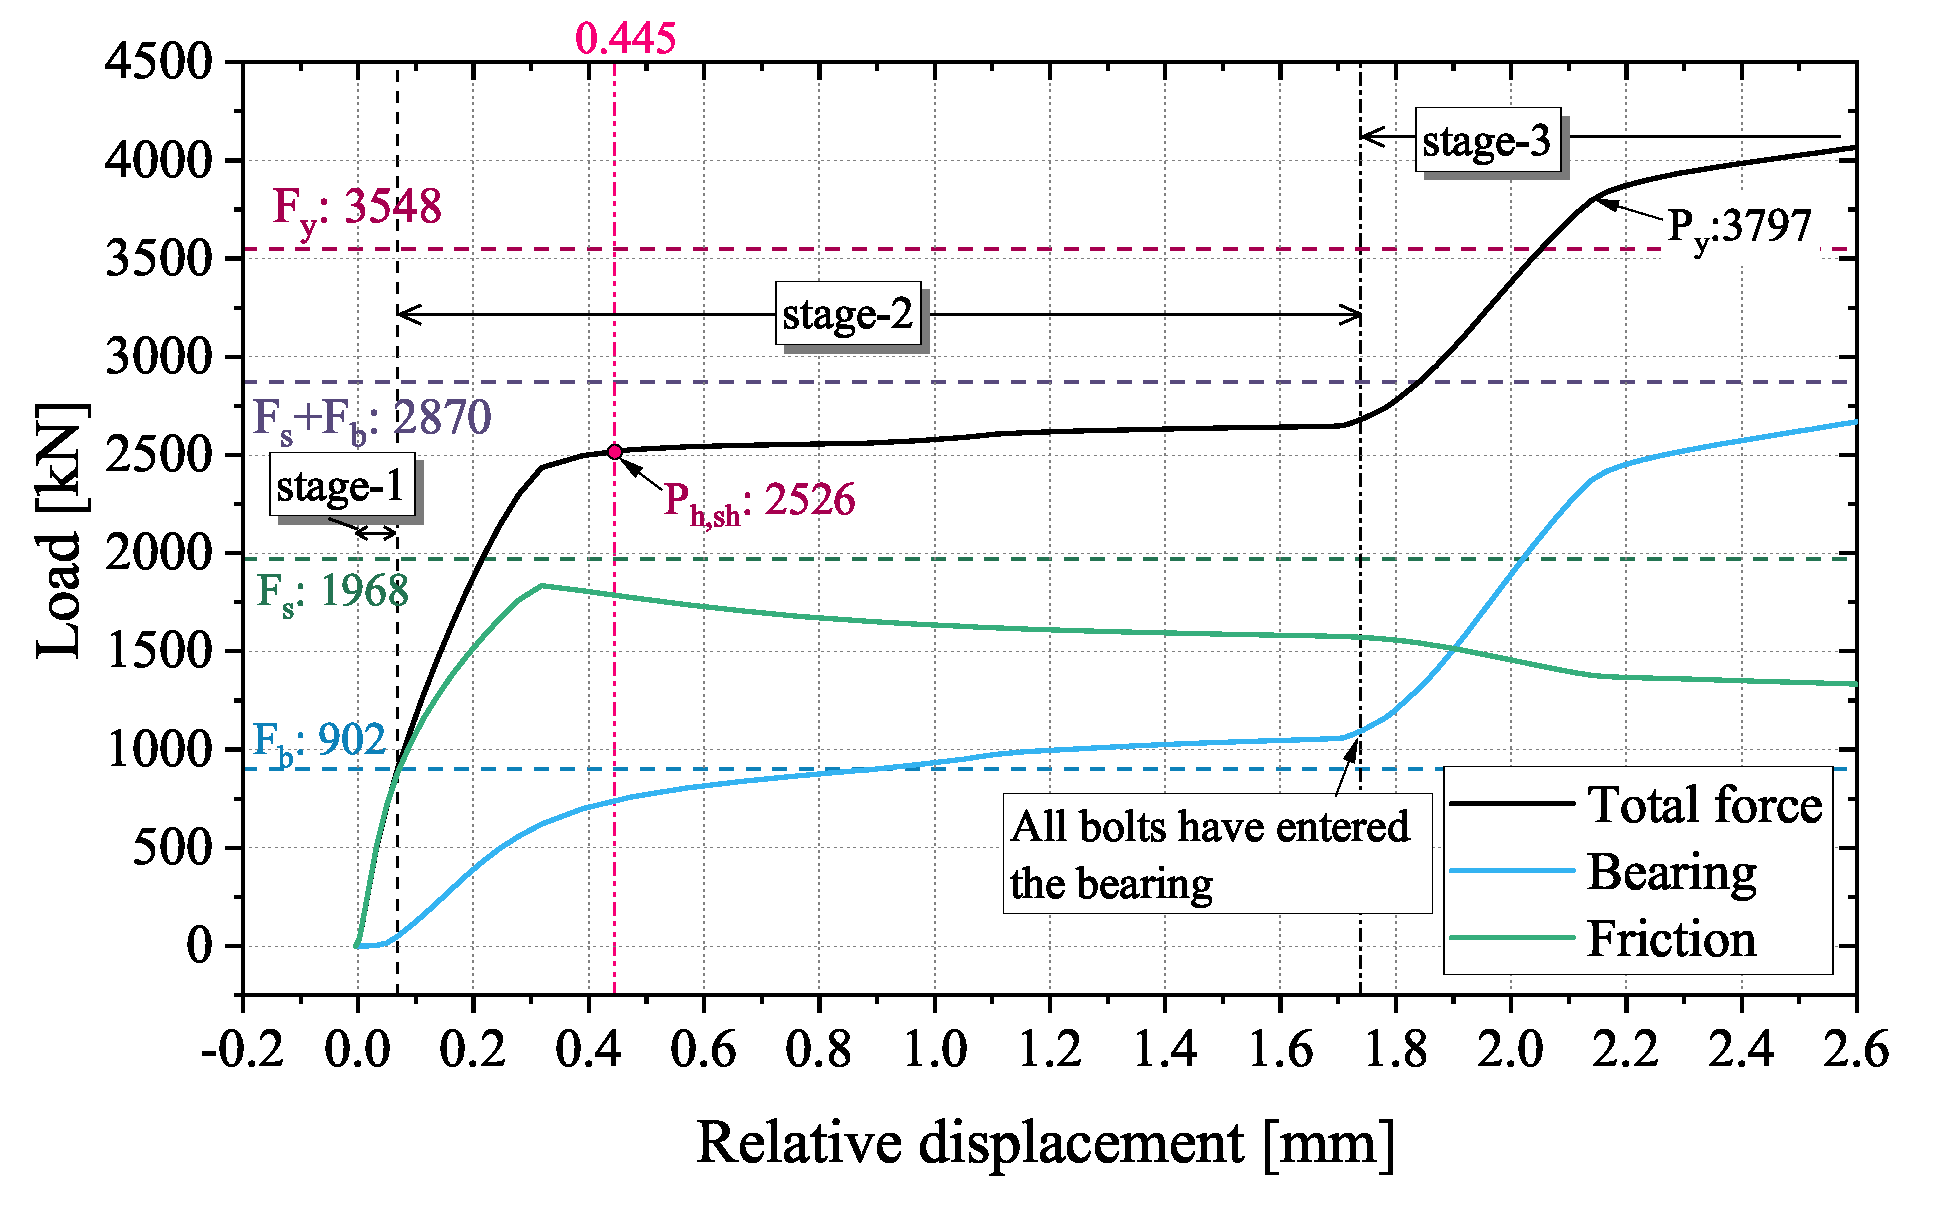
\includegraphics[width=\textwidth]{imgs/ch7/LD-OAP2B.eps}
    \caption{Bolt arrangement: 2/12 (the number of Bolt-B=4, Bolt=12), OA2B case, $\beta_h = 0.81$}
    \label{fig-ldoa2b}
\end{subfigure}
\hfill
\begin{subfigure}[b]{0.9\textwidth}
    \centering
    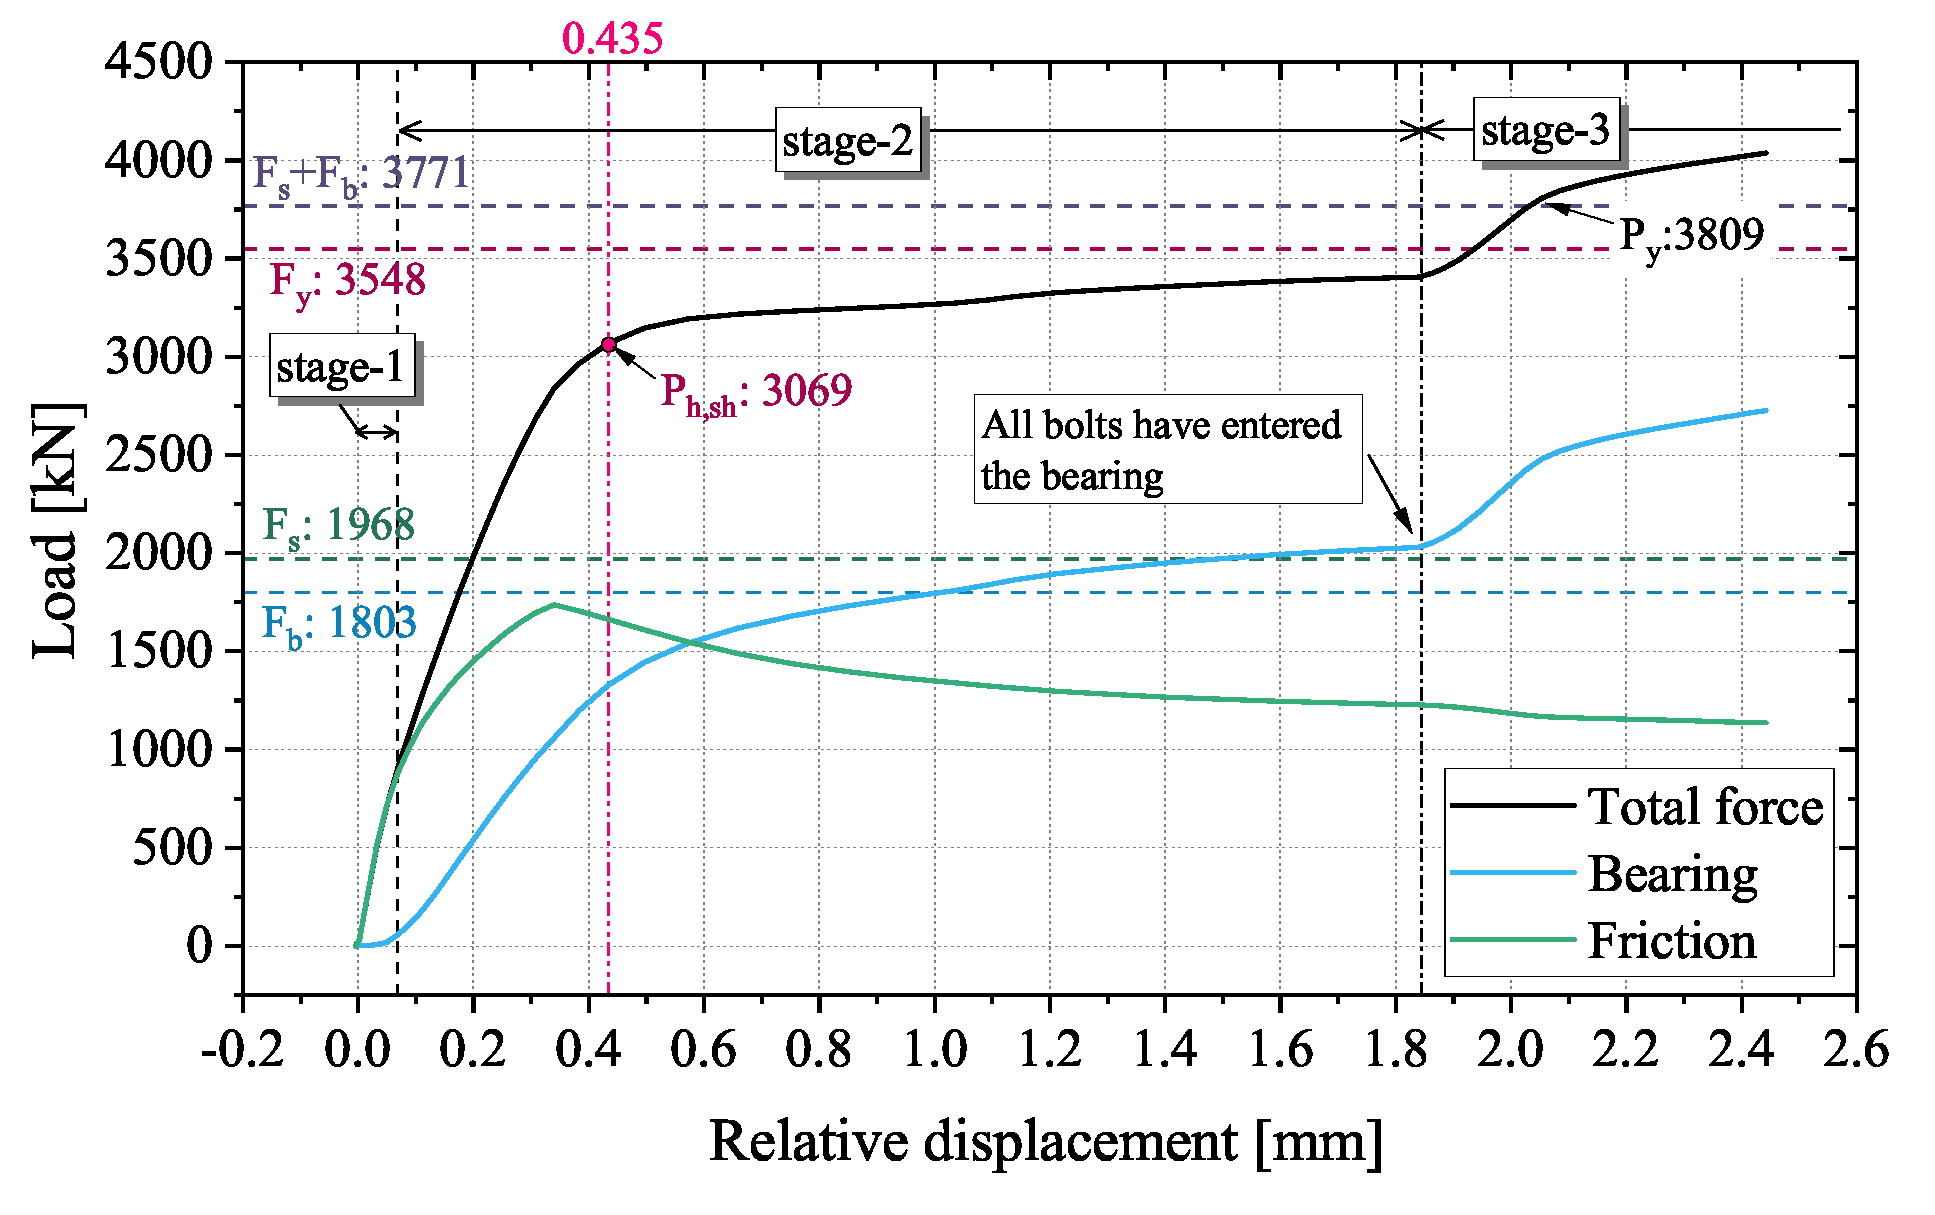
\includegraphics[width=\textwidth]{imgs/ch7/LD-OA4B.eps}
    \caption{Bolt arrangement: 4/12 (the number of Bolt-B=4, Bolt=12), OA4B case, $\beta_h = 0.81$}
    \label{fig-ldoa4b}
\end{subfigure}

\caption{Relationship between relative displacement and load (total force, bearing, friction force), SLS = Bearing}
\label{fig-loadrd-beaf}
\end{figure*}

Figure \ref{fig-loadrd-beaf} shows the relationship between relative displacement and load (total force, bearing and friction force). Relative displacement is referenced to the AIJ's \cite{AIJ2012AIJStructures} recommendation and taken from the location of a distance 10 mm from the inner end of the plate. where the green dashed line represents the frictional strength $F_s$ calculated by equation \ref{eq-fds} and the blue dashed line represents the bearing strength $F_b$ calculated by equation B. The red dashed line represents the net section yield strength $F_y$ and the cumulative value of the compressive and frictional strengths ($F_s+F_b$) is represented by the purple dashed line.

The blue solid line represents the bearing force, the green solid line represents the friction force, and the black solid line represents the total load received by the joint, as shown in Figure \ref{fig-how2cal-fbfs} the total force is taken from the integral force at the end of the main plate. The friction force is calculated by the shear stress of the faying surface in the main plate, The bearing force is the sum of the hole surface's contact pressure.

In Figure \ref{fig-loadrd-beaf}, it can be noticed that whether the case is arranged with 2 fit bolts (2/12) or with 4 fit bolts (4/12), the bearing connection hardly participates in the load transfer at the initial stage, this is due to the fact that the friction connection has a much higher stiffness than the bearing connection, and the bearing connection hardly shares the load until a certain amount of elastic slip occurs, which was also referred to by the previous study through experiments as well as analysis \cite{fisher1965behavior,chen2023mecha,chen2024Exp}. 

In this present study, the moment when load sharing starts in a bearing connection (i.e., transfer load combined with friction) is defined as stage 1. The stiffness of the joint's total force is almost determined by the stiffness of the friction connection until stage 1 is reached, after which the stiffness of the total force hardly changes although the bearing connection also starts to transmit loads, and the transition from the transmission of loads for the friction connection only to the hybrid transmission stage of friction and bearing is very gentle.

After stage 1, as the load increases, the friction connection reaches its maximum resistance, and the slope of the relative displacement curve of the joint decreases, after which the load continues to be transmitted mainly by the bearing manner. There was no significant slippage, and this was confirmed in the experiment's result \cite{chen2024Exp}, as shown in Appendix \ref{sec-valid}.

Where, in this present study, the load transfer in the bearing connection of a fit bolt starts (stage-1) until reaches the max slip resistance and all the bolts are in the bearing state, which is called the hybrid load transfer stage, i.e. stage 2.

It should be noted that in the analysis of Coulomb friction used for contact pairs, theoretically, the friction does not decrease even when the maximum value is reached, however, due to out-of-plane deformation of the splice plate, shear bending of the bolts, etc., the friction force decreases significantly, which will be explained in more detail in section \ref{sec-decoff}.

The mechanical behaviour as well as the ultimate limit state of the hybrid connection after all bolts have entered the bearing state can be approximated as a bearing-type bolted connection, which is stage-3 of the hybrid connection.

In the case of the bolt shank shear yield limit state, the hybrid joints arranged with 2 fit bolts (see Figure \ref{fig-ldoa2b}) and 4 fit bolts (see Figure \ref{fig-ldoa2b}) produce almost the same relative displacements of about 0.43 $mm$ when the bolt shank shear yield strength $P_{h,sh}$ is reached. It can be assumed that this is due to the amount of elastic deformation generated when the bolts yield in the shear plane, so if the judgement condition is the load at the shear yield strength of a bolt shank, the amount of elastic deformation generated by that bolt can be assumed to be the same. Therefore, it can be considered that when the hybrid joint reaches the bolt shank shear yield strength $P_{h,sh}$, the end position of the joint will produce a relative displacement of approximately 0.4mm (Although the elastic deformation is also related to the material of the steel, the elastic modulus of the steel in this analysis is 205 $Gpa$, so this factor is not considered.).

%在极限状态为承压的情况下,安排了4根fit螺栓和2根fit螺栓的混合接头在到达剪切屈服强度时产生的相对位移量几乎相同,均为0.4左右。可以认为这是因为螺栓发生剪切屈服时,所产生的弹性形变量,因此当判定条件固定为一根螺栓发生剪切屈服时的载荷为剪切屈服极限时,此螺栓产生的弹性形变量可以认为是相同的。因此可以认为当混合连接到达剪切屈服极限时,接头的端部位置会产生0.4mm左右的相对位移(虽然弹性变形和钢材的材质也有关,此研究钢材的弹性模量均为205Gpa,因此不考虑此因素)。

%从图中可以发现,总载荷达不到FS+Fb主要是因为摩擦力的降低,以及承压力的延迟分担,以及当任意螺栓发生轴部剪切屈服时无法到达其设计强度。%To do


Figure \ref{fig-lrd-ncy} shows the relative displacement curve of the hybrid connection when the serviceability limit state (SLS) is determined as net cross-section yielding. It can be observed that even when net cross-section yielding is taken as the SLS, the hybrid connection can still be divided into three load transfer stages. The slight difference is that due to the tensile deformation of the net cross-section, the load that can be transferred by bearing becomes less, and before reaching the net cross-section yielding, both the stiffness of friction and bearing show a noticeable decreasing trend.

%图8显示了当使用极限状态(SLS)判断为Net cross-section yield时,混合接头的相对位移曲线图。可以发现,纯断面屈服为SLS时,混合接头依然可以分为3个载荷传递阶段。稍微不同的是,由于纯断面的拉升变形,承压所能传递的载荷变得更少,在到达净界面屈服前,摩擦和承压的刚性都有明显的降低趋势。

\begin{figure*}
    \centering
    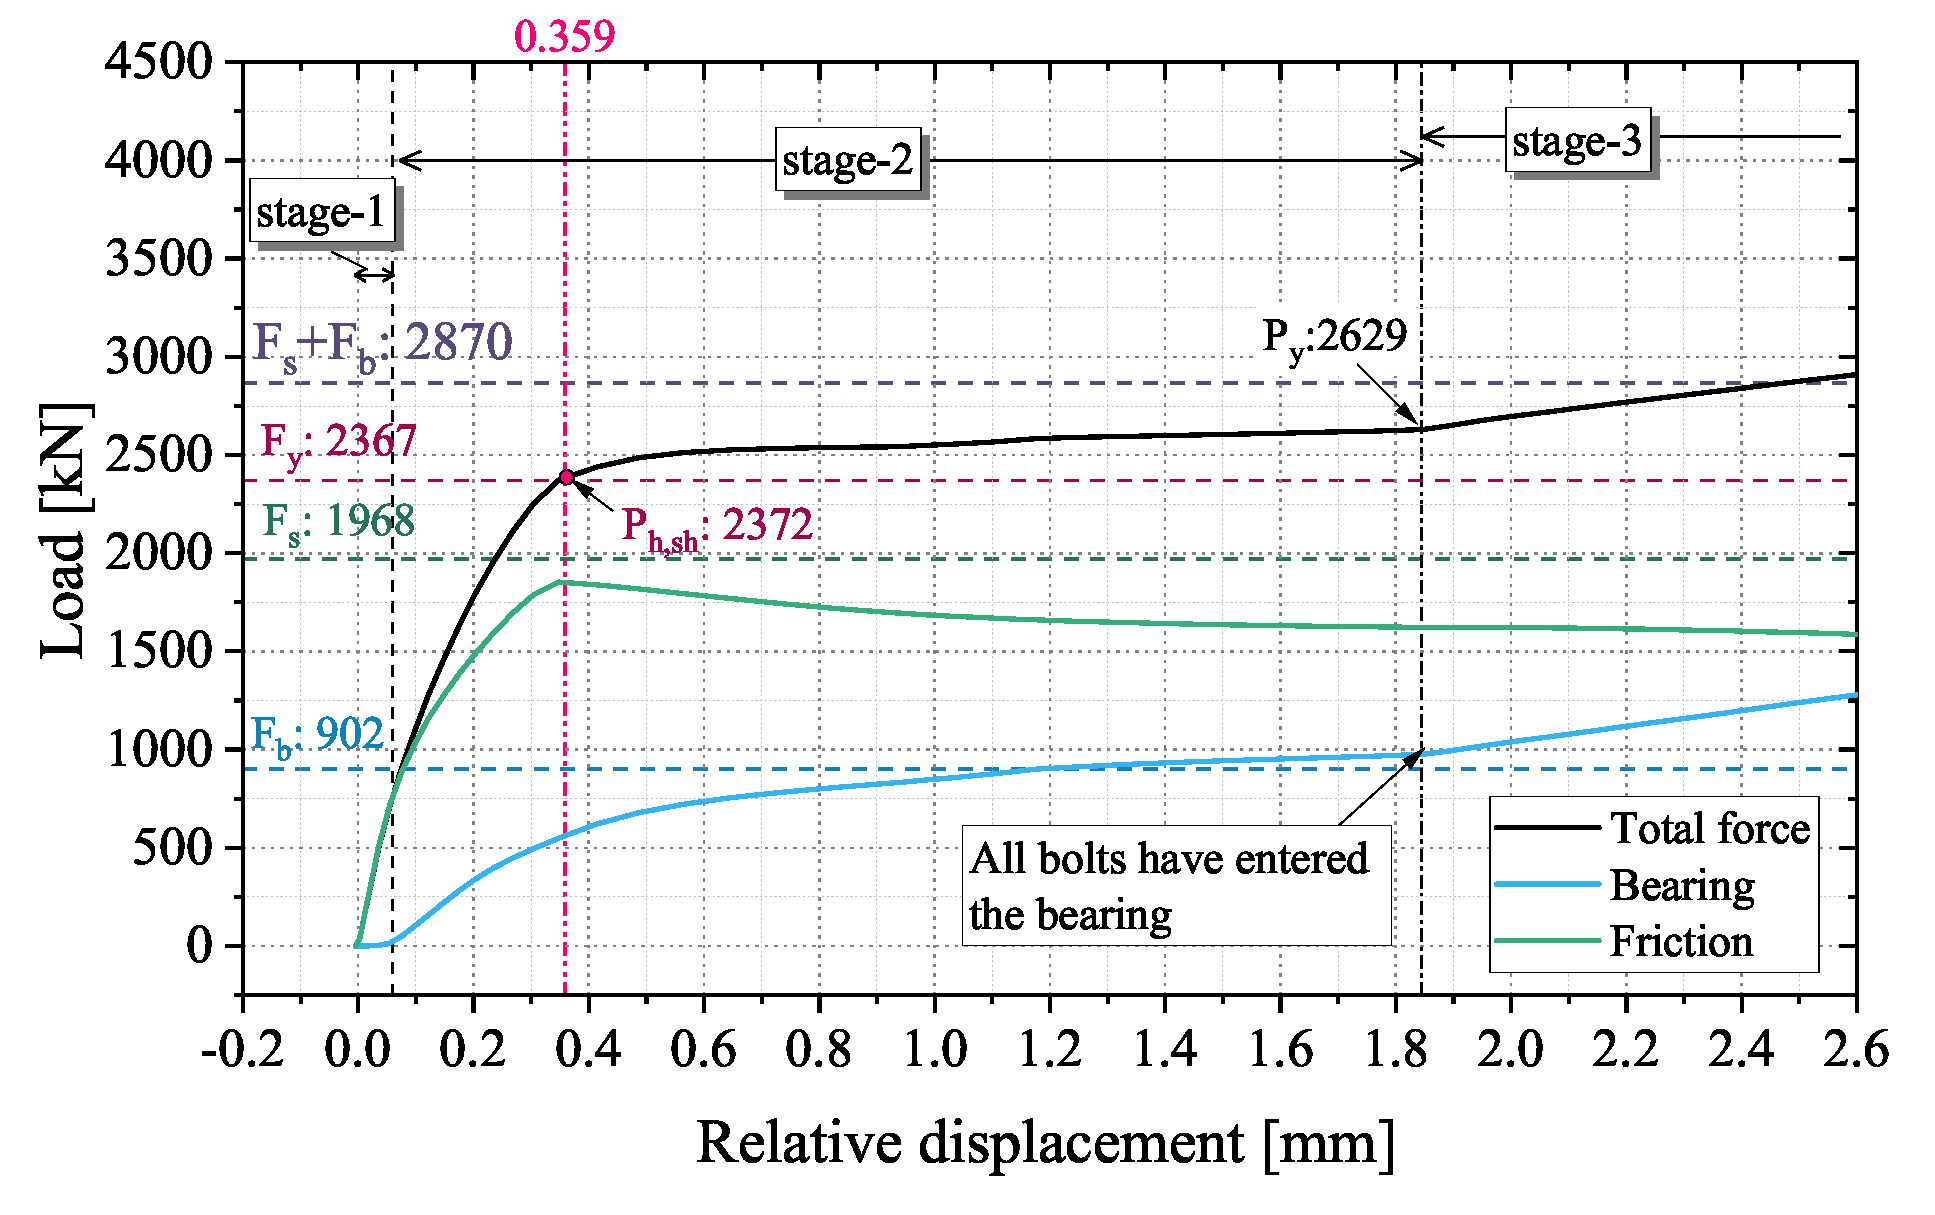
\includegraphics[width=0.9\linewidth]{imgs/ch7/LD-OAP2.eps}
    \caption{Relationship between relative displacement and load (total force, bearing, friction force), SLS = Net Cross-section yield}
    \label{fig-lrd-ncy}
\end{figure*}


\begin{figure*}
    \centering
    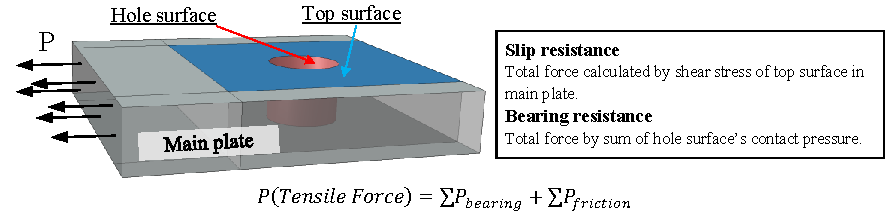
\includegraphics[width=0.9\linewidth]{imgs/ch7/how2cal-fbfs.pdf}
    \caption{Calculation methods of bearing and friction force}
    \label{fig-how2cal-fbfs}
\end{figure*}



\subsection{Relative displacement of long bolted joint}

Figure \ref{rd-distri} represents the relative displacement distribution at various locations of the hybrid long connection (taking the OA4B case as an example), where BC represents the bolt centre location, and E-10mm represents the location 10 mm away from the inner side of the joint. It can be observed that the relative displacement distribution of the connection is significantly non-uniform. When the connection reaches bolt shear yielding in the bolt shank (at SLS), the relative displacement at E-10mm is 0.43 mm. The relative displacement becomes smaller towards the middle of the connection, with only 0.12 mm at the locations of bolts \#n6 and \#n7 (BC-6, -7). The overall average relative displacement of the connection is 0.24 mm, with a median value of only 0.2 mm. The Japanese Specification for Highway Bridges (JSHB) \cite{douji2017} specifies a relative displacement of 0.2 mm when conducting slip coefficient tests on two rows of friction type connection. On the other hand, for bearing-type connections, due to their lower stiffness, there is no explicit specification for the relative displacement of the connection. This study considers the failure mode of the hybrid connection to be approximated as a bearing-type connection. Therefore, with a median relative displacement of only 0.2 mm, the relative displacement of the hybrid connection is well within an acceptable range.

%图a代表了混合长连接的接头各处的相对位移分布图(以OA4Bcase为例),其中BC代表bolt center,E-10mm代表接头距离接头内侧10mm位置。可以发现,接头的整体的相对位移分布明显不均匀,当接头在螺栓轴部剪切屈服时(SLS),端部E-10mm处的相对位移为0.43mm,约接近接头中间,接头发生的相对位移就越小,中间的6,7号螺栓处的相对位移BC-6,-7仅为0.12mm。接头的整体平均相对位移为0.24,其中位值仅为0.2mm。 日本的JSHB对使用两列摩擦连接对接头进行滑移系数测试时,规定的相对位移量为0.2mm,另一方面,对于承压型连接,由于其刚性较低,并没有对接头的滑移量做明确的规定。本研究认为的混合接头的失效方式主要近似为承压型连接,因此对于相对位移的中位数仅为0.2mm而言,混合接头的整体滑移量是完全在可接受范围内的。

\begin{figure*}
\centering
    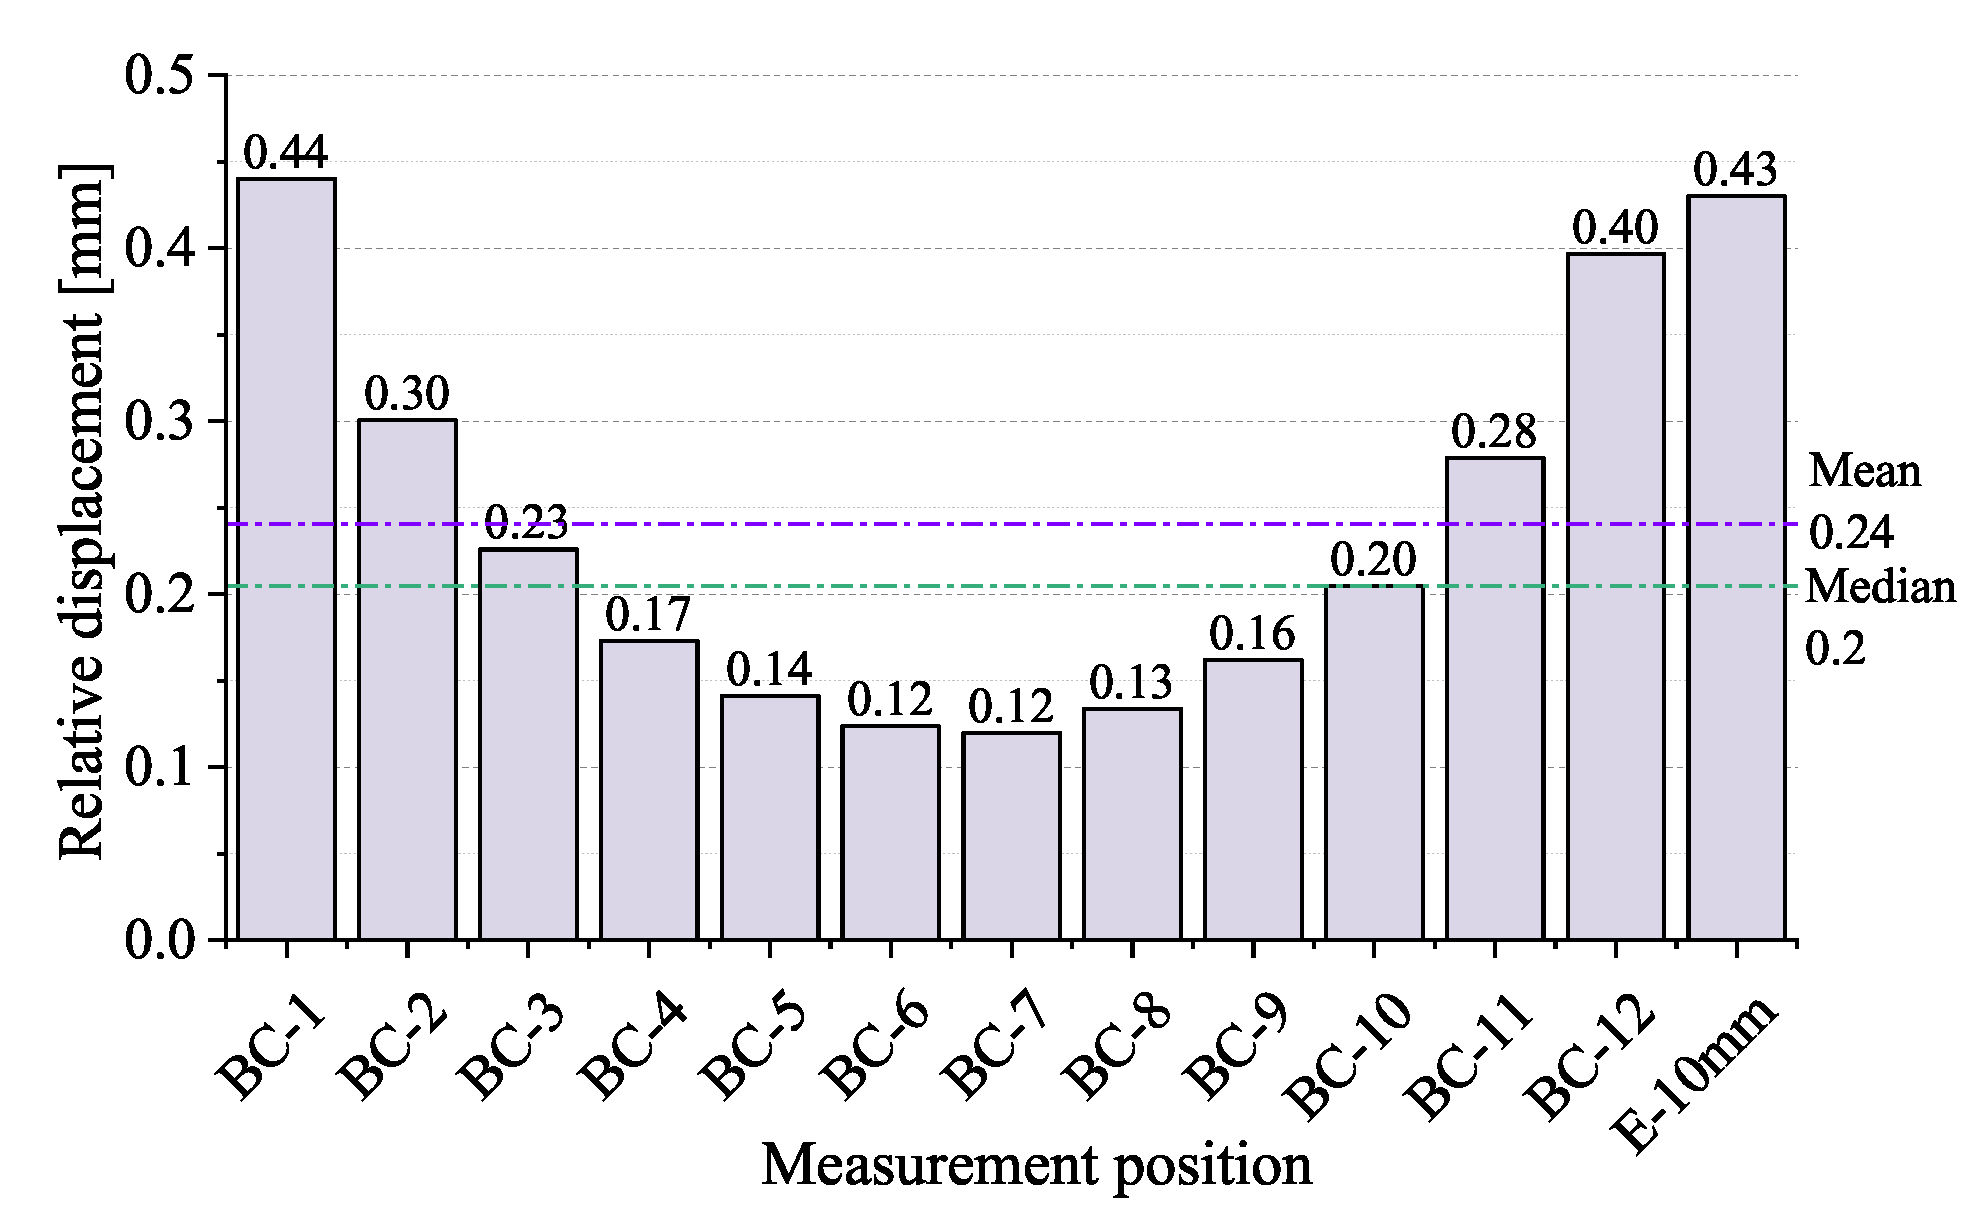
\includegraphics[width=0.9\linewidth]{imgs/ch7/RD-distri-oa4b.eps}
    \caption{Relative displacement of each measurement position in the hybrid joint (OA4B case)}
    \label{rd-distri}
\end{figure*}


\subsection{Load sharing of each bolt}
\label{LS}

%图a显示了不同的螺栓排布情况下,当载荷为螺栓轴部剪切屈服时(SLS),各个螺栓的摩擦以及承压载荷分布情况。绿色bar代表螺栓通过摩擦传递的阻力,蓝色bar代表螺栓通过承压传递的阻力。对于摩擦型长接头由于载荷分布的不均匀,在接头达到许用滑移量时,位于接头中间的螺栓无法达到其实际的设计滑移强度,因此日本的JSHB(Japanese Specification for Highway Bridges) 提出了关于摩擦型长接头的折减系数。然而,可以发现,对于混合连接无论是哪种情况,在对于中间配置的摩擦连接用螺栓有着均匀的载荷分担,且都分担了其设计滑移强度的载荷(0.4*2*205=164 kN)。另外,对于fit螺栓,由于其承压的载荷传递方式,其摩擦力有着不同程度的衰减。位于前端的#1螺栓摩擦力降低得最为严重,详细原因会在第5节解释说明。然后,对于fit螺栓分担的承压阻力,在配置的fit螺栓数量为4(也就是两端各两根)时,载荷会出现载荷分担不均的情况,虽然看起来#2螺栓分担了更多的载荷(P_b+P_s),然而前端的#1号螺栓由于衰减了几乎所有的摩擦力,因此几乎全靠承压在传递载荷,其承压阻力在所有fit螺栓中最高,因此也导致了螺栓的轴部剪切屈服也都发生在#1号螺栓,且由于承压分担的不均匀,承压阻力达不到设计的承压强度。


\begin{figure*}
    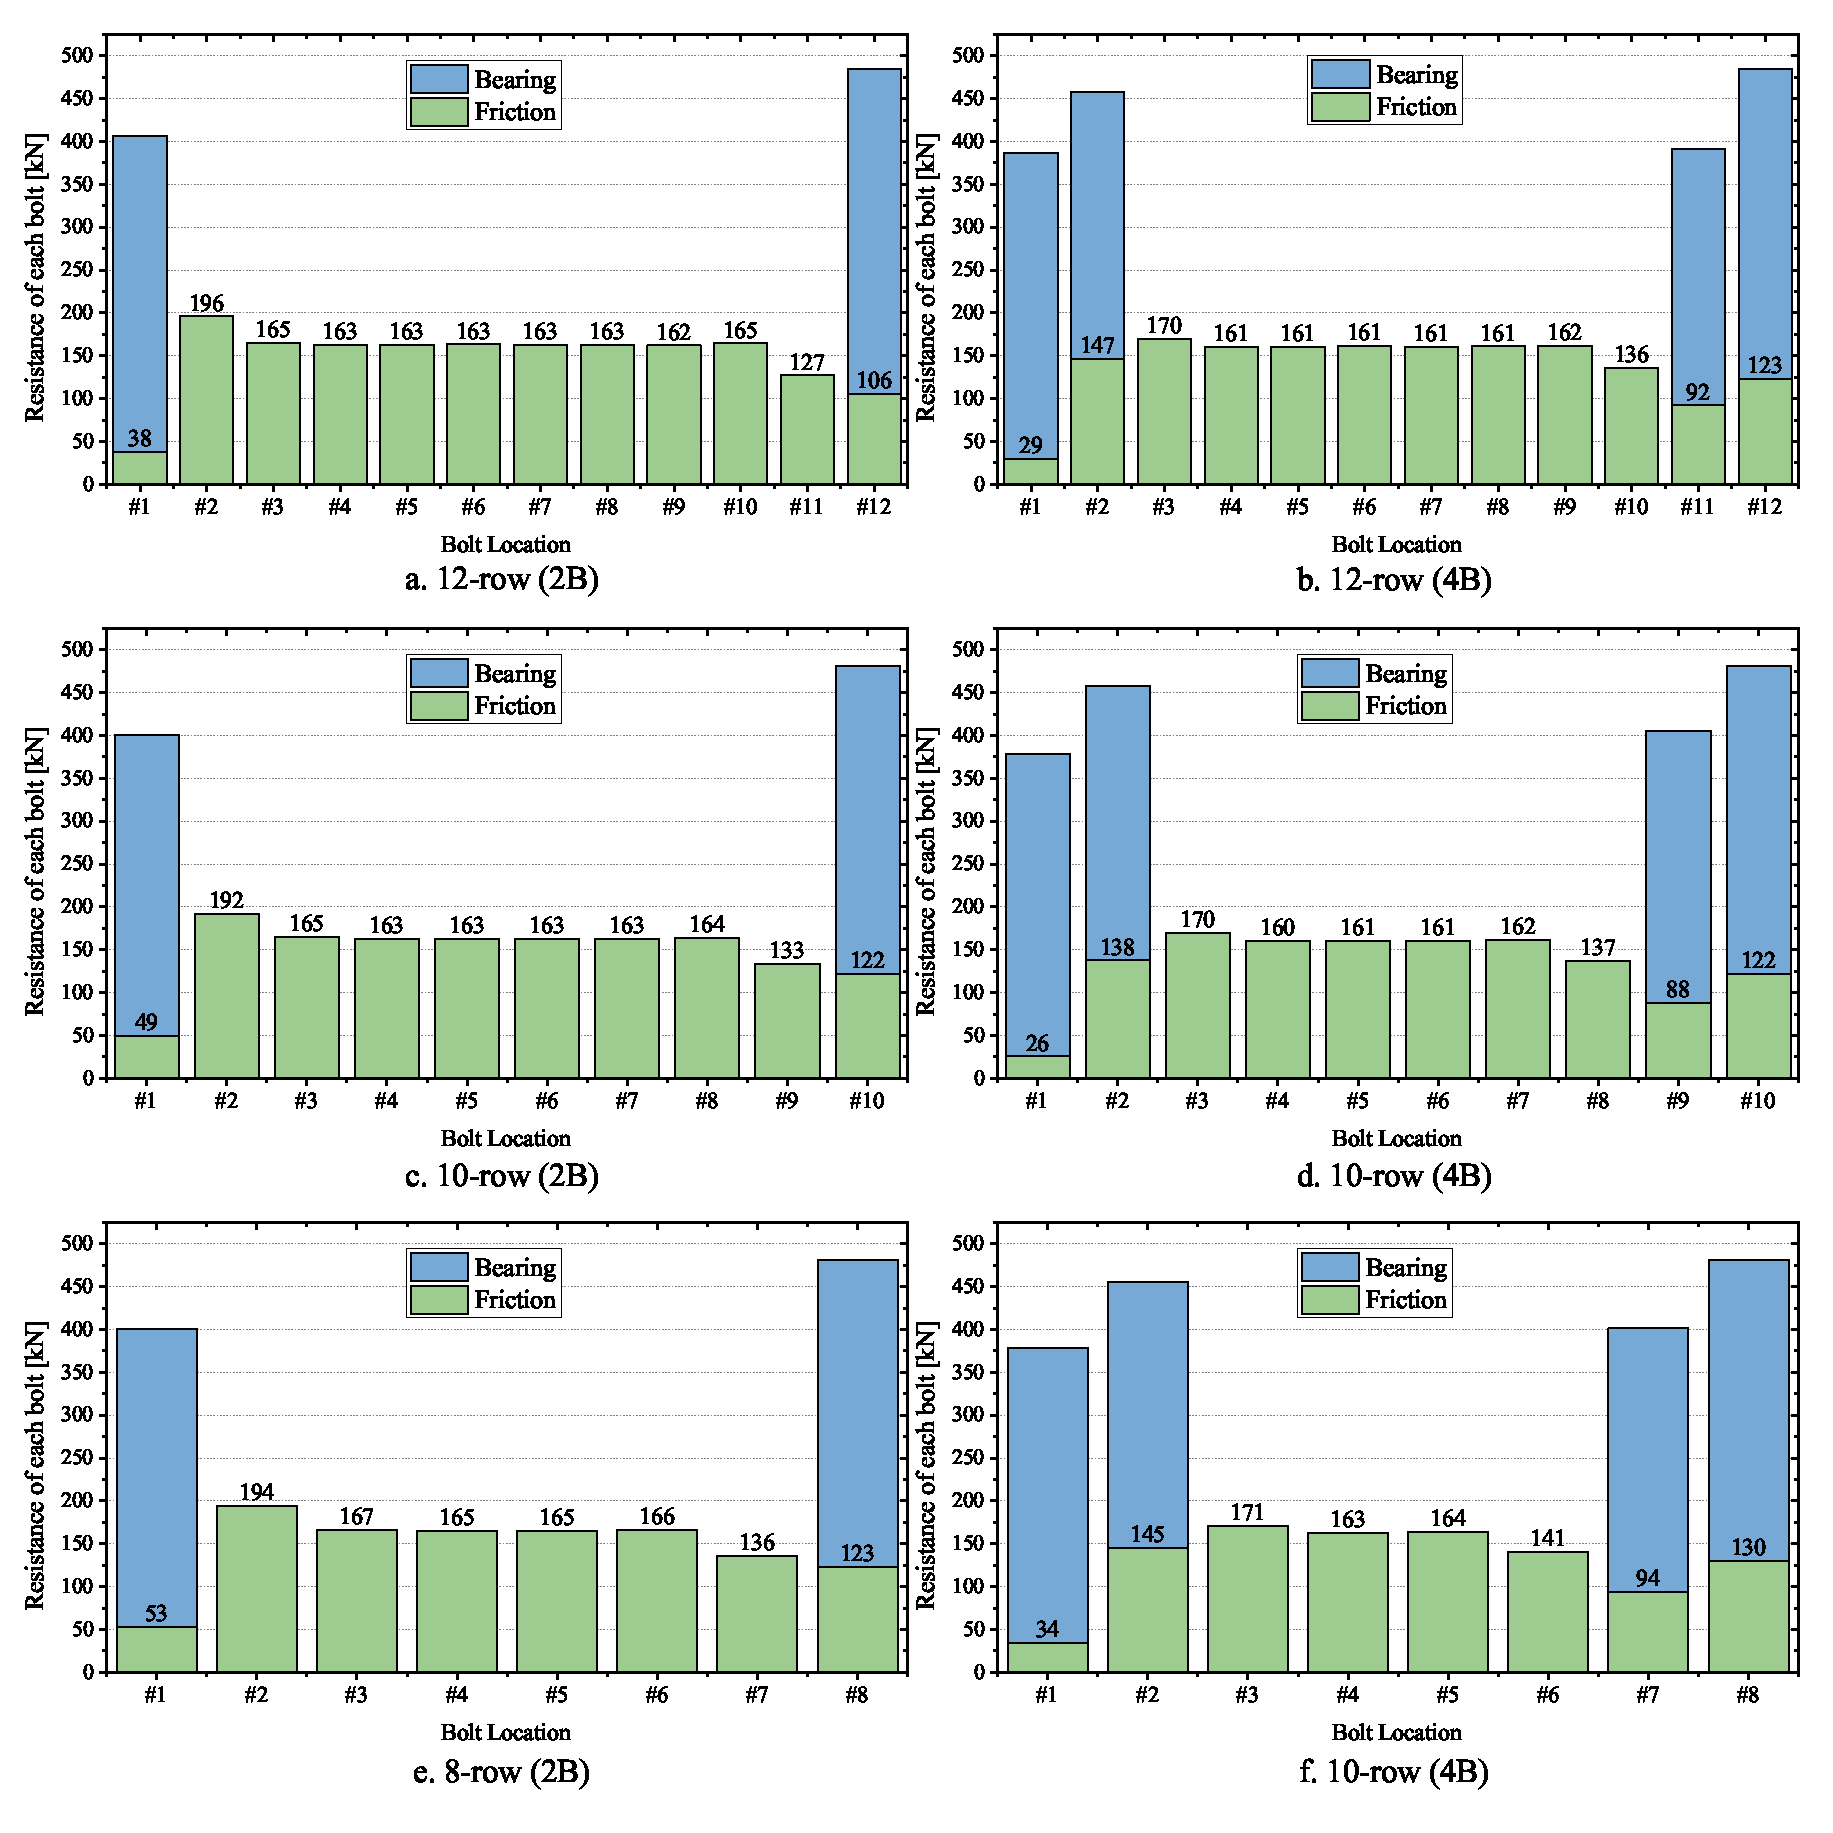
\includegraphics[width=\linewidth]{imgs/ch7/LS-all.eps}
    \caption{Load sharing of each bolt (stacked bar: $P_{s1}+P_{b1}$)}
    \label{fig-ls-all}
\end{figure*}

Figure \ref{fig-ls-all} shows the distribution of friction and bearing resistance on individual bolts when the load reaches bolt shear yielding in the bolt shank (SLS) for different bolt arrangement cases. The green bars represent the resistance transferred through friction for each bolt, while the blue bars represent the resistance transferred through the bearing. For long friction-type connections, due to the uneven load distribution, when the joint reaches the allowable slip value, the bolts located in the middle of the connection cannot reach their actual design slip strength \cite{KAMEI2000,peng2013}. Therefore, the Japanese Specification for Highway Bridges (JSHB) \cite{douji2017} proposed a reduction factor for long friction-type connections. However, it can be observed that for hybrid connections, regardless of the case, the bolts for friction type connection arranged in the middle have a uniform load sharing, and all bear the load of their design slip resistance ($F_s = \mu m N=0.4\times2\times205 = 164 kN$). Additionally, for the fit bolts, due to their bearing load transfer mechanism, their friction force experiences varying degrees of reduction. The \# 1 bolt at the front experiences the most severe reduction in friction resistance, and the detailed reason will be explained in Section \ref{sec-decoff}. Then, for the bearing resistance borne by the fitted bolts, when the number of fitted bolts is 4 (i.e., two at each end), an uneven load sharing occurs. Although it appears that \# 2 bolt bears more load ($P_b + P_s$), the \# 1 bolt at the front has almost no friction force left due to the deformation, and thus it relies almost entirely on bearing to transfer the load. As a result, its transferred bearing resistance is the highest of all the fitted bolts, causing the shank shear yield to occur first in the \# 1 bolt. In addition, the bearing resistance $P_{b}$ does not reach the design bearing strength $F_b$ due to the uneven bearing load distribution.




\subsection{Reduction of friction force}
\label{sec-decoff}

\begin{figure*}
    \centering
    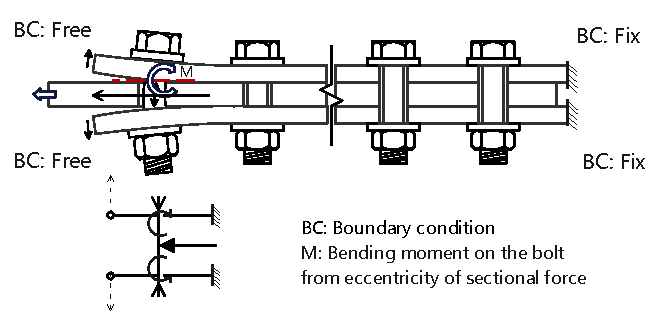
\includegraphics[width=0.85\linewidth]{imgs/ch7/OP-def.pdf}
    \caption{Schematic diagram of out plane deformation for splice plates}
    \label{fig-OP-def}
\end{figure*}

The cross-sectional force acting on the main plate is divided into the cross-sectional forces of the main plate and splice plates via the shear transmit on the bolt as shown in Figure \ref{fig-OP-def}. Assuming that the point of action of each cross-sectional force is at the centre of the plate, an additional bending moment is generated in the bolt due to the eccentricity of the cross-sectional forces. The boundary condition at the end of the connection plate is free, so there is a tendency to deform outward toward the main plate faying surface when subjected to additional bending moments, resulting in a separation of the connection plate from the main plate, and therefore a loss of contact pressure.



\begin{figure*}
    \centering
    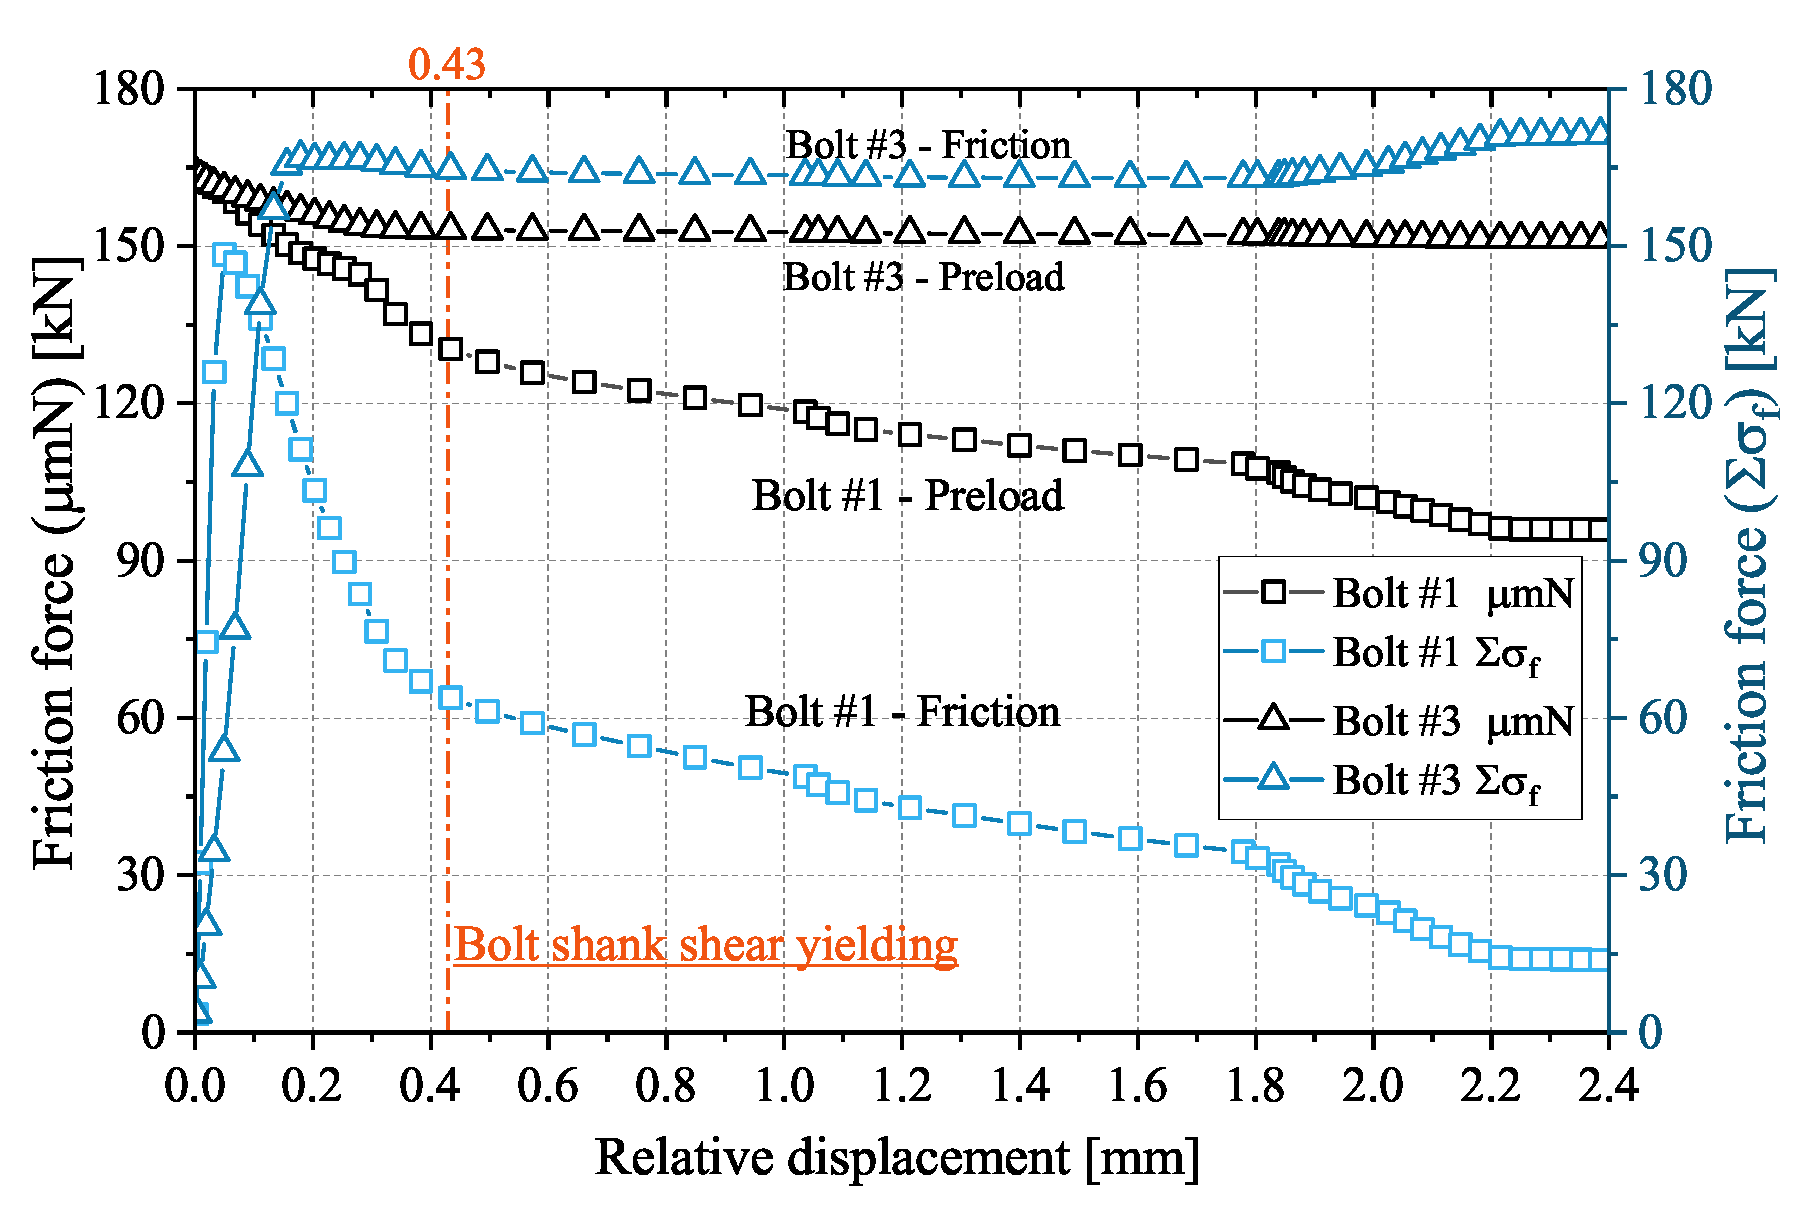
\includegraphics[width=0.7\linewidth]{imgs/ch7/RD2NF.eps}
    \caption{Relationship between \#1 bolt's friction force, \#1 bolt's preload ($N/N_0$) to relative displacement (OA4B case).}
    \label{fig-RD2NF}
\end{figure*}

Figure \ref{fig-RD2NF} showed the Relationship between friction force, bolt preload ($N/N_0$) to relative displacement. The blue color represents the friction force taken from one bolt, and the black color represents the preload of the bolt, which is obtained through the built-in bolt load option in Abaqus. It can be observed that due to the shear deformation of bolt \#1, it experiences a loss of preload, causing the friction force to exhibit a similar decreasing trend. However, the Bolt-F located at position \# 3 does not undergo shear bending, so its preload and the resulting friction force do not change significantly.
%蓝色代表了摩擦力,黑色代表螺栓的轴力,轴力通过abaqus自带的bolt load option获得。可以发现,由于由于\# 1号螺栓受剪变形导致了轴力的丢失,从而使得摩擦力也有着同样的趋势的下降。而位于位置\# 3的bolt-F没有发生受剪弯曲,因此螺栓的轴力以及其产生的摩擦力没有发生太大的改变。


\begin{figure*}
    \centering
    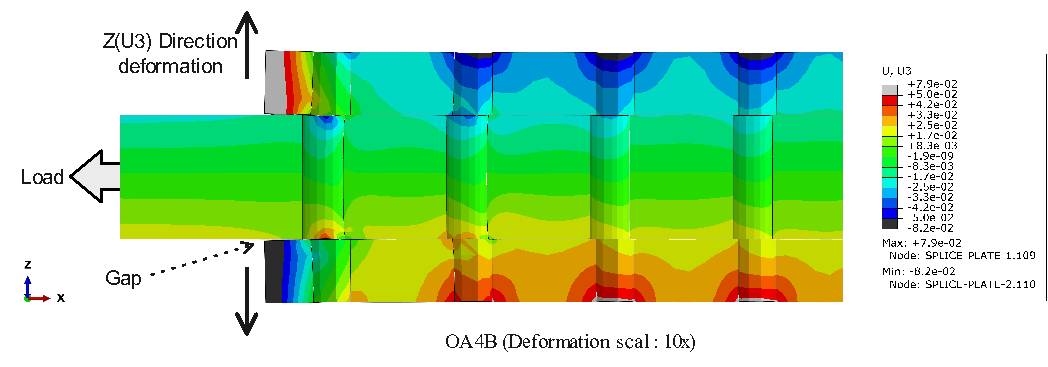
\includegraphics[width=0.85\linewidth]{imgs/ch7/OP-def-ana.pdf}
    \caption{The counter of U3 (z) direction deformation when the bolt shank shear yield occurs (Relative displacement E-10mm = 43). (Deformation scale: 10X).}
    \label{fig-OP-def-ana}
\end{figure*}


\begin{figure*}
    \centering
    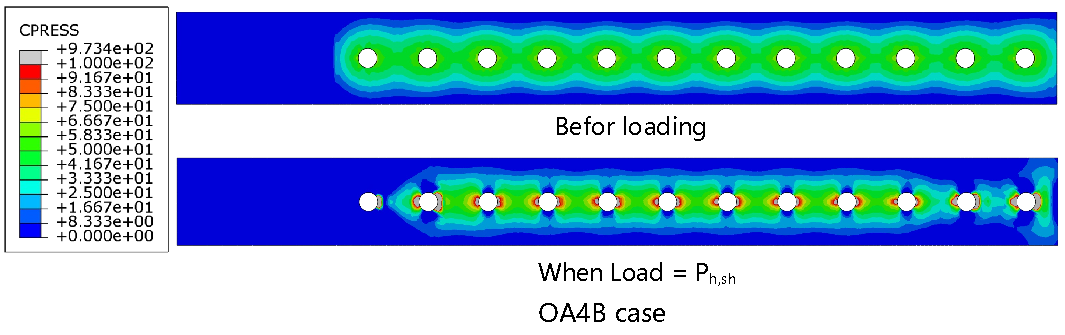
\includegraphics[width=0.8\linewidth]{imgs/ch7/OA4B-cpress.pdf}
    \caption{C-Press contour view of faying surface}
    \label{fig-cpress}
\end{figure*}

Figure \ref{fig-OP-def-ana}. shows the deformation contour plot of the joint in the U3 (z) direction, where it is evident that the splice plate undergoes deformation due to the additional bending moment generated. When the connection is at bolt shank shear yielding (SLS), the relative displacement at E-10mm is 0.43 mm, while the maximum out-of-plane deformation U3 (in the z-direction) at the end is 0.07 mm.
In the compressed side of the bolt where the bolt generates additional bending moment, due to bolt deformation, higher contact pressure is generated at the compressed side, as observed in Figure \ref{fig-cpress}. However, there is an overall decreasing trend in the total contact pressure of the faying surface.



\subsection{Reduction of bearing force} \label{sec-rduc-bea}


\begin{figure*}
    \centering
    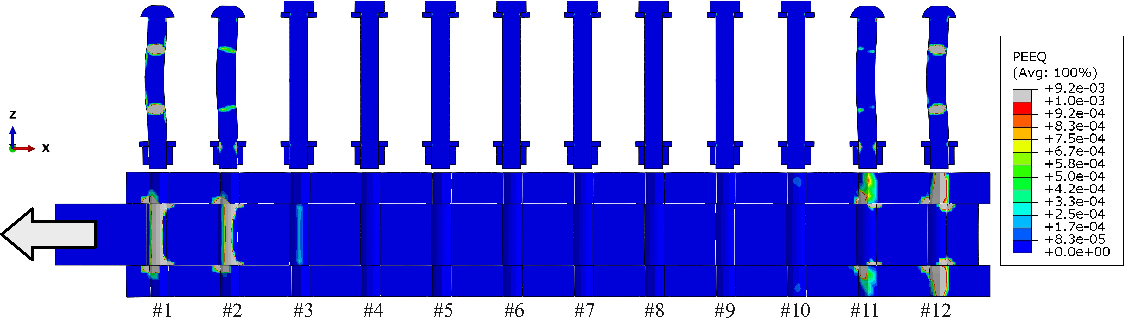
\includegraphics[width=0.9\linewidth]{imgs/ch7/beadist.pdf}
    \caption{The counter of PEEQ when the bolt shank shear yield occurs (OA4B case)}
    \label{fig-bsh}
\end{figure*}


%图15显示了当OA4Bcase中#1号螺栓发生轴部剪切屈服时,螺栓和钢板的PEEQ云图。可以发现,端部各布置两根螺栓时螺栓受到的承压力分布非常不均匀,当\#1螺栓发生剪切面屈服时,\#2螺栓的剪切面刚开始进入塑性延展。由于对称性,\#11 和 \#12号螺栓有着几乎相同的表现。这和在第2节总结的螺栓分担里的分析一致。
Figure \ref{fig-bsh} shows the PEEQ (Equivalent Plastic Strain) contour for the bolt and steel plate when bolt \#1 experiences shank shear yielding $P_{sh,h}$ in the OA4B case. It can be observed that when two bolts are arranged at each end, the bearing forces on the bolts are distributed extremely unevenly. When bolt \# 1 experiences yielding at the shear plane, the shear plane of bolt \# 2 has just entered plastic elongation. Due to symmetry, bolts \# 11 and \# 12 exhibit almost the same behaviour. This is consistent with the investigation of bolt load sharing summarized in Section \ref{LS}.



\subsection{Reduction factor for hybrid connection}

%图中显示了分别将将$P_{sh,h}$和$F_{b,h}$对$F_y$进行归一化之后的关系图。可以发现,无论螺栓如何配置(接头长度,螺栓间距等)改变,当fit螺栓(用于承压的螺栓,bolt-B)为两根时(两端各一根),$P_{sh,h}$相对于$F_{b,h}$的降低率收敛在0.867(Slope factor)左右,可以通过式1来表示.



\begin{figure*}
    \centering
    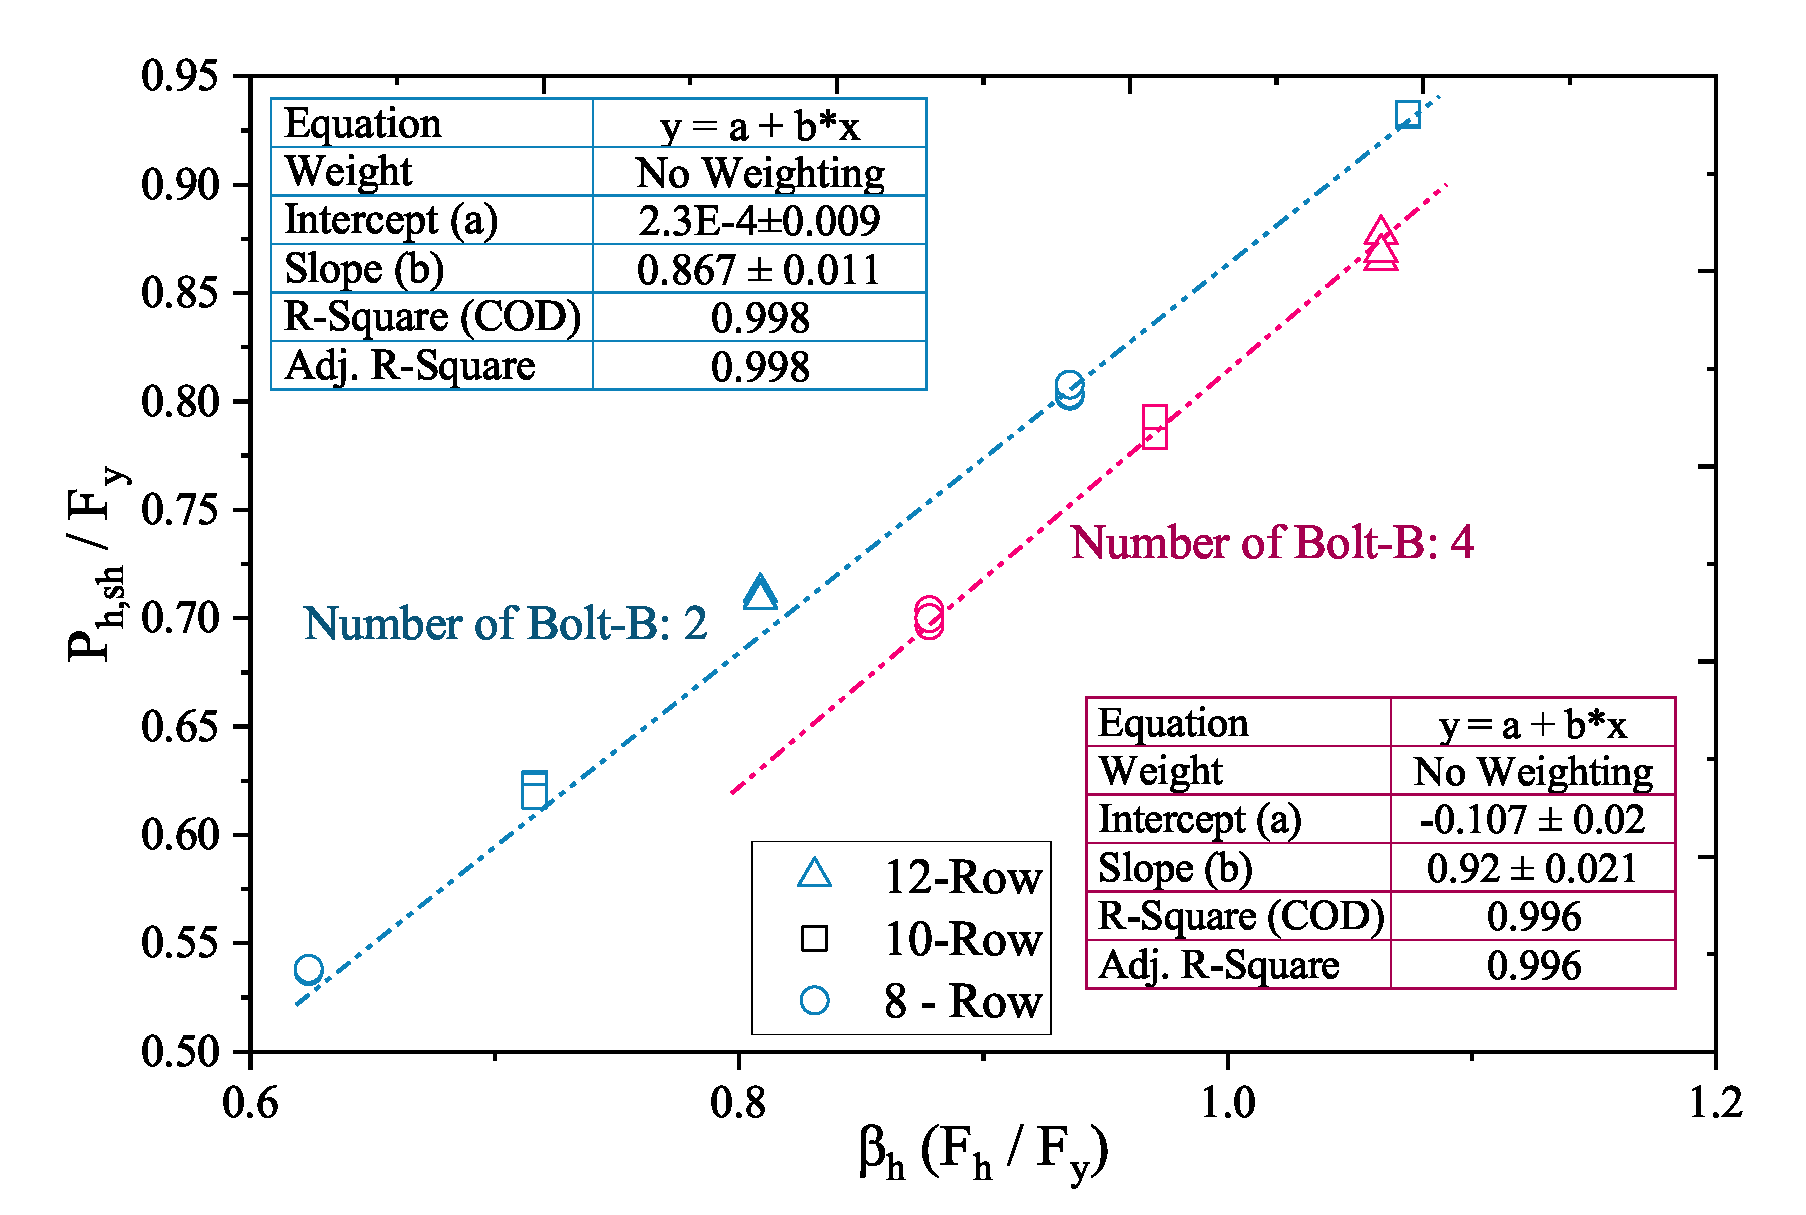
\includegraphics[width=0.85\linewidth]{imgs/ch7/pser-py.eps}
    \caption{Relationship between the nominated load $P_{h,sh} / F_y$ and the ratio}
    \label{fig-pser-py}
\end{figure*}


Figure \ref{fig-pser-py} shows the relationships after normalizing $P_{sh,h}$ and $F_{b,h}$ with respect to $F_y$. It can be observed that regardless of the bolt arrangement (joint length, bolt spacing, etc.) is changed, when there are two fitted bolts (bolts for bearing, bolt-B), the decrease rate of $P_{sh,h}$ relative to $F_{b,h}$ converges around 0.867 (Slope factor in figure), which can be expressed by Equation \ref{eq-rd-2}.

\begin{equation}
\begin{aligned}
    P_{h,sh}/F_{y} &= 2.3\times10^{-4} + 0.867 F_{b,h} / F_y \\
        F_{h,sh} &= 2.3\times10^{-4} F_y + 0.867 sF_{b,h}
\end{aligned}
 \label{eq-rd-2}
\end{equation}

%这里省略掉2.3E-4,从而进一步折减F_{b,h},式子可以表示为(当$n_b$为2时):
Here, $2.3\times10^{-4} F_y$ term is omitted, further reducing $F_{h,sh}$, and the equation can be expressed as (when $n_b$ is 2):
\begin{equation}
    F_{h,sh,cor} = 0.85 F_{h,sh}
    \label{eq-fbh2-1}
\end{equation}

%而fit螺栓为4根时,降低率大约为0.92, 然而由于承压的分担不均匀,需要另外进行折减,这里通过近似公式给出了 $-0.1F_y$的额外折减系数,
When there are 4 fitted bolts, the decrease rate is approximately 0.92. However, due to the uneven distribution of bearing forces, an additional reduction is needed. Here, an approximate formula provides an extra reduction factor of $-0.1F_y$ as shown in Equation \ref{eq-fbh4-1}.

\begin{equation}
    \begin{aligned}
      P_{sh,h}/F_{y} & = -0.107 + 0.92 F_{h,sh} / F_y \\
      F_{sh,h,cor-1} &=  0.92 F_{h,sh} - 0.1 F_y
      \label{eq-fbh4-1}
    \end{aligned}
\end{equation}



\begin{figure}
    \centering
    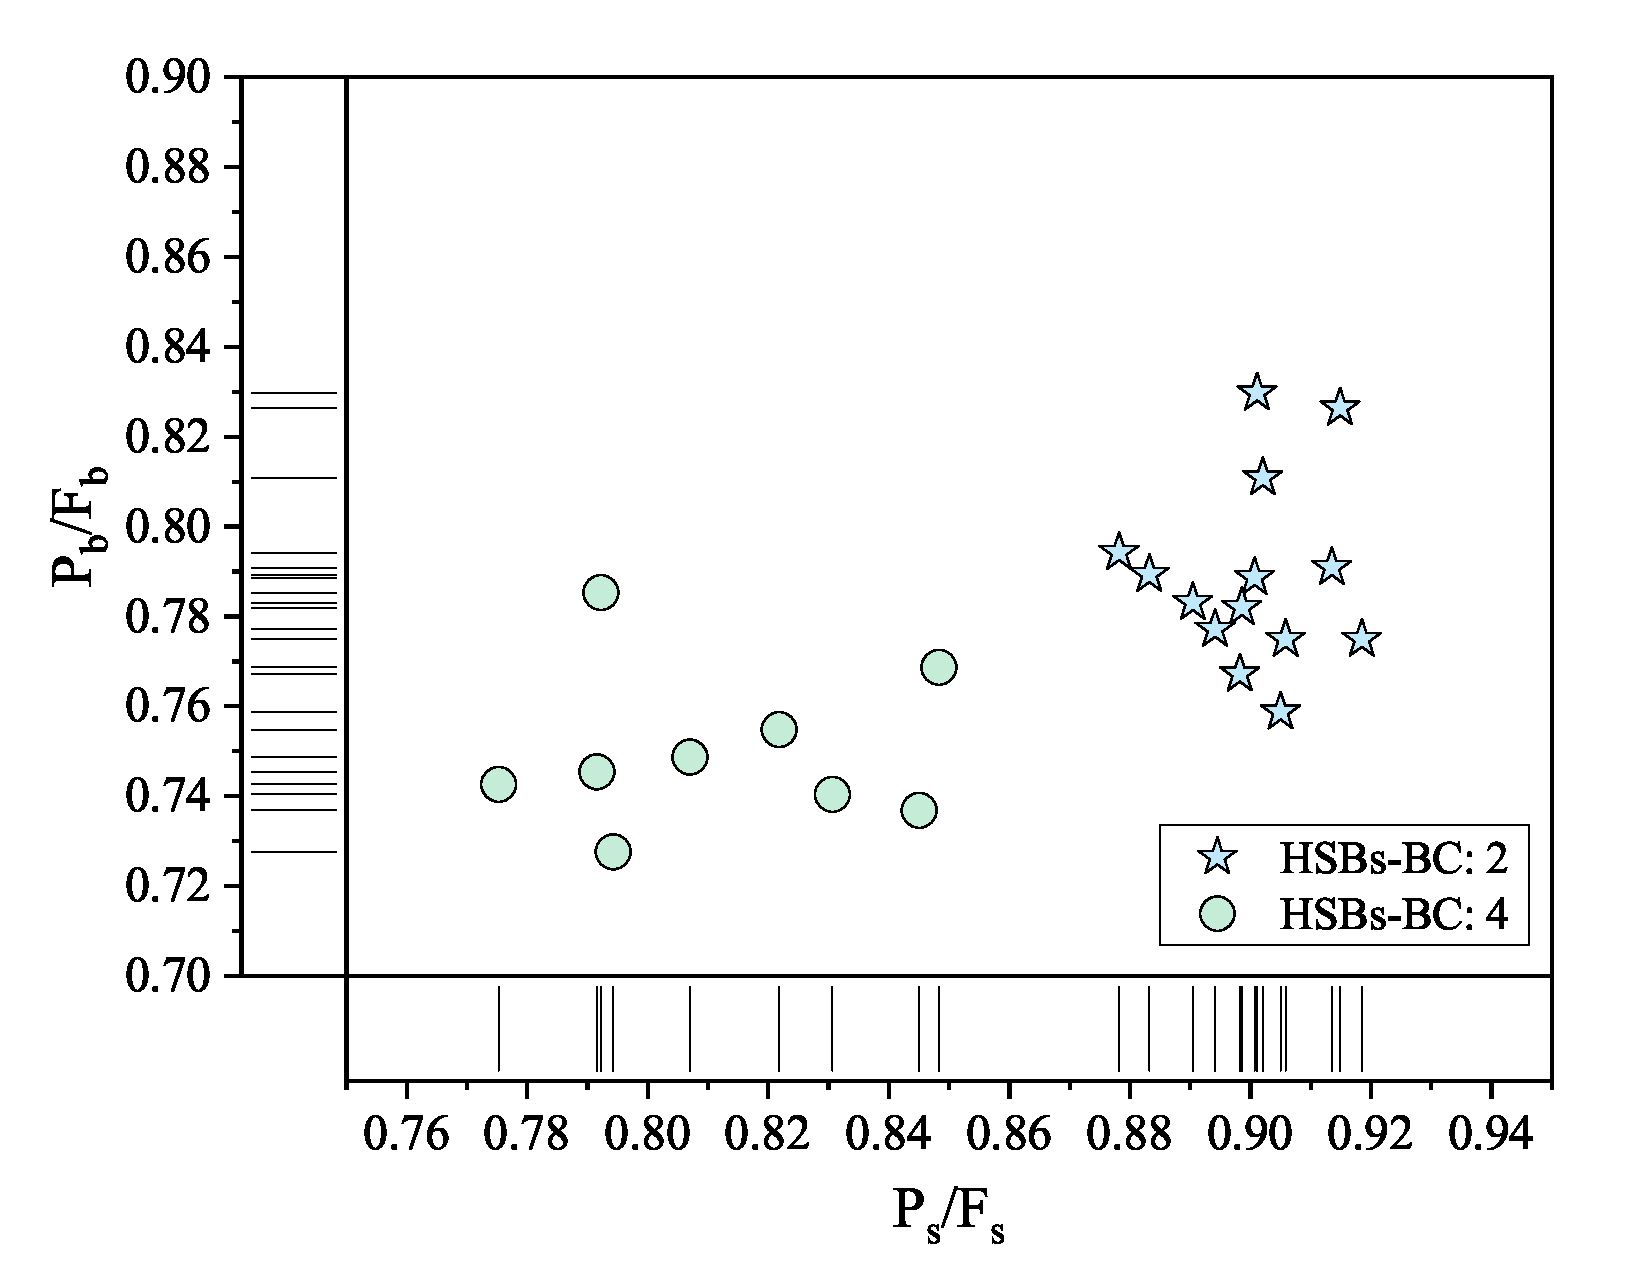
\includegraphics[width=0.85\linewidth]{imgs/ch7/RF-pspb.eps}
    \caption{Distribution of reduction rates of bearing/friction resistance}
    \label{fig-dist-RF}
\end{figure}

Due to the different load transfer mechanisms of friction and bearing, this paper also explored the reduction of friction force and bearing force separately to more accurately evaluate the bolt shank shear yielding strength of the hybrid connection. Calculation formulas for the reduction factors based on the friction force and bearing force, respectively, are proposed, as shown in Equation \ref{eq-pvh-2}. Figure \ref{fig-dist-RF} plots the reduction rates of friction force ($P_s/F_s$) and bearing force ($P_b/F_b$) for each case. It can be observed that the distribution range of the friction force reduction rate ($P_s/F_s$) is larger than that of bearing ($P_b/F_b$). For the reduction rates of friction force, the cases with 4 fitted bolts (green circles in the figure) are widely scattered, while the cases with 2 fitted bolts (blue pentagons in the figure) are concentrated within a smaller range ($0.9 \pm 0.02$). This is because when there are only 2 fitted bolts, apart from the friction force of bolt \# 1 being ignored, the friction force reduction of the fitted bolt at the other end does not vary significantly between each case. However, for the cases with 4 fitted bolts, due to the uneven distribution of bearing loads, their friction forces are also affected to varying degrees. Therefore, when there are 4 fitted bolts, the variation in the friction force reduction rate is slightly larger. For the bearing force, the variation of the reduction rate is relatively small, the reduction rates of the cases with 4 fitted bolts are concentrated around 0.74, while the cases with 2 bolts are concentrated around 0.79.
%由于摩擦力和承压力的降低机理不同,本文也分别对摩擦力和承压力的折减进行了探讨以更精确的评价混合连接螺栓轴部剪切屈服强度。图17 plot了各个case关于摩擦力的降低率($P_s/F_s$)和承压力的降低率($ P_b/F_b$). 可以发现摩擦力的降低率($P_s/F_s$)的分布范围要大于($P_b/F_b$)。对于摩擦力的降低,配置了4根fit螺栓的case(见图中绿色圆圈)散布范围很广,而配置了两根fit螺栓的case(图中蓝色五角星)集中在一个较小的范围内($0.9±0.02$),这是因为当fit螺栓数量仅为2时,除了\#1螺栓的摩擦力不考虑之外,另一侧端部的fit螺栓的摩擦力降低不会发生太大的变动,而对于fit螺栓4根的情况,由于受到的承压载荷分担不均,其摩擦力也会受到不同程度的影响,因此,fit螺栓为4根时,摩擦力降低率的变动略大。对于承压力,配置了4根fit螺栓的case降低率集中在0.74附近,而配置了2根螺栓的case集中在0.79附近。



\begin{table*}[]
    \centering
    \caption{Reduction factor of bearing and friction force}
    \scalebox{0.8}{
    \begin{tabular}{@{}cccccccccc@{}}
    \toprule
     & N total & Mean & SD & SE & Lower 99\% CI &Upper 99\% CI & Minimum & Median & Maximum \\ \midrule
     $P_b/F_b$ & 26 & 0.774 & 0.027 & 0.006 & 0.76 & 0.79 & 0.728 & 0.775 & 0.83 \\
     Bolt-B: 2 & 14 & 0.79 & 0.021 & 0.006 & 0.775 & 0.803 & 0.759 & 0.786 & 0.83 \\
     Bolt-B: 4 & 9  & 0.75 & 0.018 & 0.006 & 0.735 & 0.765 & 0.728 & 0.745 & 0.785 \\ \midrule
     $P_s/F_s$ & 26 &0.866 & 0.048 &0.01 &0.84 &0.89 &0.775 &0.89 &0.919 \\
     Bolt-B: 2 & 14 & 0.9 & 0.011 & 0.003 & 0.892 & 0.908 & 0.878 & 0.901 & 0.919 \\
     Bolt-B: 4 & 9  & 0.812 & 0.026 & 0.009 & 0.79 & 0.834 & 0.775 & 0.807 & 0.848 \\
     \bottomrule 
    \end{tabular}}
    \label{tab-rdfactor}
\end{table*}

Table \ref{tab-rdfactor} summarizes the load reduction rates of the bearing force and friction force for the cases with two fitted bolts and four fitted bolts, respectively, and provides simple statistical distributions. It can be observed that for the bearing force load reduction rate, regardless of the overall reduction rate or the cases with two or four bolts, the standard error (SE) is very small at 0.006. However, for the friction force reduction rate, the case with two fitted bolts has an SE of 0.003, while the case with four fitted bolts has an SE of 0.009, indicating a larger deviation range. Additionally, it can be seen that for both cases, the upper-lower range of the 99\% confidence interval (CI) for the bearing force reduction rate is within 0.03, suggesting that the deviation of the bearing force reduction rate is small and the data is relatively accurate. Therefore, this study adopts the lower 99\% CI value (0.76) of all bearing force data as the reduction factor $\alpha_v$ for the bearing force. On the other hand, since the distribution range of the friction force reduction rate is relatively larger than that of the bearing force, and the impact on the reduction rate differs between the cases with two fit bolts and four fit bolts, the lower 99\% CI values for the cases with two bolts and four bolts are taken separately as the reduction factor $\alpha_s$ for the friction force, as shown in Equation \ref{eq-as}.
%表1分别总结了配置两根fit螺栓和4根螺栓时,承压力和摩擦力的载荷降低率,并做了简单的统计分布,可以发现数据中对于承压力的载荷降低率,无论是总的降低率还是分别两根和4根的其标准偏差(SE)都很小为0.006,而对于摩擦力的降低率,配置了两根fit螺栓的情况标准偏差SE为0.003,而4根fit螺栓为0.009,偏差的范围较大。另外,可以发现,无论是哪种情况下的承压力的降低率的上下95%置信区间(CI)的范围都在0.03以内,可以认为承压力的降低率偏差较小,数据较为精确的,因此本研究取所有承压力数据的99%CI的值(0.76)作为承压力的折减系数$\alpha_v$. 另一方面,由于关于摩擦力的降低率分布范围相对于承压力较大,且对于两根螺栓和四根螺栓的情况对降低率的影响不同,因此在计算此折减系数时,分别取2根螺栓和4根螺栓的lower 99%CI的值作为摩擦力的折减系数$\alpha_s$,见公式2.



\begin{equation}
    \begin{aligned}
        F_{h,sh,cor-2} = \alpha_s F_s+\alpha_{b} F_b
    \end{aligned}
    \label{eq-pvh-2}
\end{equation}

Where,

\begin{tabular}{ll}
$\alpha_s$ & the reduction factor for slip resistance;\\
$\alpha_b$ & \makecell[l]{the reduction factor for bearing resistance of \\ fit bolts, which is taken to be 0.76.}
\end{tabular}

\begin{equation}
\alpha_s =
\begin{cases} 
0.89 & \text { if } n_b = 2 \\ 
0.79 & \text { if } n_b = 4
\end{cases}
\label{eq-as}
\end{equation}


\begin{figure*}
    \centering
    \begin{subfigure}[b]{0.48\textwidth}
        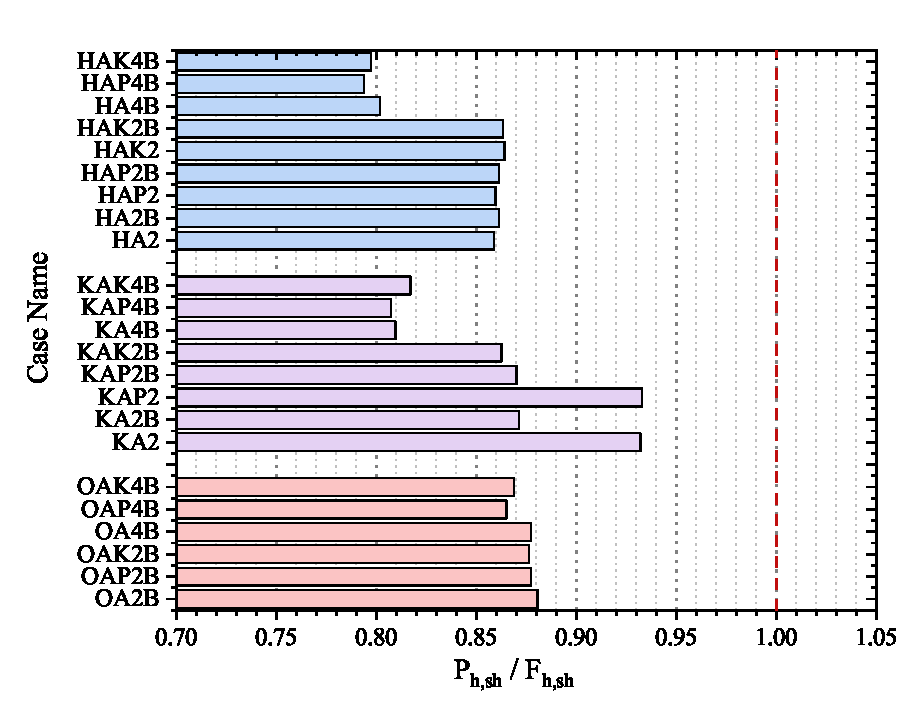
\includegraphics[width=\linewidth]{imgs/ch7/RF-total.eps}
        \caption{Simple accumulate ($F_{h,sh}=F_s+F_b$)}
        \label{fig-fhv}
    \end{subfigure}
    \hfill
    \begin{subfigure}[b]{0.48\textwidth}
        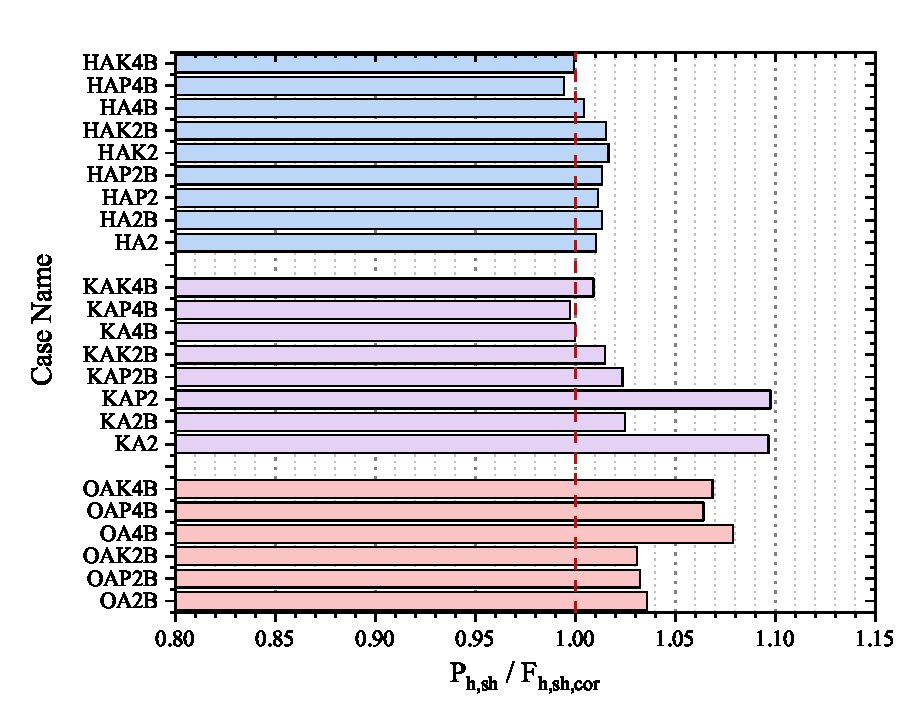
\includegraphics[width=\linewidth]{imgs/ch7/RF-total-cor.eps}
        \caption{After correction - 1 , (Equation \ref{eq-fbh2-1}, Equation \ref{eq-fbh4-1})}
        \label{fig-fhv-cor1}
    \end{subfigure}
    \centering
    \begin{subfigure}[b]{0.48\textwidth}
        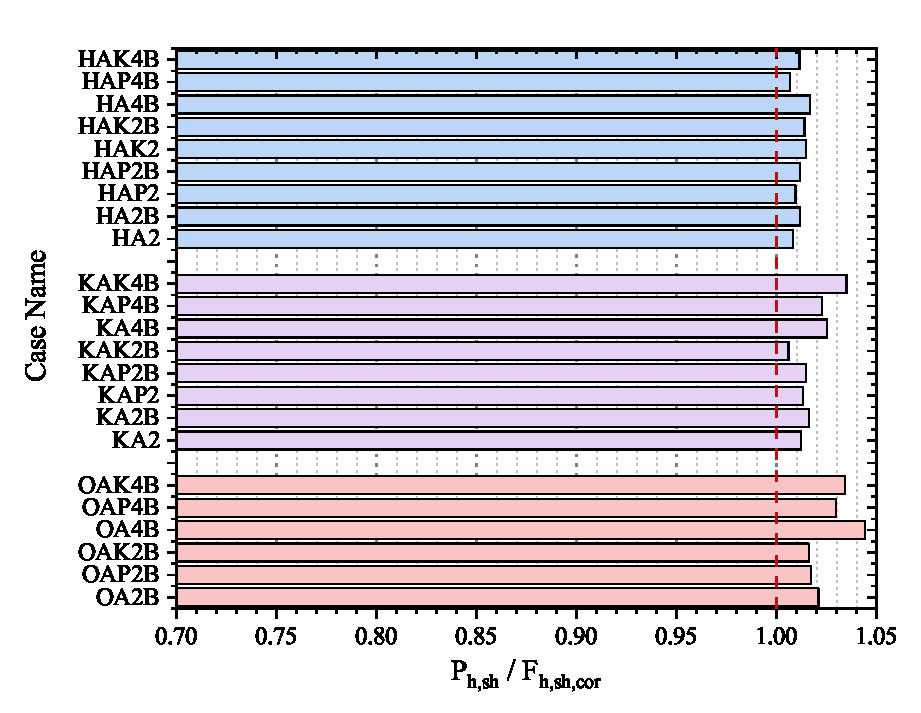
\includegraphics[width=\linewidth]{imgs/ch7/RF-total-cor-2.eps}
        \caption{Correction methods - 2, (Equation \ref{eq-pvh-2})}
        \label{fig-fhv-cor2}
    \end{subfigure}
    \caption{The relationship between analysis value $P_{h,sh}$ and calculated hybrid bolt shank shear yield resistance ($F_{h,sh}, F_{h,sh,cor-1}, F_{h,sh,cor-2}$) of each case}
    \label{fig-fhv-total}
\end{figure*}

Figure \ref{fig-fhv-total} shows the ratio between the analytical result ($P_{h,sh}$) and calculated values ($F_{h,sh}$, $F_{h,sh,cor-1}$, $F_{h,sh,cor-2}$) for each case. The red dashed line represents a ratio of 1 (i.e., the calculated result matches the analytical result). The orange bars represent 12 rows of bolts, the purple bars represent 10 rows of bolts, and the blue bars represent 8 rows of bolts. In figure \ref{fig-fhv}, it can be observed that for the simple accumulate calculation formula $F_{h,sh}$, due to the aforementioned reasons leading to the reduction of friction force and bearing force, the analytical result $P_{h,sh}$ deviates significantly from the calculated value $F_{h,sh}$, and the cases are not well-aligned. 

Figure \ref{fig-fhv-cor1} shows the calculated values obtained by multiplying $F_{sh,h}$ with a correction factor $\alpha_{h,v}$ for the cases with two and four fitted bolts (Equation \ref{eq-fbh2-1}, Equation \ref{eq-fbh4-1}). It can be seen that the analytical result slightly exceeds the calculated values for most cases, but there are a few cases with relatively large deviations, such as the KA2 and KAP2 cases where $\beta_h$ ($F_h/F_y$) is close to 1, or for some cases with 4 fitted bolts where the analytical result are slightly lower than the calculated values, which is not in line with safe design and has poor robustness.

In contrast, figure \ref{fig-fhv-cor2} shows the calculated values obtained by reducing the friction force and bearing force separately (Equation \ref{eq-pvh-2}). It can be observed that the analytical results and calculated values match well, with the analytical results only slightly exceeding the calculated values, which can be considered for safe design. Even in the KA2 and KAP2 cases where $\beta_h$ ($F_h/F_y$) is close to 1, the results are satisfactory, suggesting that this calculation formula is relatively accurate and robust.
%图18显示了了各个case的解析值($P_{hv}$)和计算值($F_{h,sh}, F_{h,sh,cor-1}, F_{h,sh,cor-2}$)的占比关系图. 红色虚线代表解析结果和计算值的比例为1(即计算结果和解析值吻合),橘色bar表示12排螺栓,紫色bar表示10排螺栓,蓝色bar表示8排螺栓。图a中可以发现,对于简单相加的计算公式$F_{h,sh}$,由于上述分析的各种原因导致的摩擦力与承载力的降低,实际的解析结果$P_{h,sh}$与计算值相差较大,且各个case层次不齐。图b展示了在$F_{sh,h}$的基础上分别对两根和四根fit螺栓的情况统一乘上一个矫正系数$\alpha_{h,v}$所获得的计算结果 (Equation \ref{eq-fbh2-1}, Equation \ref{eq-fbh4-1}),可以发现,大部分case的解析值都略微能略微超过计算值,但是极个别的case出现了较大的偏差,例如$\beta_h$ ($F_h/F_y$)很接近1的KA2和KAP2 case,或者对于布置了4根fit螺栓的case,还有个别case略低于计算值,这不符合安全设计,且鲁棒性较差。相比之下,图C展示了分别对摩擦力以及承压力进行折减所获的计算结果 (Equation \ref{eq-pvh-2}),可以发现解析值和计算结果比较吻合,都只略微的超过计算值,超过的部分考虑为安全设计,即使在$\beta_h$ ($F_h/F_y$)很接近1的KA2和KAP2 case中也表现出了不错的结果,可以认为此计算公式较为精确,且鲁棒性好。

Additionally, for figure \ref{fig-fhv-cor2}, it can be observed that for the cases with 4 fitted bolts, the results obtained for 8 rows, 10 rows, and 12 rows differ. The fewer the number of rows (e.g., blue bar, HA case), the closer the result is to the calculated value, and the more rows, the higher the result is compared to the calculated value. This is because the more rows there are, the less impact the loss of friction force due to bearing deformation of the fitted bolts has on the overall reduction rate of the friction force. As shown in Equation \ref{eq-intr-as}, the reduction factor for the friction force is mainly divided into two parts: one is the fitted bolt \#1 at the end, which loses almost all friction force due to deformation, and therefore the friction force of \#1 is not considered, represented by $n_b-1$. The other part is the remaining fitted bolts, whose friction force also experiences an uneven load distribution due to the uneven bearing force, represented by $\alpha_{s,b}$, which is described in detail in Section \ref{sec-rduc-bea}. Therefore, this can explain that if the number of rows increases, $n_s$ will also increase, and the reduction brought by $n_b-1$ and $\alpha_{s,b}$ will be less, resulting in the $P_{h,sh}/F_{h,sh,cor-2}$ for 12 rows (orange bar) being higher relative to 8 rows (blue). The effect of the number of bolt rows (connection length) on the friction force reduction factor will be discussed in the next section.
%另外对于图c,可以发现对于布置了4根fit螺栓的case,8排,10排,12排的情况下获得的结果有所不同,排数越少(蓝色ar,HA case)越接近计算结果,排数越多越高于计算结果,这是由于排数越多,fit螺栓由于承压变形所失去的摩擦力会被其他更多的摩擦型螺栓给缓和掉。如公式2所示,摩擦力的折减因子实际主要分为两个,其中一个是布置在端部\# 1的fit螺栓,由于变形,会失去几乎所有的摩擦力,因此不考虑\# 1 的摩擦力,表示为$n_b-1$,其次,其余的fit螺栓由于承压的载荷分布不均,其分担的摩擦力也会出现载荷分布不均,表示为$\alpha_{s,b}$$,这在第5节进行了详细介绍。因此,这可以解释如果排数越多,那么$n_s$就会越大,$n_b -1$和$\alpha_{s,b}$所带来的折减就越少,因此12排的解析值(橘色)相对于8排(蓝色)会更高。关于螺栓排数(接头长度)带来的对摩擦力折减系数的影响,在下一节会稍作讨论。

\begin{equation}
    \alpha_s F_s \approx ((n_s+ (n_b-1)\alpha_{s,b}) F_{s1} ) 
    \label{eq-intr-as}
\end{equation}


\subsection{Reduction of joint length}

\begin{figure}
    \centering
    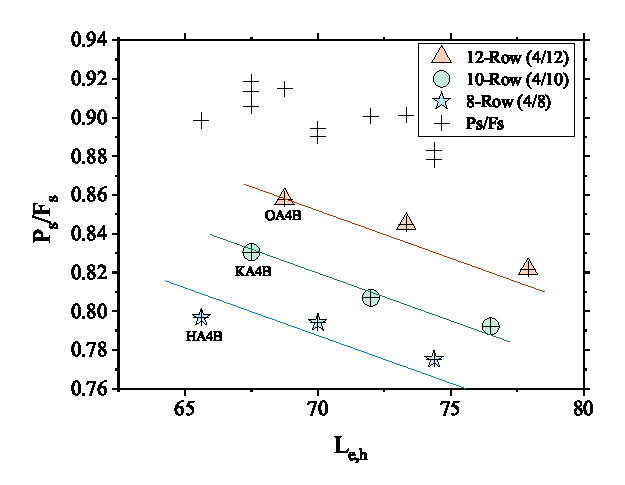
\includegraphics[width=\linewidth]{imgs/ch7/as-leh.eps}
    \caption{ $\alpha_s ((P_b-P_{b,\#1})/((n_b)F_{shy1})$ and effective joint length $L_{e,h}$}
    \label{fig-rdc-leh}
\end{figure}

Figure \ref{fig-rdc-leh} shows the relationship between the friction force reduction rate and the effective length of the combined connection, $L_{e,h}$ (non-dimensionalized by the number of bolt rows, $L_{e,h} = L_J / n_b$). The coloured plots represent the cases with 4 fitted bolts, where the orange triangles represent 12 rows of bolts, the green circles represent 10 rows of bolts, and the blue triangles represent 8 rows of bolts. In figure \ref{fig-rdc-leh}, it can be observed that for the cases with 4 fitted bolts, as the joint effective length increases, the friction force reduction rate decreases. For the cases with 2 fitted bolts (represented by the + symbol), no obvious relationship between the friction force reduction rate and the joint effective length is found. 
%Figure \ref{fig-av-leh} shows that when the friction force of the end fitted bolt \# 1 is ignored, the R-square value for the relationship between the friction force reduction rate $\alpha_{sb}$ of the other fitted bolts and the joint effective length is 0.5, indicating a moderate linear relationship, although not strong. The investigation of the relationship between the effective length of the connection and the friction force reduction rate will be further discussed as a technical problem.
%图20显示了摩擦力的降低率和混合接头有效长的关系,混合接头有效长度 $L_{e,h}$ (对螺栓排数进行无量纲化,$L_{e,h} = L_J / n_b$)。着色的plot为配置了4根fit螺栓的case,其中橙色的三角形代表了12排螺栓,绿色的圆形代表了10排螺栓,蓝色三角形代表了8排螺栓。图a中可以发现,配置了4根fit螺栓的case随着接头的有效长度的增加摩擦力的减少率降低,对于配置了2根fit螺栓的case($+$ 记号),没有发现摩擦力减少率和接头有效长度存在明显的关系。
%图b显示了当忽略掉端部\#1 fit螺栓的摩擦力时,基于其他fit螺栓的摩擦力减少率$\alpha_{sb}$和接头的有效长度的R-square为0.5,可以说明虽然不强,但表现出了一定程度的线性关系,对于接头有效长度和摩擦力降低率的探讨将作为今后的课题继续讨论。

\begin{equation} \label{eq-asb}
    \alpha_{sb}=(P_{s,b}-P_{s,b-\#1})/((n_b-1) F_{s1})
\end{equation}

%%%%%%%%%%%%%%%%%%%%%%%%%%%%%%%%%%%%%%%%%%%%%%%%%%%%%





\section{SLS for hybrid connection}

According to the numerical analysis in the previous section and the comparison with the experimental results, although JSHB follows the formula $1.7f_y$ for the design of the \ac{ASD} methods, it can be found that this formula is too high for evaluating the limit state of the use of the bearing connection, especially for the hybrid joint, the bearing connection always has to share more force than the general bolts, so for the design of bearing resistance for the hybrid connection, the present study concludes that It is more reliable to cancel the coefficient before yield strength, and the design formula for bearing yield resistance for one fastener $F_{by1}$ is as follows:

\begin{equation}
    F_{by1} = dtf_y
\end{equation}

In this study, it is considered that the bearing connection in the use of limit state in addition to the bearing yield will also appear fastener shear yield, fastener shear yield for one fastener $F_{vy1}$ can be calculated by the following formula to obtain.

\begin{equation}
    F_{vy1} = A_s f_{yb}/\sqrt{3}
\end{equation}

the slip resistance per fastener shall taken as:

\begin{equation}
    F_{s1} = m \mu N_0
\end{equation}


For the resistance of hybrid joints, this study suggests that the resistance of a hybrid joint can be obtained directly by adding the smaller of the bearing yield resistance and the shear yield resistance of the person and the slip resistance, however, this is only the ideal state, and the actual strength will be affected by the following two main aspects, 1. Slip resistance attenuation of Kinetic friction $\alpha_{kf}$, 2. reduction of bolt preload due to bolt was under shear yield $\alpha_{v}$, and 3. Friction/bearing load sharing mechanism $\beta_{ls}$. These two factors primarily determine the magnitude of slip strength and bearing resistance when added together. Preliminarily, this can be calculated by the following formula:

For bolt shear yield resistance:

\begin{equation}
    F_{hv} = (n_f + \alpha_{v}(n_b-1)) F_s + \beta_{ls} n_b F_{vy})
\end{equation}

For bearing yield resistance:

\begin{equation}
    F_{hb} = n F_s + \beta_{ls} n_b F_{by}
\end{equation}

Where, $\alpha_{kf}$ is attenuation factor for kinetic friction, $\alpha_v$ is Correction factor for loss of preload due to shear failure, $\beta_{ls}$ is the correction factor for load sharing. $n$ is the number of the fastener, $n_f$ is the number of the fastener for friction type connections, $n_b$ is the number of the fastener for bearing type connections.

\subsection{Fastener shear yield}

In the bearing type connection, for the serviceability limit state, can be divided into two kinds, one is the fastener shear yield, the other is the bearing yield of the main plate, although the two kinds are one of the bearing limit state, in order to facilitate the calculation as well as to facilitate the differentiation, here will be the two kinds of limit state are discussed separately, and each of them has a different mechanical behavior.

Table \ref{tabfe-shfst} lists the geometric information for this resolved case as well as the material and contact properties used. Table \ref{tabjr-sfst} lists the calculated resistance of the hybrid joints.

\begin{table}[htbp]
\centering
\caption{Various property for FE analysis}\label{tabfe-shfst}
\begin{tabular}{@{}cccccccccc@{}}
\toprule
 &
  \begin{tabular}[c]{@{}c@{}}$w$\\ {[}mm{]}\end{tabular} &
  \begin{tabular}[c]{@{}c@{}}$t$\\ {[}mm{]}\end{tabular} &
  \begin{tabular}[c]{@{}c@{}}$d_0$\\ {[}mm{]}\end{tabular} &
  \begin{tabular}[c]{@{}c@{}}Number of\\ bolt\end{tabular} &
  \begin{tabular}[c]{@{}c@{}}Bolt for \\ bearing\end{tabular} &
  $\mu$ &
  \begin{tabular}[c]{@{}c@{}}$N_0$\\ {[}kN{]}\end{tabular} &
  \begin{tabular}[c]{@{}c@{}}$f_y$\\ {[}Mpa{]}\end{tabular} &
  \begin{tabular}[c]{@{}c@{}}$f_u$\\ {[}Mpa{]}\end{tabular} \\ \midrule
shear-fst &
  210 &
  50 &
  18 &
  10 &
  4 &
  0.4 &
  106 &
  550 &
  694 \\ \bottomrule
\end{tabular}
\end{table}


\begin{table}[htbp]
\centering
\caption{Summary of joint resistance (unit: kN)}\label{tabjr-sfst}
\begin{tabular}{@{}ccccccccc@{}}
\toprule
 &
  \multicolumn{5}{c|}{SLS} &
  \multicolumn{3}{c}{ULS} \\ \midrule
 &
  \begin{tabular}[c]{@{}c@{}}$F_s$\end{tabular} &
  \begin{tabular}[c]{@{}c@{}}$F_{by}$\end{tabular} &
  \begin{tabular}[c]{@{}c@{}}$F_{vy}$\end{tabular} &
  \begin{tabular}[c]{@{}c@{}}$F_h$\end{tabular} &
  \multicolumn{1}{c|}{\begin{tabular}[c]{@{}c@{}}$F_y$ \end{tabular}} &
  \begin{tabular}[c]{@{}c@{}}$F_b$\end{tabular} &
  \begin{tabular}[c]{@{}c@{}}$F_v$\end{tabular} &
  \begin{tabular}[c]{@{}c@{}}$F_u$\end{tabular} \\ \cmidrule(l){2-9} 
shear yield &
  848 &
  1760 &
  835 &
  1438 &
  5280 &
  
  5552 &
  2320 &
  6697 \\ \bottomrule
\end{tabular}
\end{table}


Fig. \ref{fig-beafst} shows the The relationship between load and relative displacement when shear yield first case occurs. After the fastener shaft shear yielding occurred, two more slope changes occurred with a slight increase in slope due to the fact that on two separate occasions, the main plate bore wall contacted the bolt shaft used for the friction connection, and as the displacement continued to occur, the third time the slope changed to the contact between the connection plate and the fastener shaft. From this point on the connection forms a fully bearing type connection.

\begin{figure}[htbp]
    \centering
    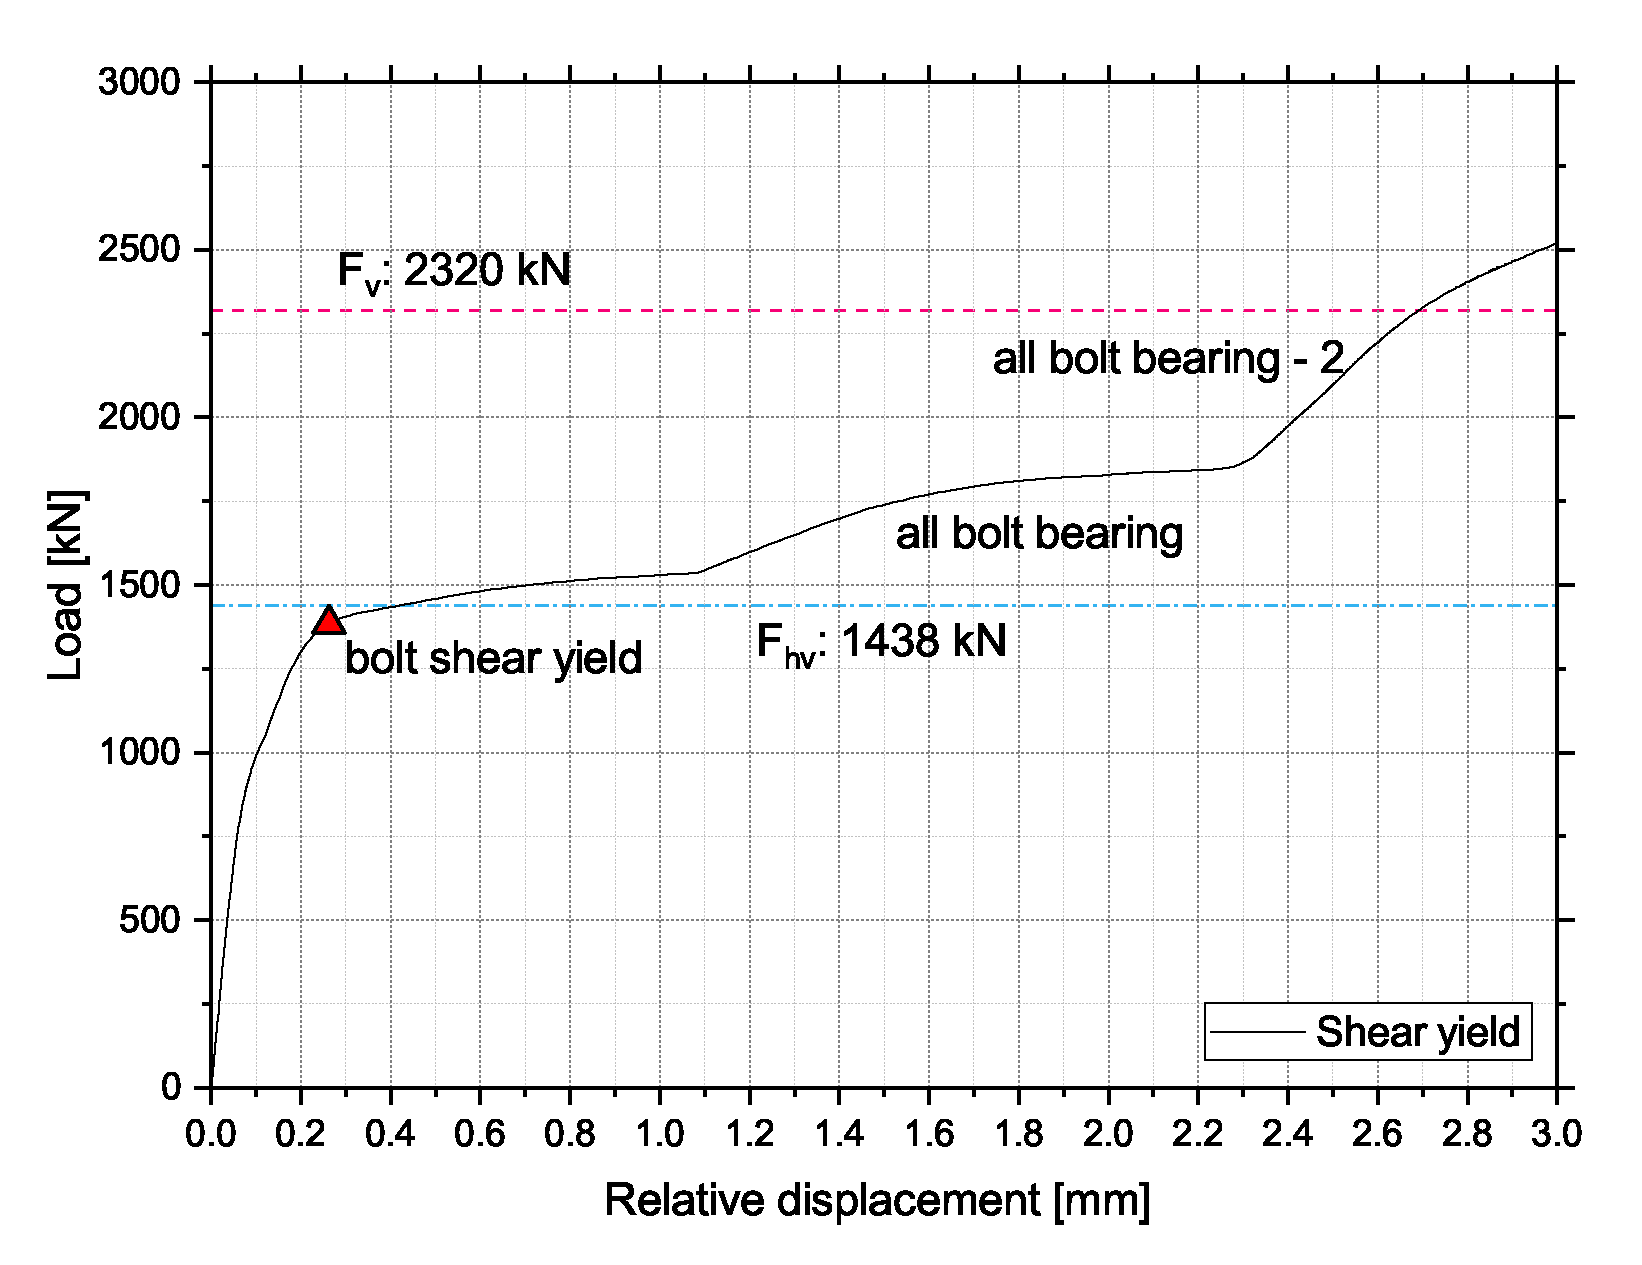
\includegraphics[width=0.8\textwidth]{imgs/ch7/M16b4-2.eps}
    \caption{The relationship between load and relative displacement}
    \label{fig-m16b4}
\end{figure}

Fig. \ref{fig-m16b4fvf} shows the Mises stress counter, from the figure can be found in the load of 1106kn, located in the end of the bolt in the shear surface occurred in the full cross-section yielding this and the curve occurred in the nonlinear (that is, the labeled point) position is approximately the same, which shows that the curve of the nonlinear behavior of the bolt by the shear yielding, and therefore can be considered to be the use of the bolt yielding the bolt of the limit state of hybrid joints

\begin{figure}[htbp]
    \centering
    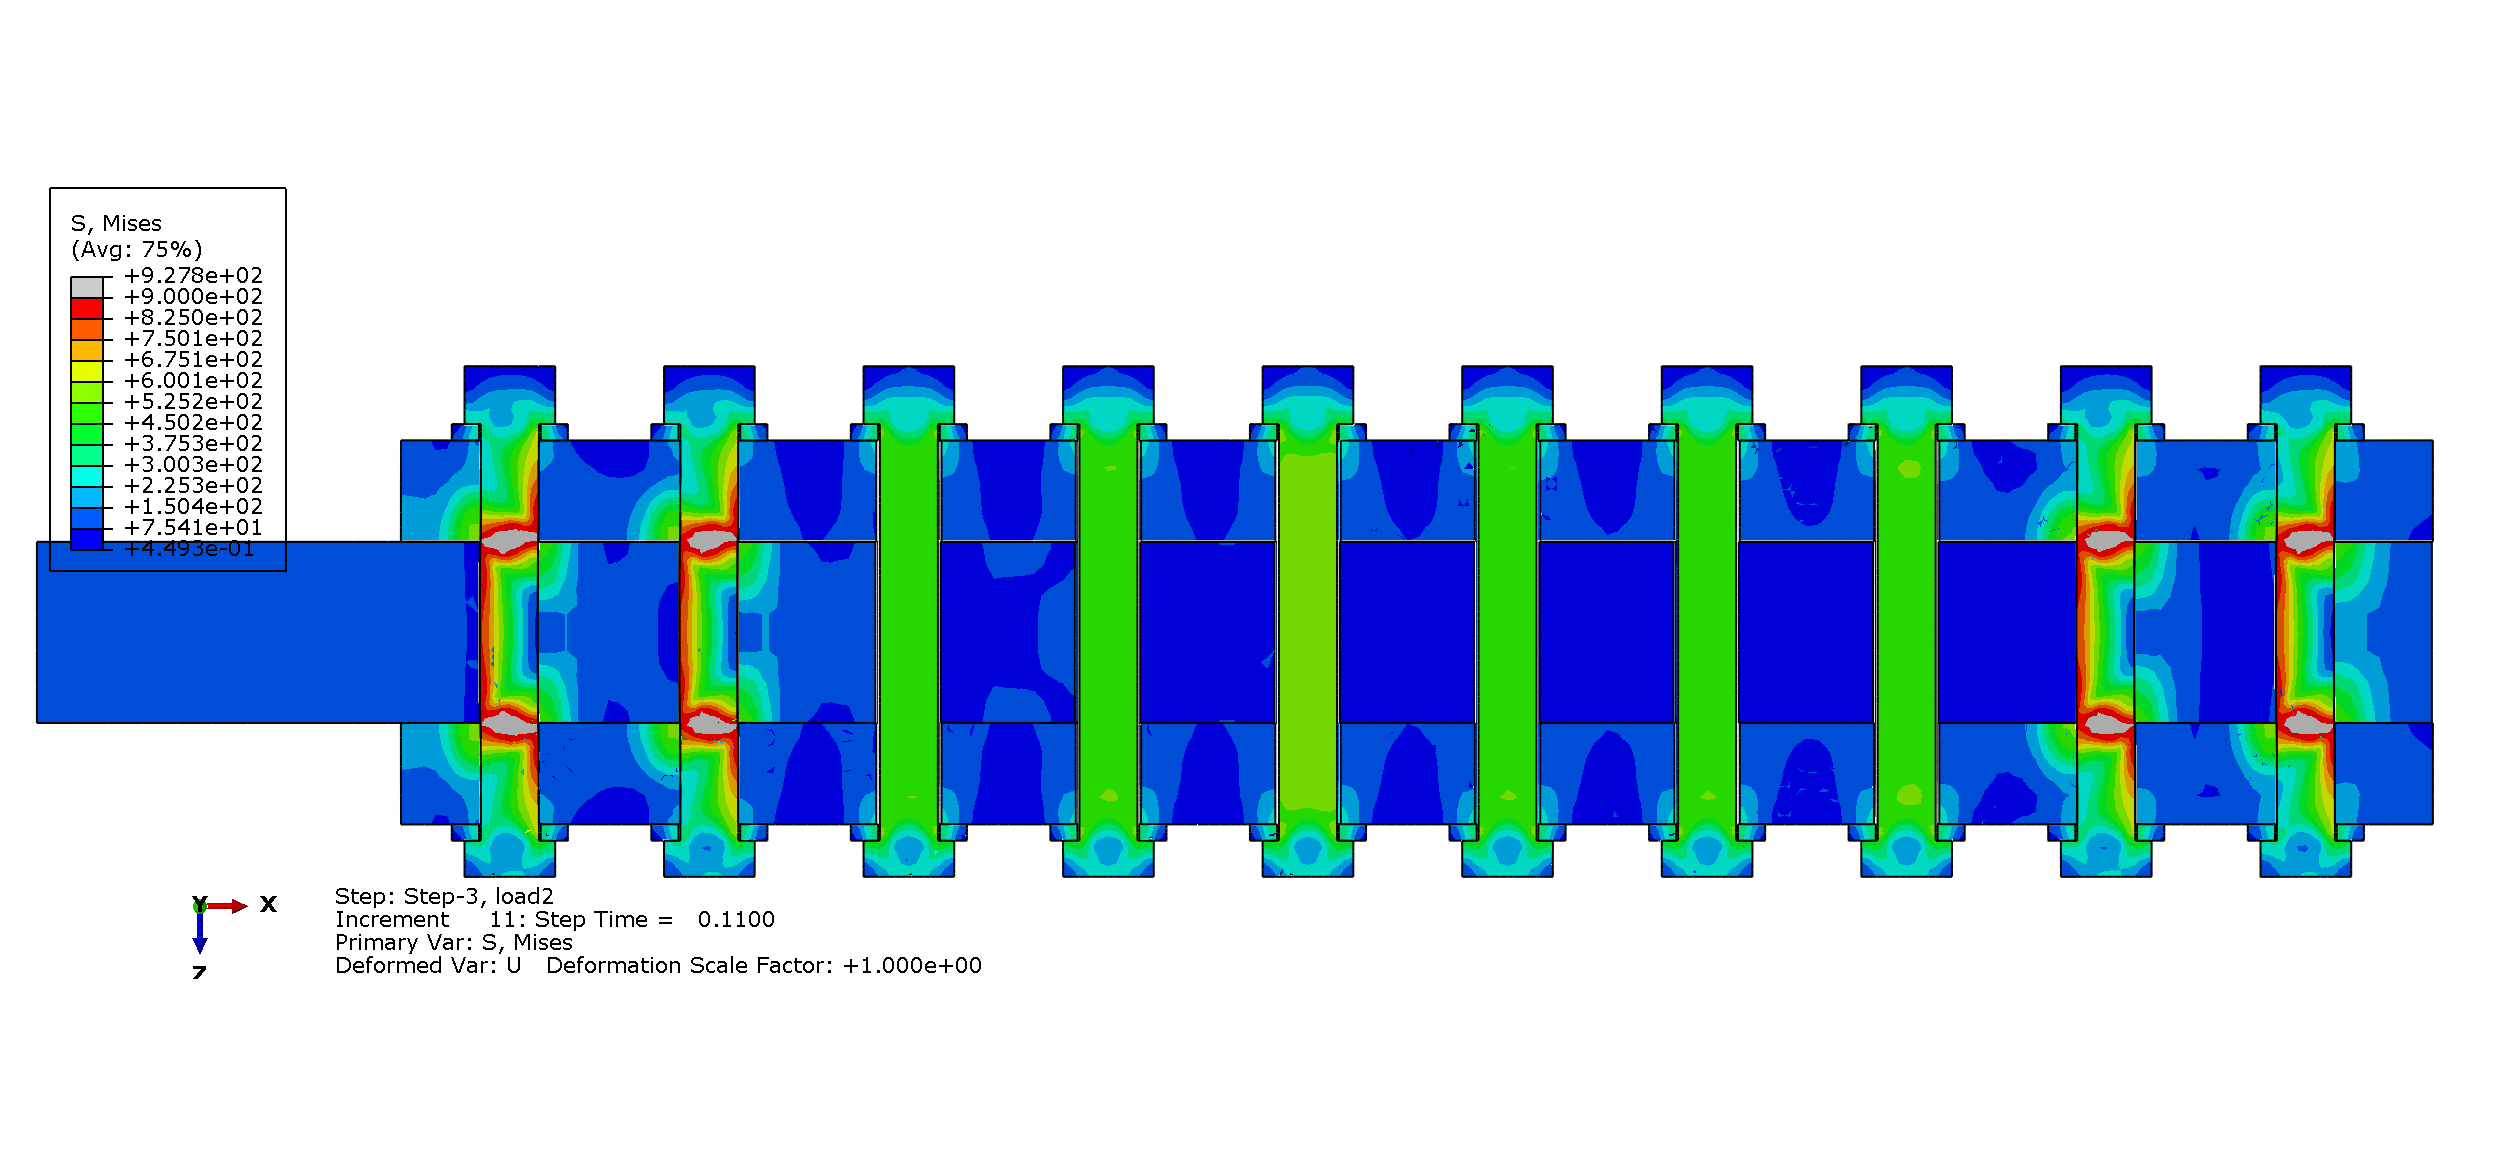
\includegraphics[width=0.8\textwidth]{imgs/ch7/M16b4-fvfst.png}
    \caption{The fastener shear yield was occurred when load is equal to the 1384 kN}
    \label{fig-m16b4fvf}
\end{figure}


\subsubsection{Reduction factor for bolt preload}

%图1表示了当发生了螺栓截面剪切屈服时,螺栓轴力的降低情况。可以发现受剪切屈服的影响,端部用于承压连接的螺栓的轴力相对于中间的用于摩擦连接的螺栓的轴力的降低情况要大很多,端部4个螺栓的平均下降率低至0.76,也就是说用于承压连接的螺栓来说,当受到剪切屈服的影响时,轴力平均会下降至0.76,这个系数可以直接用于基于用于承压连接螺栓的折减系数。也可以对对于螺栓整体数量来进行折减,对于整体来说降低率为0.89(等效降低率).
Fig. \ref{fig-b4ls} shows the reduction of the bolt preload when shear yielding of the bolt section occurs. It can be found that by the effect of shear yielding, the reduction of the preload of the bolts used for bearing connection at the end is much larger compared to the reduction of the preload of the bolts used for friction connection in the middle, and the average rate of reduction of the four bolts at the end is as low as 0.76, which means that for the bolts used for bearing connection, the preload decreases to an average of 0.76 when it is subjected to the effect of shear yielding, and this coefficient can be used directly for the reduction coefficient based on the bolts used for This coefficient can be directly used as a reduction factor for bolts used in connections under bearing pressure. This factor can be used directly for the reduction factor based on the number of bolts in the pressurized connection. It is also possible to reduce the number of bolts as a whole, with an overall reduction $\alpha_v$ of 0.89 (equivalent reduction rate).

\begin{figure}[htbp]
    \centering
    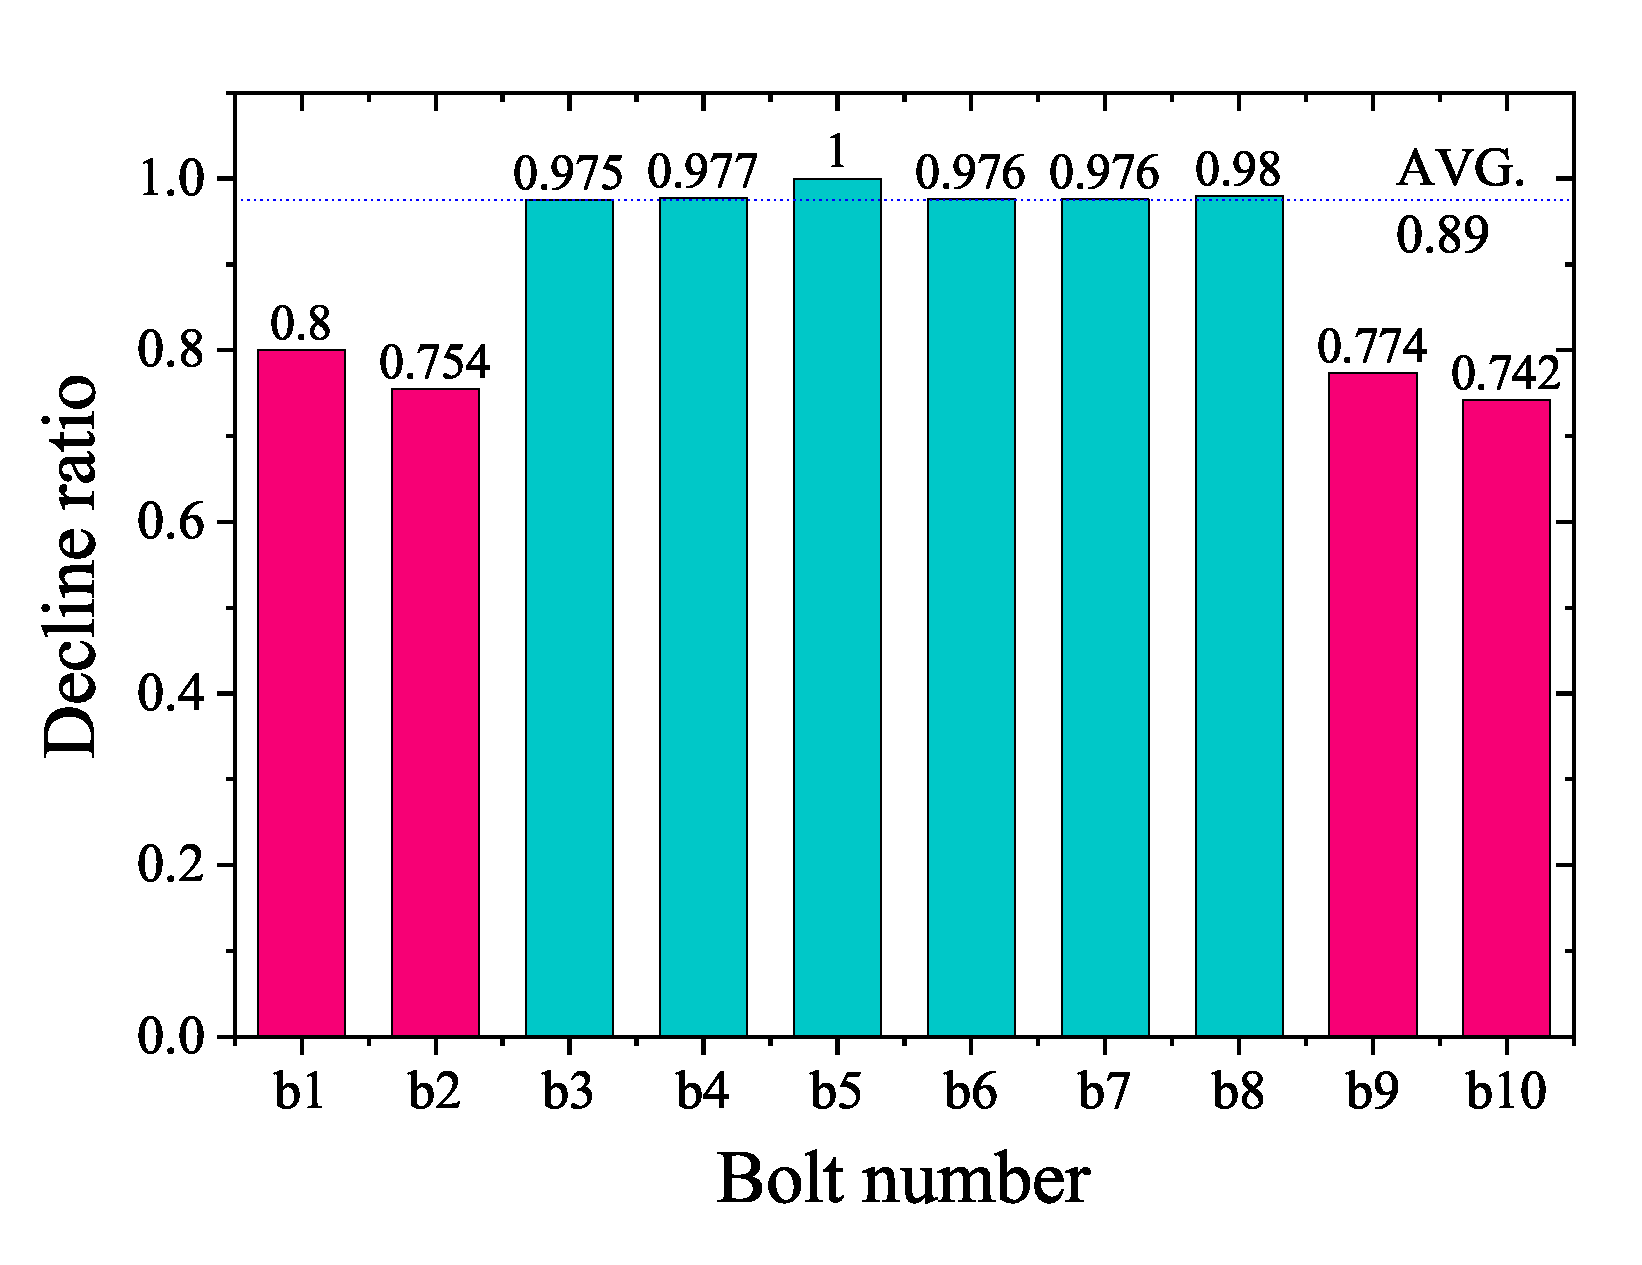
\includegraphics[width=0.7\textwidth]{imgs/ch7/b4-ls.eps}
    \caption{Decline ratio of bolt preload when load is equal to the 1384 kN}
    \label{fig-b4ls}
\end{figure}

\subsubsection{Reduction factor for front end fastener}

Fig. \ref{fig-cstavfst} shows the CSTATUS counter when load is 1384 kN,Fig. \ref{fig-cstavfst} Deformation of z direction counter when load is 1384 kN.
It can be observed that although the No.1 bolt at the end has residual axial force, due to the out-of-plane deformation of the connection plate (see Fig. \ref{fig-cstavfst}), most of the contact range of the \#1 bolt (b1) has completely changed from the original slipping state to the state of not in contact (see Fig. \ref{fig-cstavfst}), that is to say, in this area, the contact pressure is lost, resulting in friction failure, and therefore it is considered that the No.1 bolt at the end is not in contact. Friction and bearing pressure cannot work together when bearing pressure. When calculating the friction strength, n should be subtracted from 1.

\begin{figure}[htbp]
    \centering
    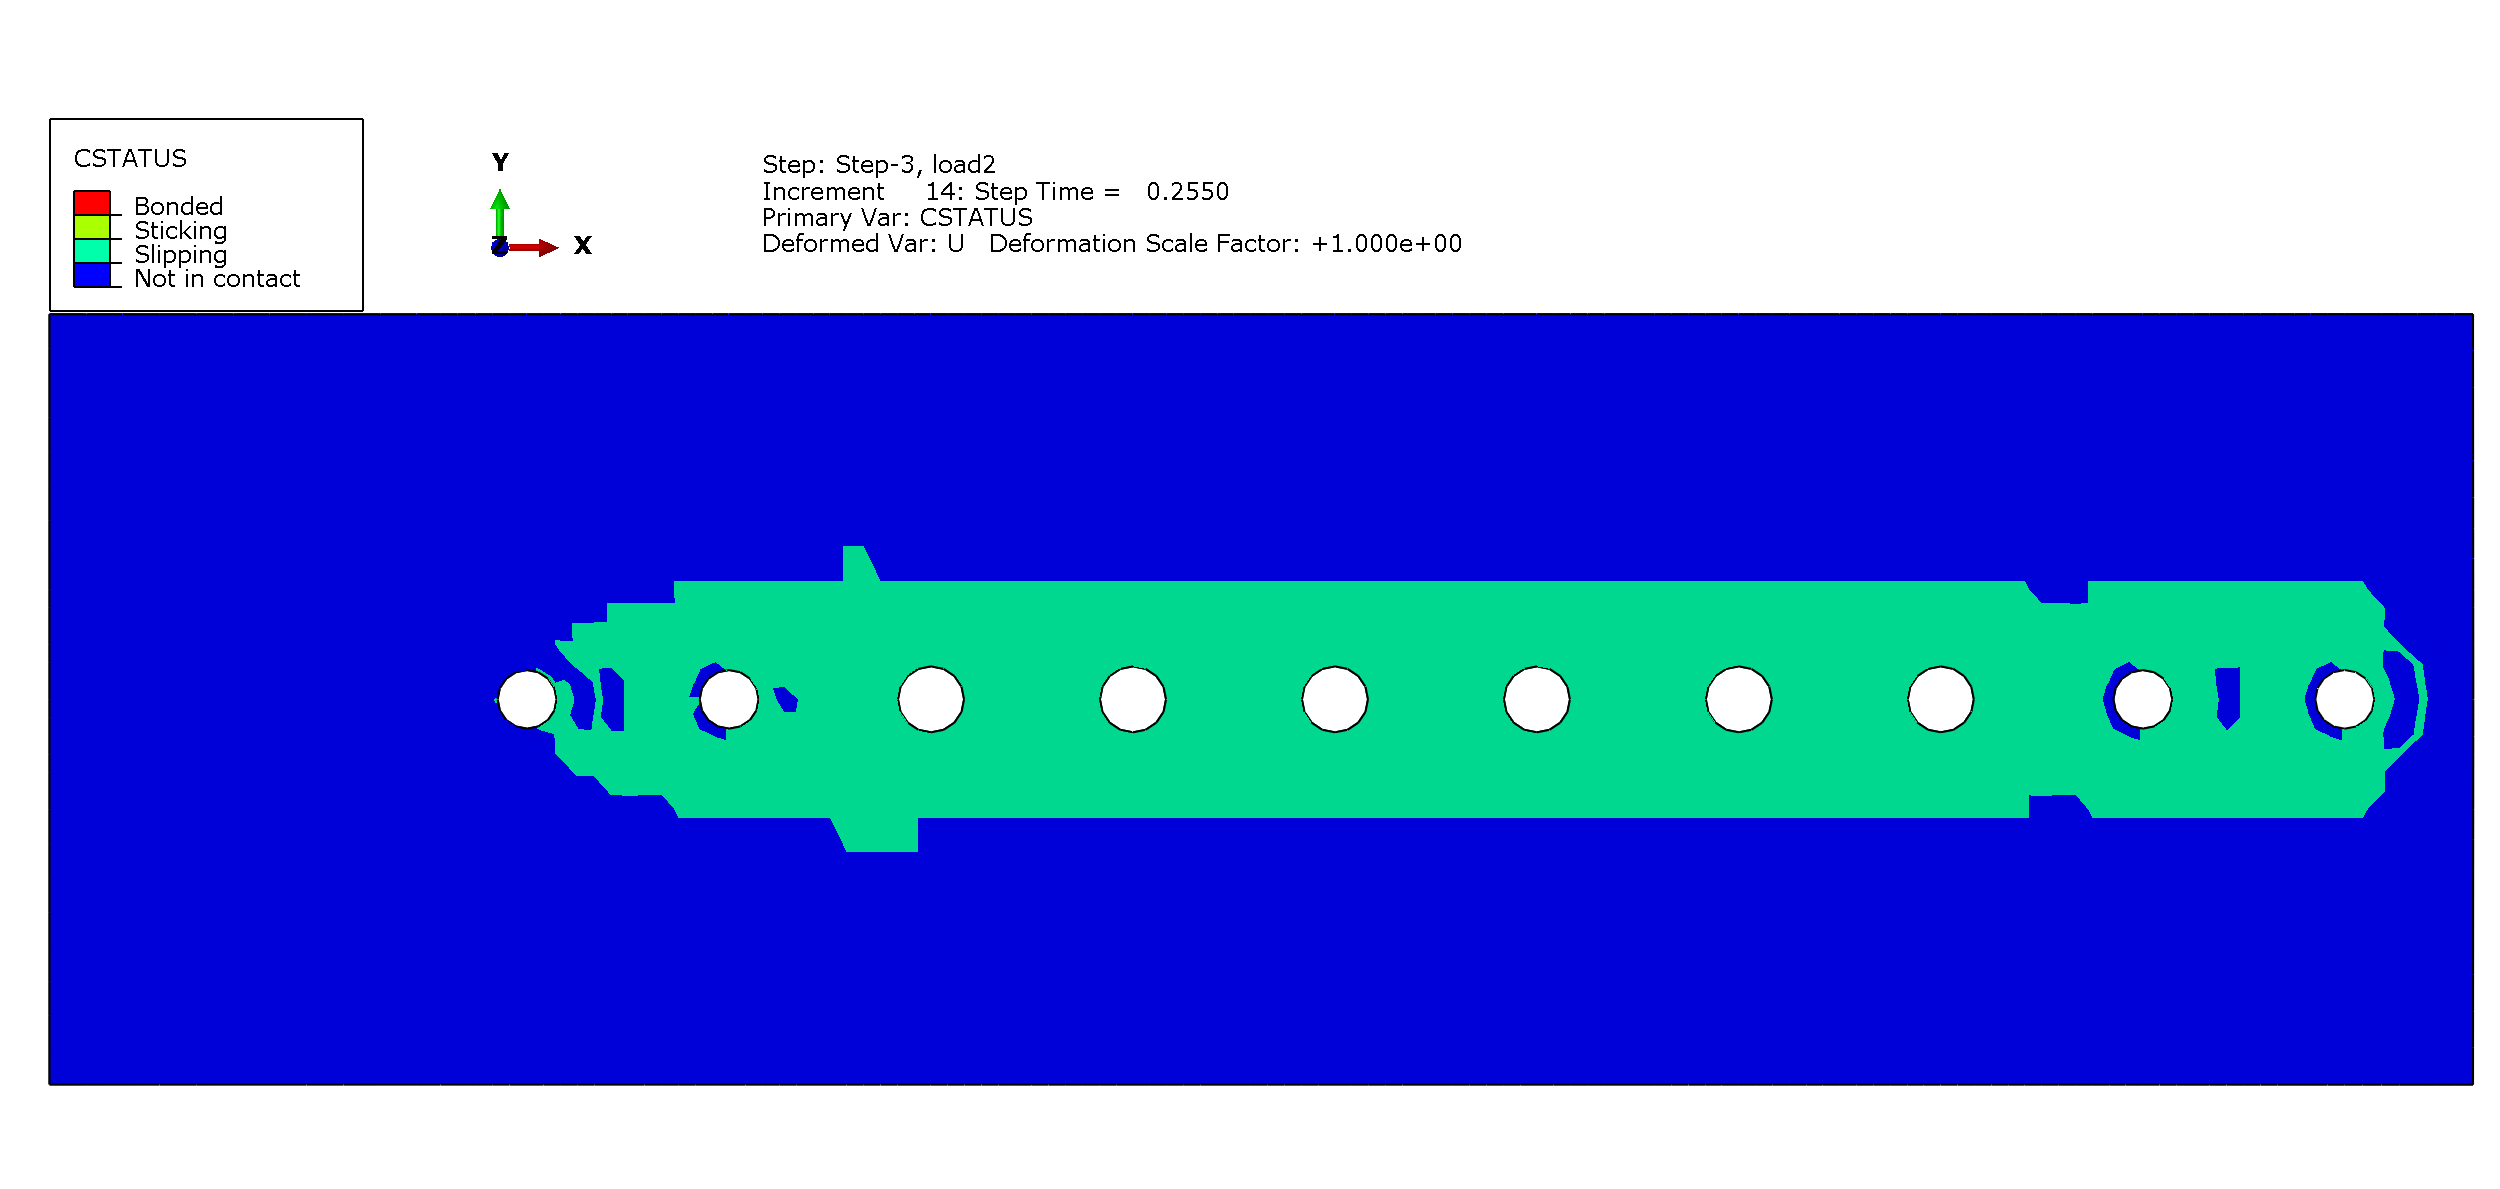
\includegraphics[width=0.8\textwidth]{imgs/ch7/cstatus-vfst.png}
    \caption{CSTATUS counter when load is 1384 kN}
    \label{fig-cstavfst}
\end{figure}

\begin{figure}[htbp]
    \centering
    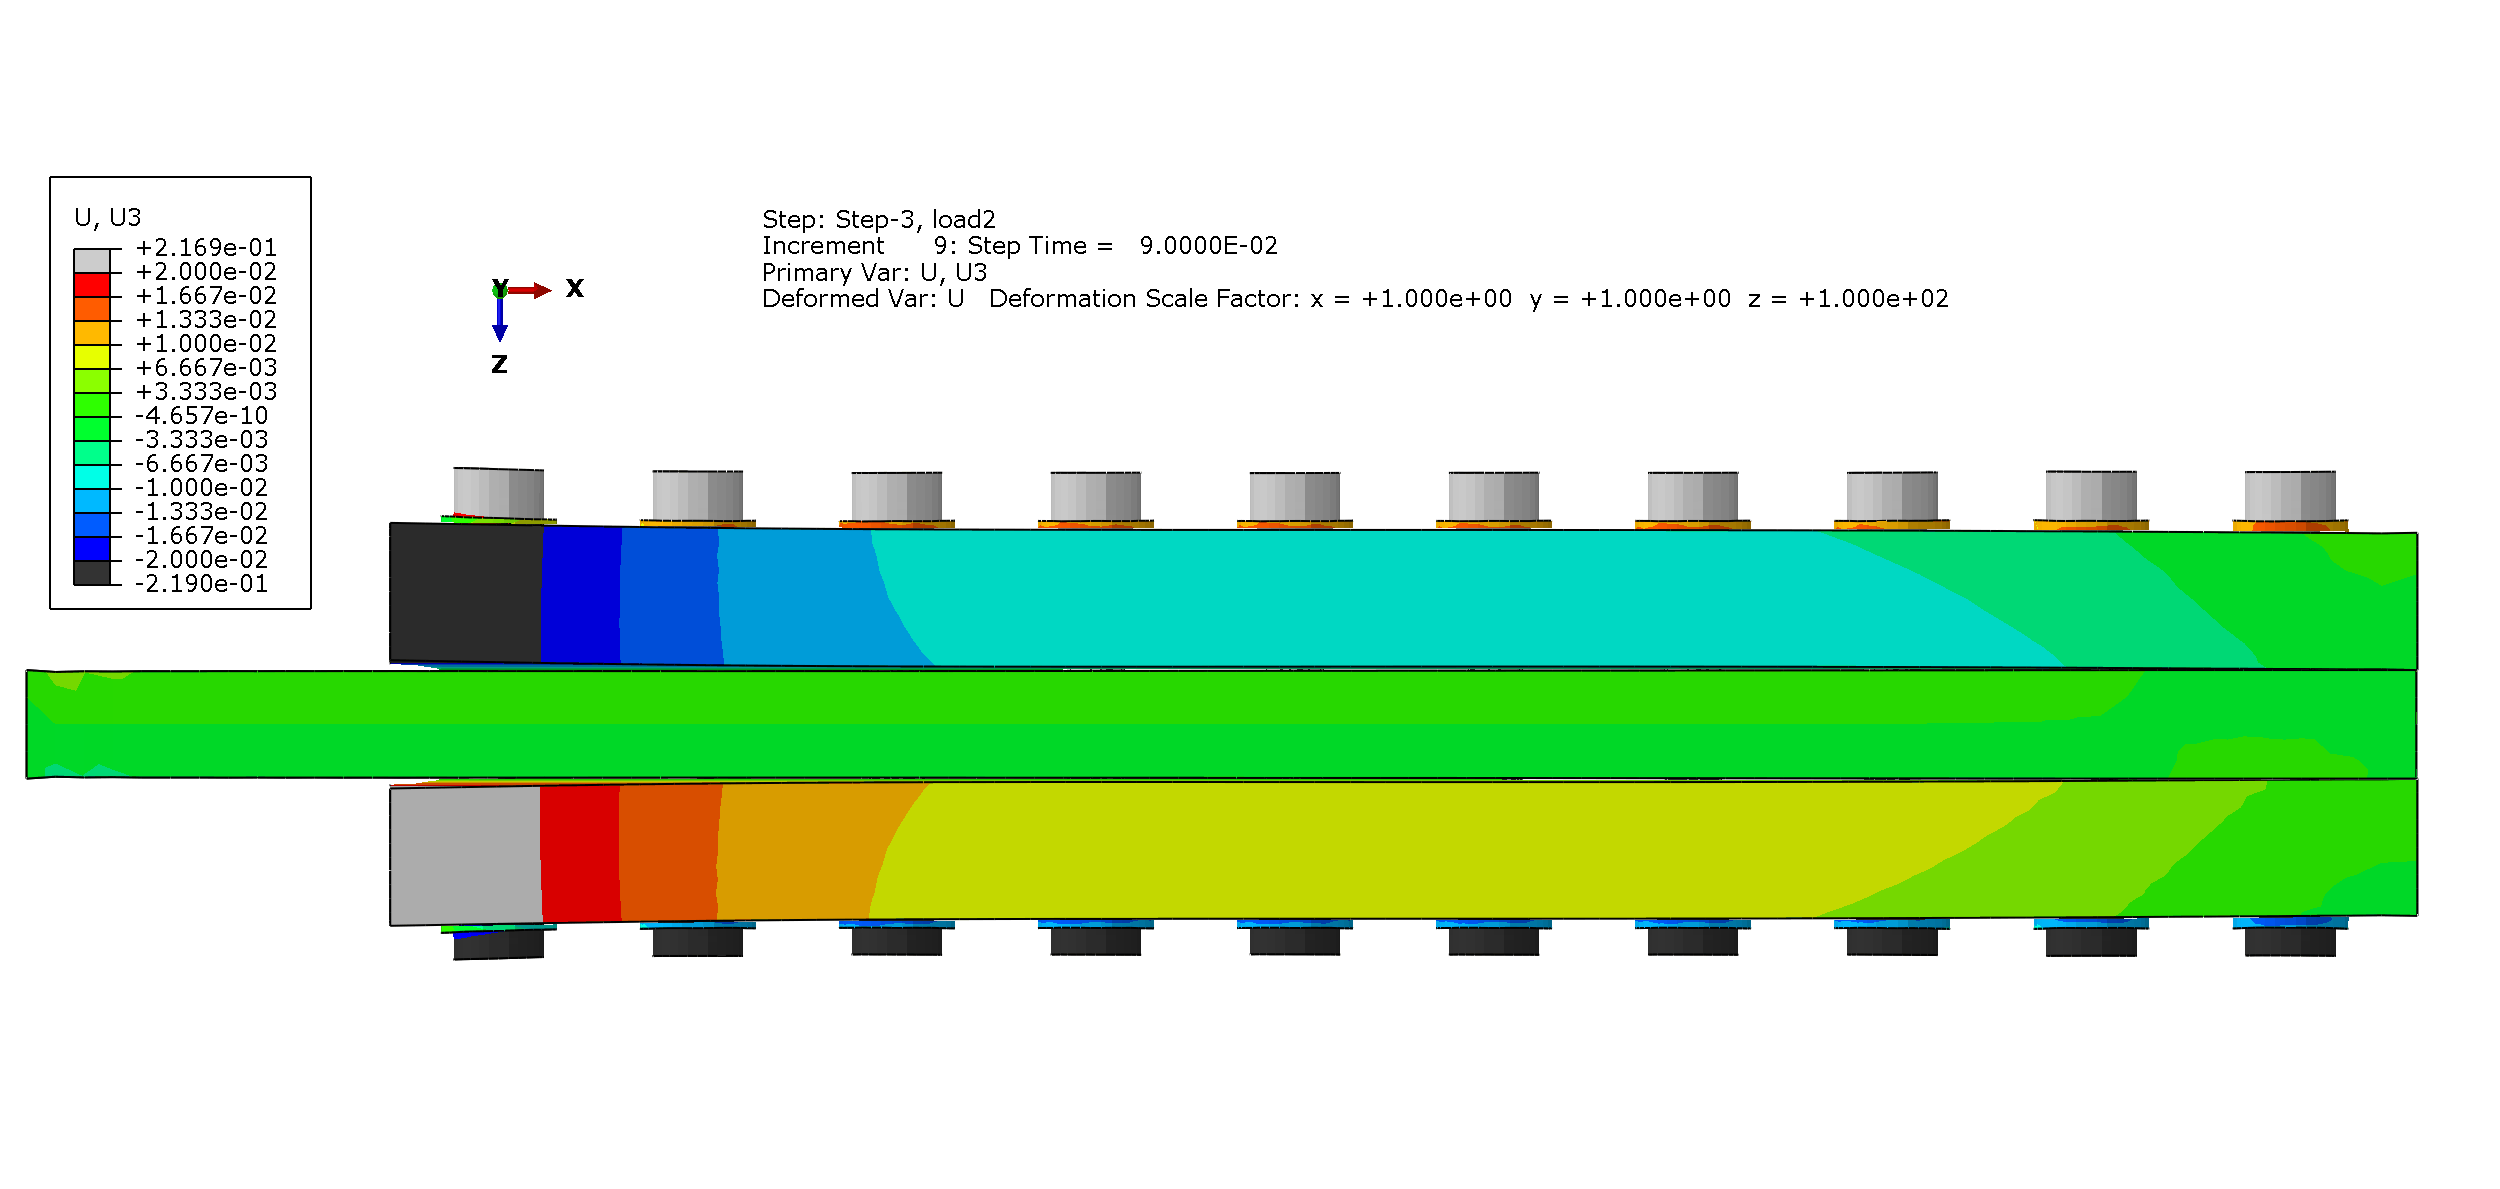
\includegraphics[width=0.8\textwidth]{imgs/ch7/U3-vfst.png}
    \caption{Deformation of Z (U3) direction counter when load is 1384 kN}
    \label{fig-u3vfst}
\end{figure}


Fig. \ref{fig-bcsche} shows the Boundary conditions and deformation schematic, The cross-sectional force acting on the main plate is divided into the cross-sectional forces of the main plate and splice plate via the shear transmit on the bolt. Assuming that the point of action of each cross-sectional force is at the center of the plate, an additional bending moment is generated in the bolt due to the eccentricity of the cross-sectional forces. The boundary condition at the end of the connection plate is free, so there is a tendency to deform outward toward the main plate faying surface when subjected to additional bending moments, resulting in a separation of the connection plate from the main plate, and therefore a loss of friction force.

\begin{figure}[htbp]
    \centering
    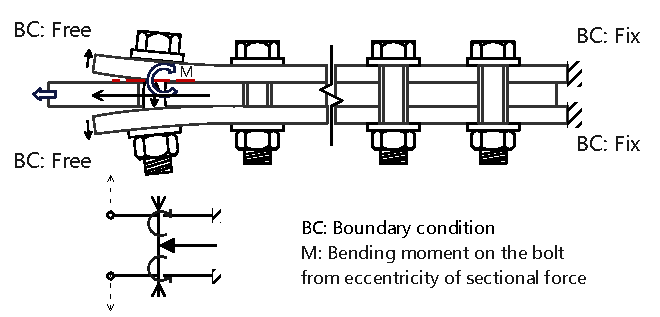
\includegraphics[width=0.9\textwidth]{imgs/ch7/bcschema.pdf}
    \caption{Schematic of the boundary conditions and deformation}
    \label{fig-bcsche}
\end{figure}


\subsubsection{Reduction factor for unevenly load sharing}

Uneven load distribution in a bearing connection can cause a particular fastener to reach the specified strength before another, the load distribution can be seen in Fig. \ref{fig-bshare} in Chapter \ref{ch5}. In addition, due to the decrease in friction in a bearing connection, it returns to share more bearing pressure than expected, which can cause this fastener to reach a yield state more quickly. Based on the data from the FE analysis in Chapter \ref{ch5}, the correction factor due to the load sharing $\beta_{ls}$ is taken to be 0.9.

Fig. \ref{fig-beals-b4} shows the distribution of bearing forces on individual bolts for this analysis (when the shear gross section of the bolt shaft yields, i.e., 1384 kN), and again it can be seen that the fasteners are not uniformly stressed.

\begin{figure}[htbp]
    \centering
    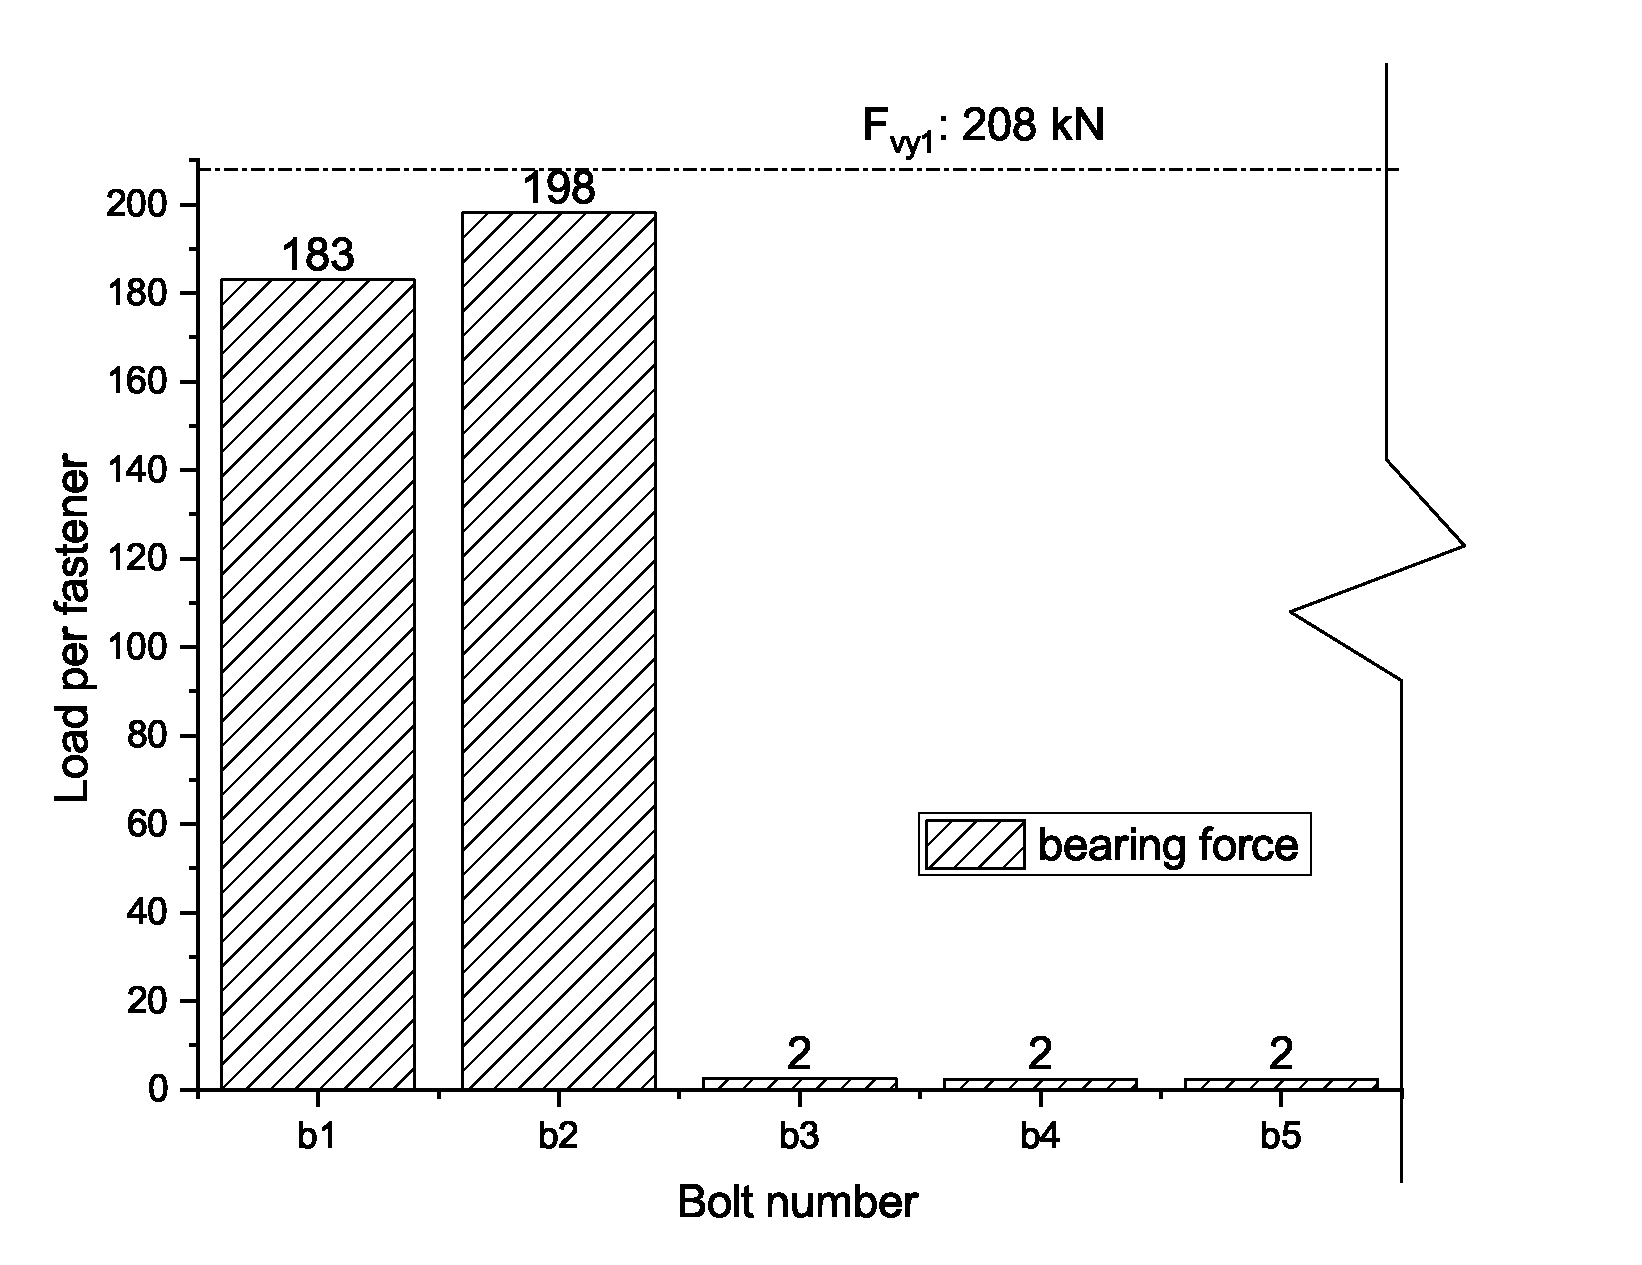
\includegraphics[width=0.7\textwidth]{imgs/ch7/beals-b4.eps}
    \caption{the distribution of bearing forces on individual bolts for this analysis (when the shear gross section of the bolt shaft yields, i.e., 1384 kN)}
    \label{fig-beals-b4}
\end{figure}

In addition, fasteners at the ends are always more affected by deformation than those measured internally due to the difference in boundary conditions. That is, at the front end of the joint, the connection plate is free while the main plate is fixed, so when loaded, the connection plate will always have a tendency to bend outward toward the face, which will exacerbate the deformation of the bolt. Therefore, this is one of the reasons for the uneven force on the end bolts.


\subsubsection{Summary}

For the shear yield strength of bolts, since the preload is significantly reduced when the shear surface of the bolt is plastically expanded, the immediate effect is the loss of the friction it bears, which can result in a reduction in friction $\alpha_{v}$. In addition, for the hybrid connection configured with bearing type connection at the end only, the bearing type connection at the end is affected by the uneven load distribution, the bolt subjected to more force is 1.2 times higher than the bolt subjected to less force, so for the sake of convenience of calculation, $\beta_{ls} = 0.9 $ is taken as the phenomenon of individual bolts subjected to too much load due to the uneven distribution of the load, which leads to the phenomenon of yield first, and this is also valid for the bearing yielding state.

In addition, if there is a fastener for bearing type connection located at the front end, its friction will cause deformation of the main plate due to bending moment generated by shear, which will result in the loss of friction, so it is recommended that the friction of the front end (b1) bolt be ignored in such cases.

For SLS :
if bearing type connection is arranged at the front end of the joint :

\begin{equation}
\begin{aligned}
    F_{hv} &= (n_f+ \alpha_v(n_b-1)) F_s + \beta_{ls} n_b F_{vy1} \\
           &= (n_f + 0.7(n_b-1)) F_{s1} + 0.9 n_b F_{vy1}
\end{aligned}
\end{equation}

if not:

\begin{equation}
\begin{aligned}
    F_{hv} &= (n_f+ \alpha_v n_b) F_s + \beta_{ls} n_b F_{vy1} \\
           &= (n_f + 0.7 n_b) F_{s1} + 0.9 n_b F_{vy1}
\end{aligned}
\end{equation}

Summarizing with the above discussion, the two complementary coefficients can be respectively $\alpha_v = 0.75 \approx 0.7$, $\beta_{ls} = 0.9$

For the maximum resistance due to bolt shear, although there will always be residual friction that will participate in the transfer of the load together until the maximum load is reached, however, since this is considered unreliable, the friction due to the preloading of the bolt is usually not taken into account in the calculation of the ultimate resistance. The same is true for hybrid joints, so for the design of the ultimate shear strength of hybrid joints, the calculation is normalized according to the following equation.

For ULS:

% \begin{equation}
%     F_v = \beta_{ls} n A_s f_{ub}
% \end{equation}
\begin{equation}
    F_v = n A_s f_{ub}
\end{equation}

\subsection{Bearing yield of the main plate}

Hybrid connection bearing yielding mainly confirms the fastener holes of the bearing type connection, in Chapter \ref{ch4} mainly discusses the judgment of bearing yielding, for any fastener holes around the hole including to the direction of the plate thickness has reached the equivalent diameter range of the plastic region, the judgment of fastener holes bearing yielding occurs. Specific judgment can be referred to in Chapter \ref{ch4}, followed by a simple use of stress maps to describe the stress characteristics of bearing yielding.

Table \ref{tabfe-beafst} lists the geometric information for this resolved case as well as the material and contact properties used. Table \ref{tabjr-bfst} lists the calculated resistance of the hybrid joints.

\begin{table}[htbp]
\centering
\caption{Various property for FE analysis}\label{tabfe-beafst}
\begin{tabular}{@{}cccccccccc@{}}
\toprule
 &
  \begin{tabular}[c]{@{}c@{}}$w$\\ {[}mm{]}\end{tabular} &
  \begin{tabular}[c]{@{}c@{}}$t$\\ {[}mm{]}\end{tabular} &
  \begin{tabular}[c]{@{}c@{}}$d_0$\\ {[}mm{]}\end{tabular} &
  \begin{tabular}[c]{@{}c@{}}Number of\\ bolt\end{tabular} &
  \begin{tabular}[c]{@{}c@{}}Bolt for \\ bearing\end{tabular} &
  $\mu$ &
  \begin{tabular}[c]{@{}c@{}}$N_0$\\ {[}kN{]}\end{tabular} &
  \begin{tabular}[c]{@{}c@{}}$f_y$\\ {[}Mpa{]}\end{tabular} &
  \begin{tabular}[c]{@{}c@{}}$f_u$\\ {[}Mpa{]}\end{tabular} \\ \midrule
shear-fst &  270 &  30 &  18 &  10 &  4 &  0.4 &  106 &  235 &  490 \\ \bottomrule
\end{tabular}
\end{table}


\begin{table}[htbp]
\centering
\caption{Summary of joint resistance (unit: kN)}\label{tabjr-bfst}
\begin{tabular}{@{}ccccccccc@{}}
\toprule
 &
  \multicolumn{5}{c|}{SLS} &
  \multicolumn{3}{c}{ULS} \\ \midrule
 &
  \begin{tabular}[c]{@{}c@{}}$F_s$\end{tabular} &
  \begin{tabular}[c]{@{}c@{}}$F_{by}$ \end{tabular} &
  \begin{tabular}[c]{@{}c@{}}$F_{vfy}$ \end{tabular} &
  \begin{tabular}[c]{@{}c@{}}$F_h$ \end{tabular} &
  \multicolumn{1}{c|}{\begin{tabular}[c]{@{}c@{}}$F_y$ \end{tabular}} &
  \begin{tabular}[c]{@{}c@{}}$F_b$ \end{tabular} &
  \begin{tabular}[c]{@{}c@{}}$F_v$ \end{tabular} &
  \begin{tabular}[c]{@{}c@{}}$F_u$ \end{tabular} \\ \cmidrule(l){2-9} 
bearing yiled &  848 &  441.6 &  835 &  1160 &  1738 &  2352 &  2320 &  3719 \\ \bottomrule
\end{tabular}
\end{table}

Fig. \ref{fig-beafst} shows the The relationship between load and relative displacement when bearing yield first case occurs. The blue dashed line represents the bearing yield resistance of the hybrid joint obtained by calculation equation, and the red triangle represents the load obtained in the analysis when yielding occurs around the fastener holes equivalent area. It can be found that the bearing yield resistance obtained by calculation and the load obtained in the analysis are similar, and they both occur at the stage when the curves are in the nonlinear transition. It can be assumed that the formula, as well as the analytical judgment of bearing yielding is appropriate.

\begin{figure}[htbp]
    \centering
    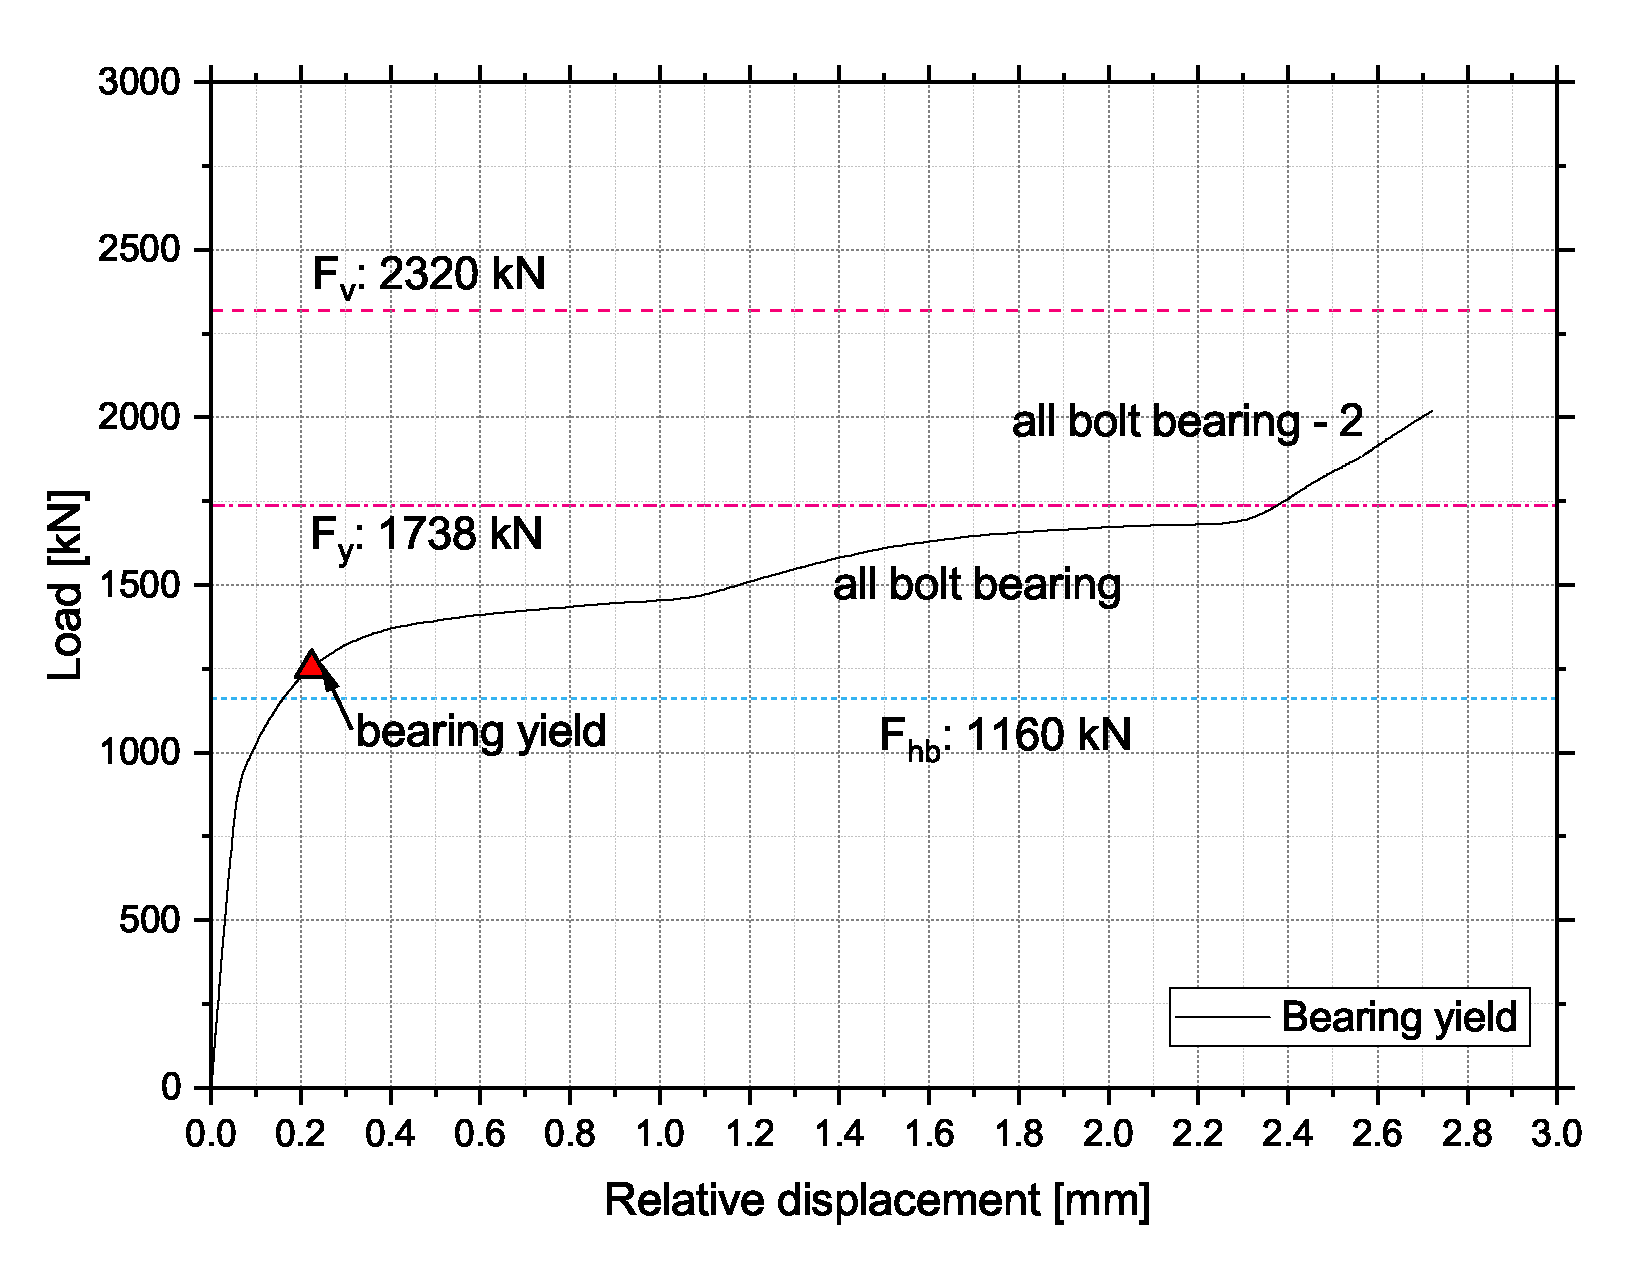
\includegraphics[width=0.7\textwidth]{imgs/ch7/b4s40t30.eps}
    \caption{The relationship between load and relative displacement for bearing yield first case.}
    \label{fig-beafst}
\end{figure}

Fig. \ref{fig-beafstcp} shows the Mises stress counter of the joint for bolts (thickness center of main plate, Maximum = 900 Mpa, when load = 1251 kN), Fig. \ref{fig-beafstcp-2} shows the Mises stress counter of the joint for the main plate (faying surface of the main plate, Maximum stress = 235 Mpa, when load = 1251 kN), From the figure, it can be found that when the load is equal to 1251 kN, the whole cross-section within the bearing contact range of the main plate has yielded, and it can be assumed that the joint has yielded under pressure, and at this time, the joint is in the limit state of yielding under pressure, and with reference to Fig. \ref{fig-beafst}, it can be found that the curve is experiencing a nonlinear change at this time, and it is about to enter into the stage of plastic ductility.

Fig. \ref{fig-beafstcp} shows the Mises stress counter of the joint for the plate (thickness center of main plate, Maximum stress = 900 Mpa, when load = 1251 kN). Against Fig. \ref{fig-beafst}, it can be seen from this figure that it is not the yielding of the shear plane of the bolt that causes the curve to go into a nonlinear behavior, so this state can be ruled out.

\begin{figure}[htbp]
    \centering
    \begin{minipage}[t]{0.8\textwidth}
    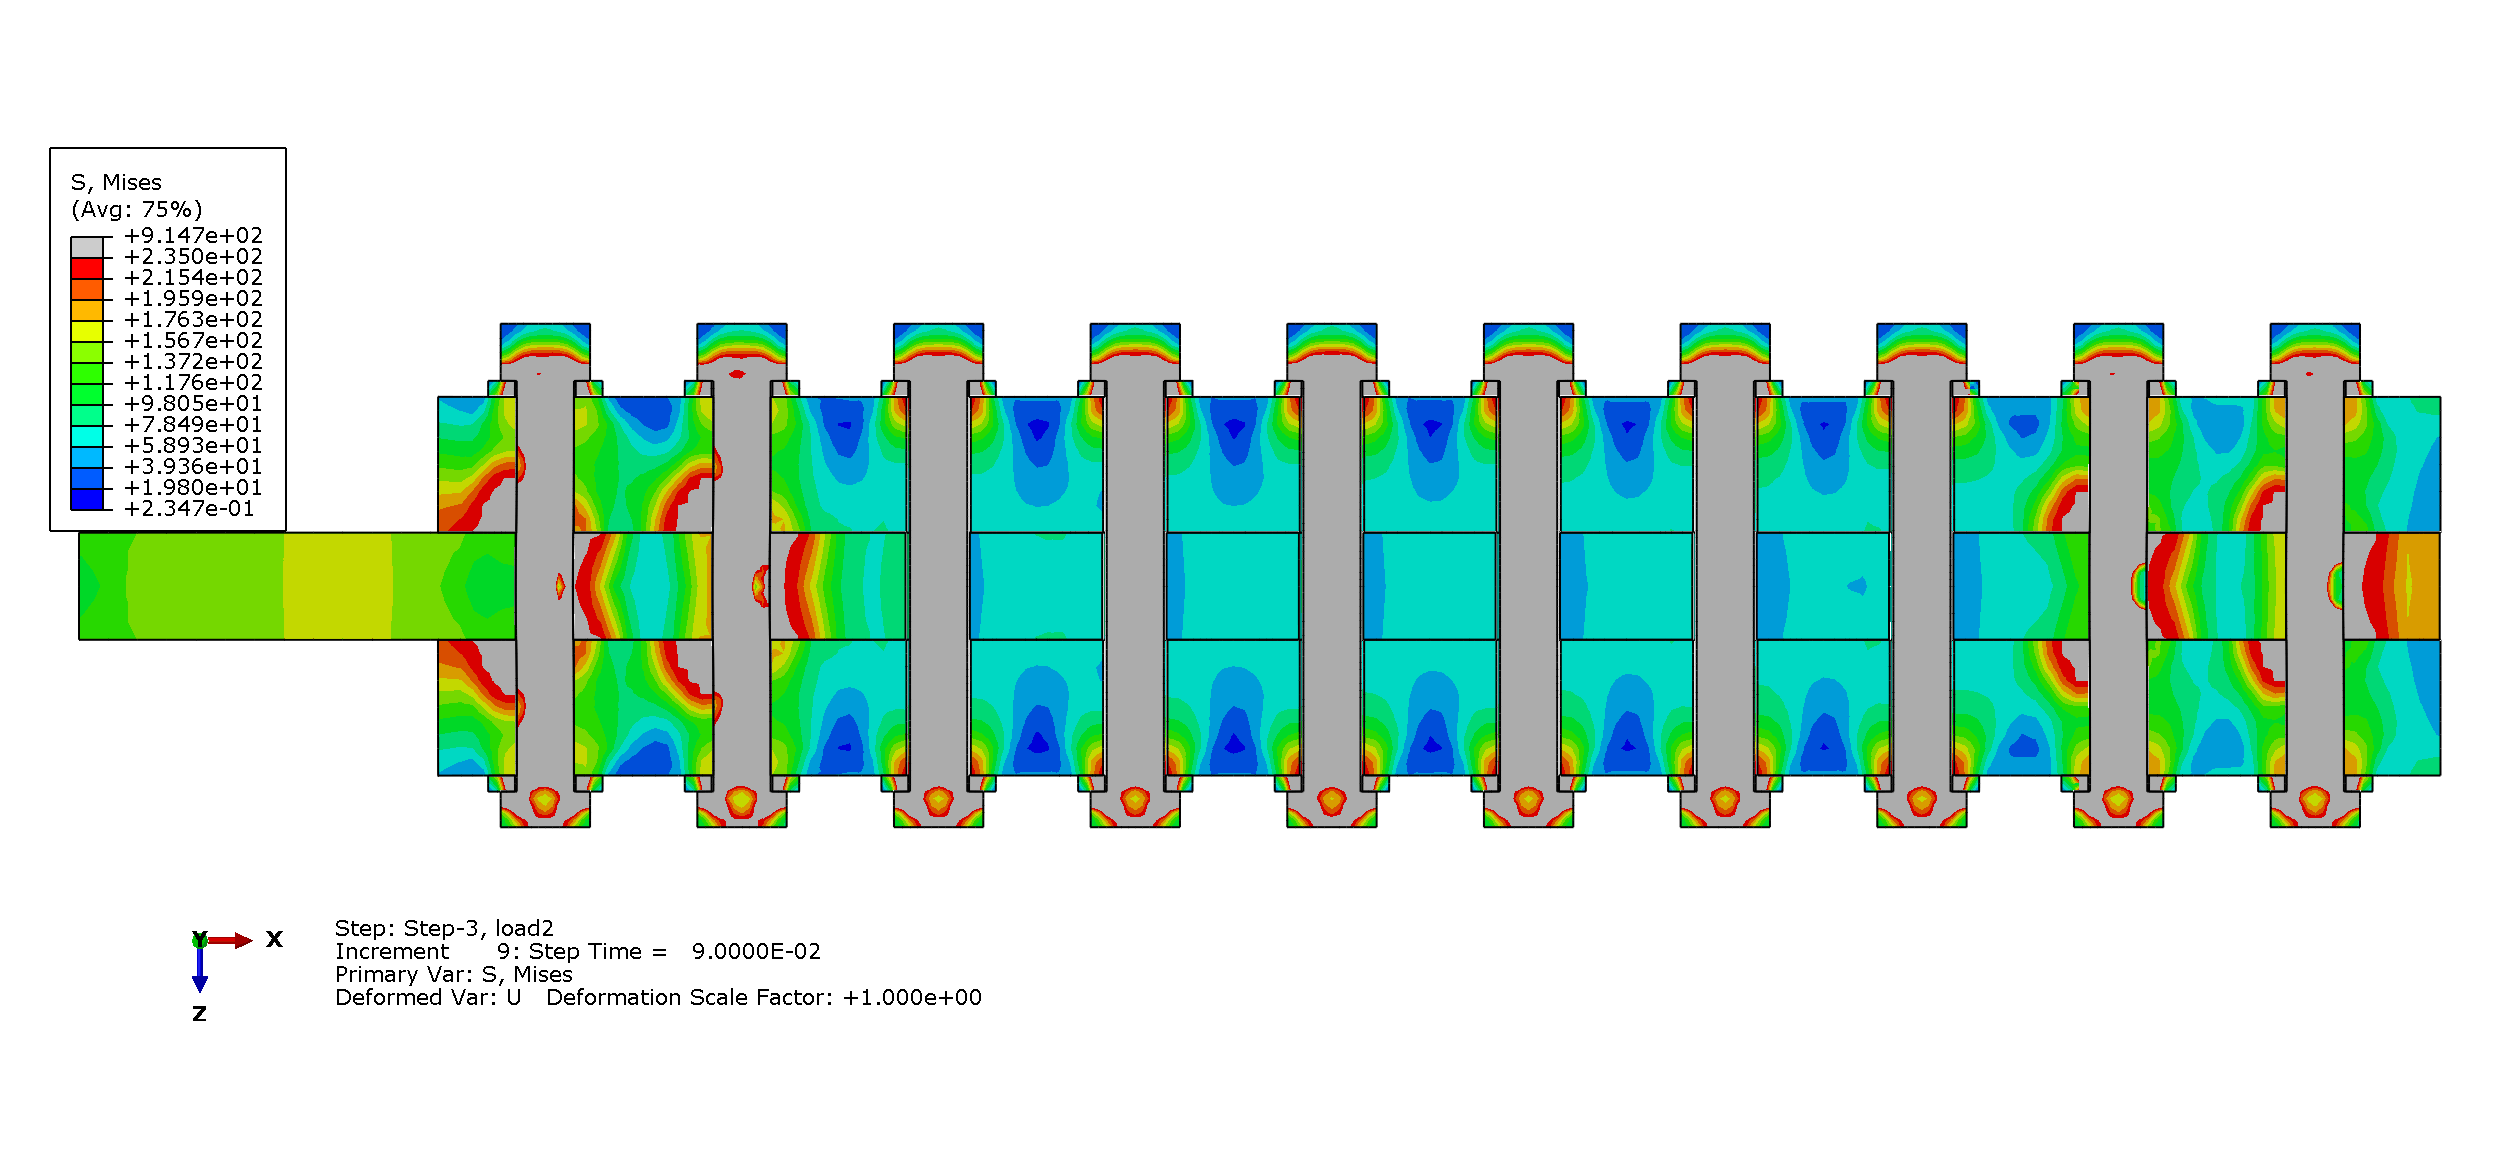
\includegraphics[width=\linewidth]{imgs/ch7/beafst-count-p.png}
    \caption{Mises stress counter of the joint for bolts (thickness center of main plate, Maximum stress = 235 Mpa, when load = 1251 kN)}
    \label{fig-beafstcp}
    \end{minipage}
    \begin{minipage}[t]{0.8\textwidth}
    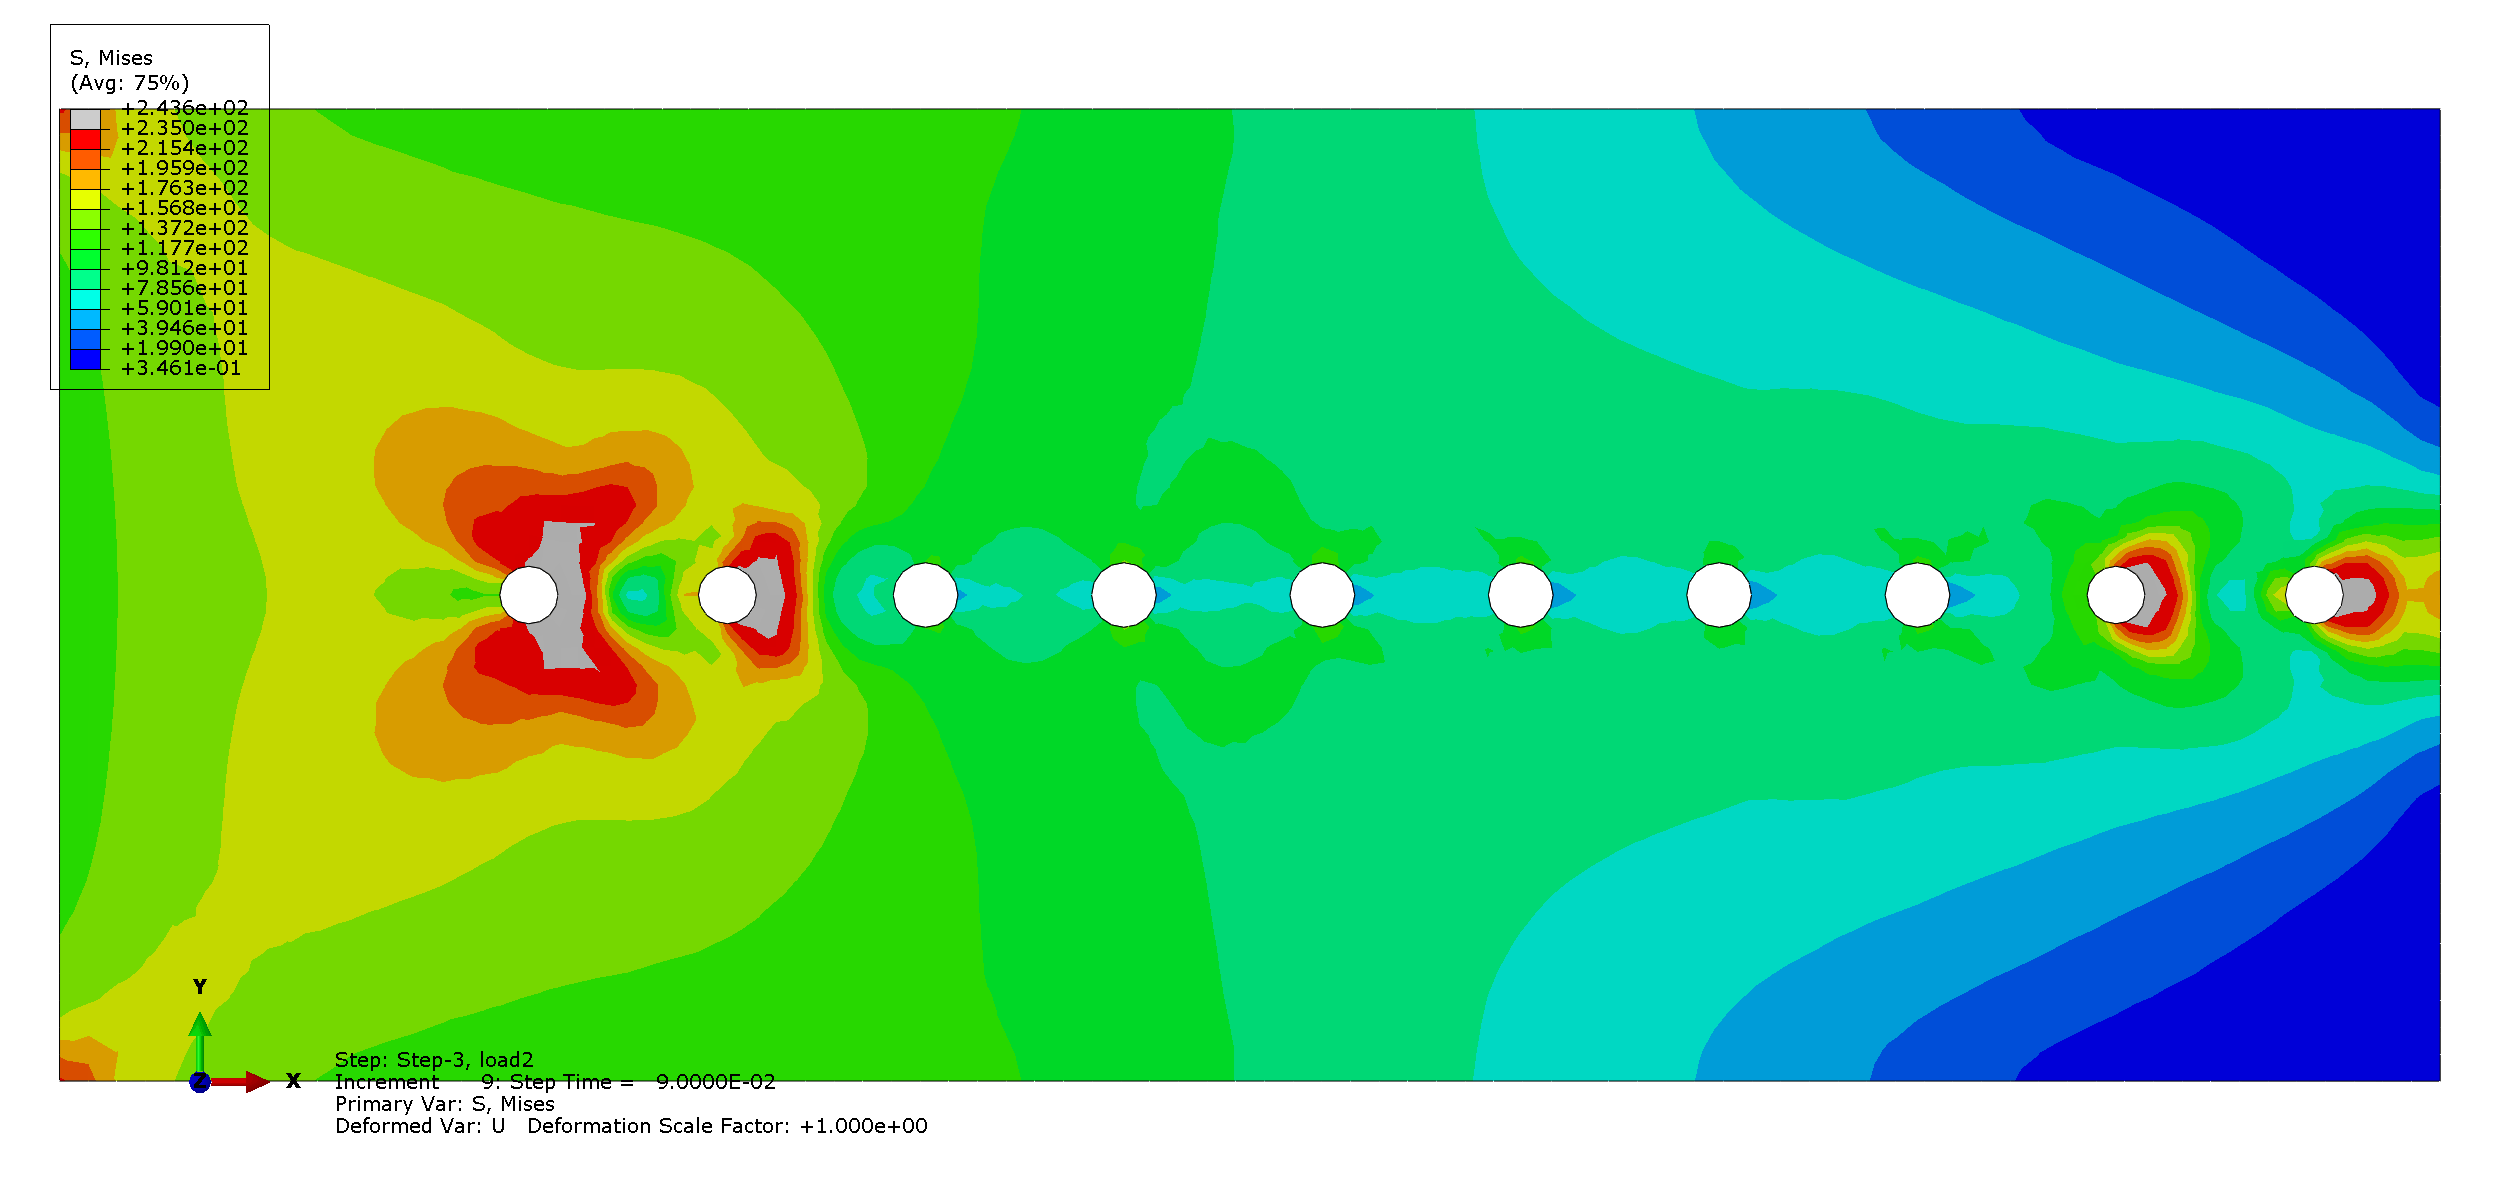
\includegraphics[width=\linewidth]{imgs/ch7/beafst-scout-mp.png}
    \caption{Mises stress counter of the joint for the main plate (faying surface of the main plate, Maximum stress = 235 Mpa, when load = 1251 kN)}
    \label{fig-beafstcp-2}
    \end{minipage}
    \begin{minipage}[t]{0.8\textwidth}
    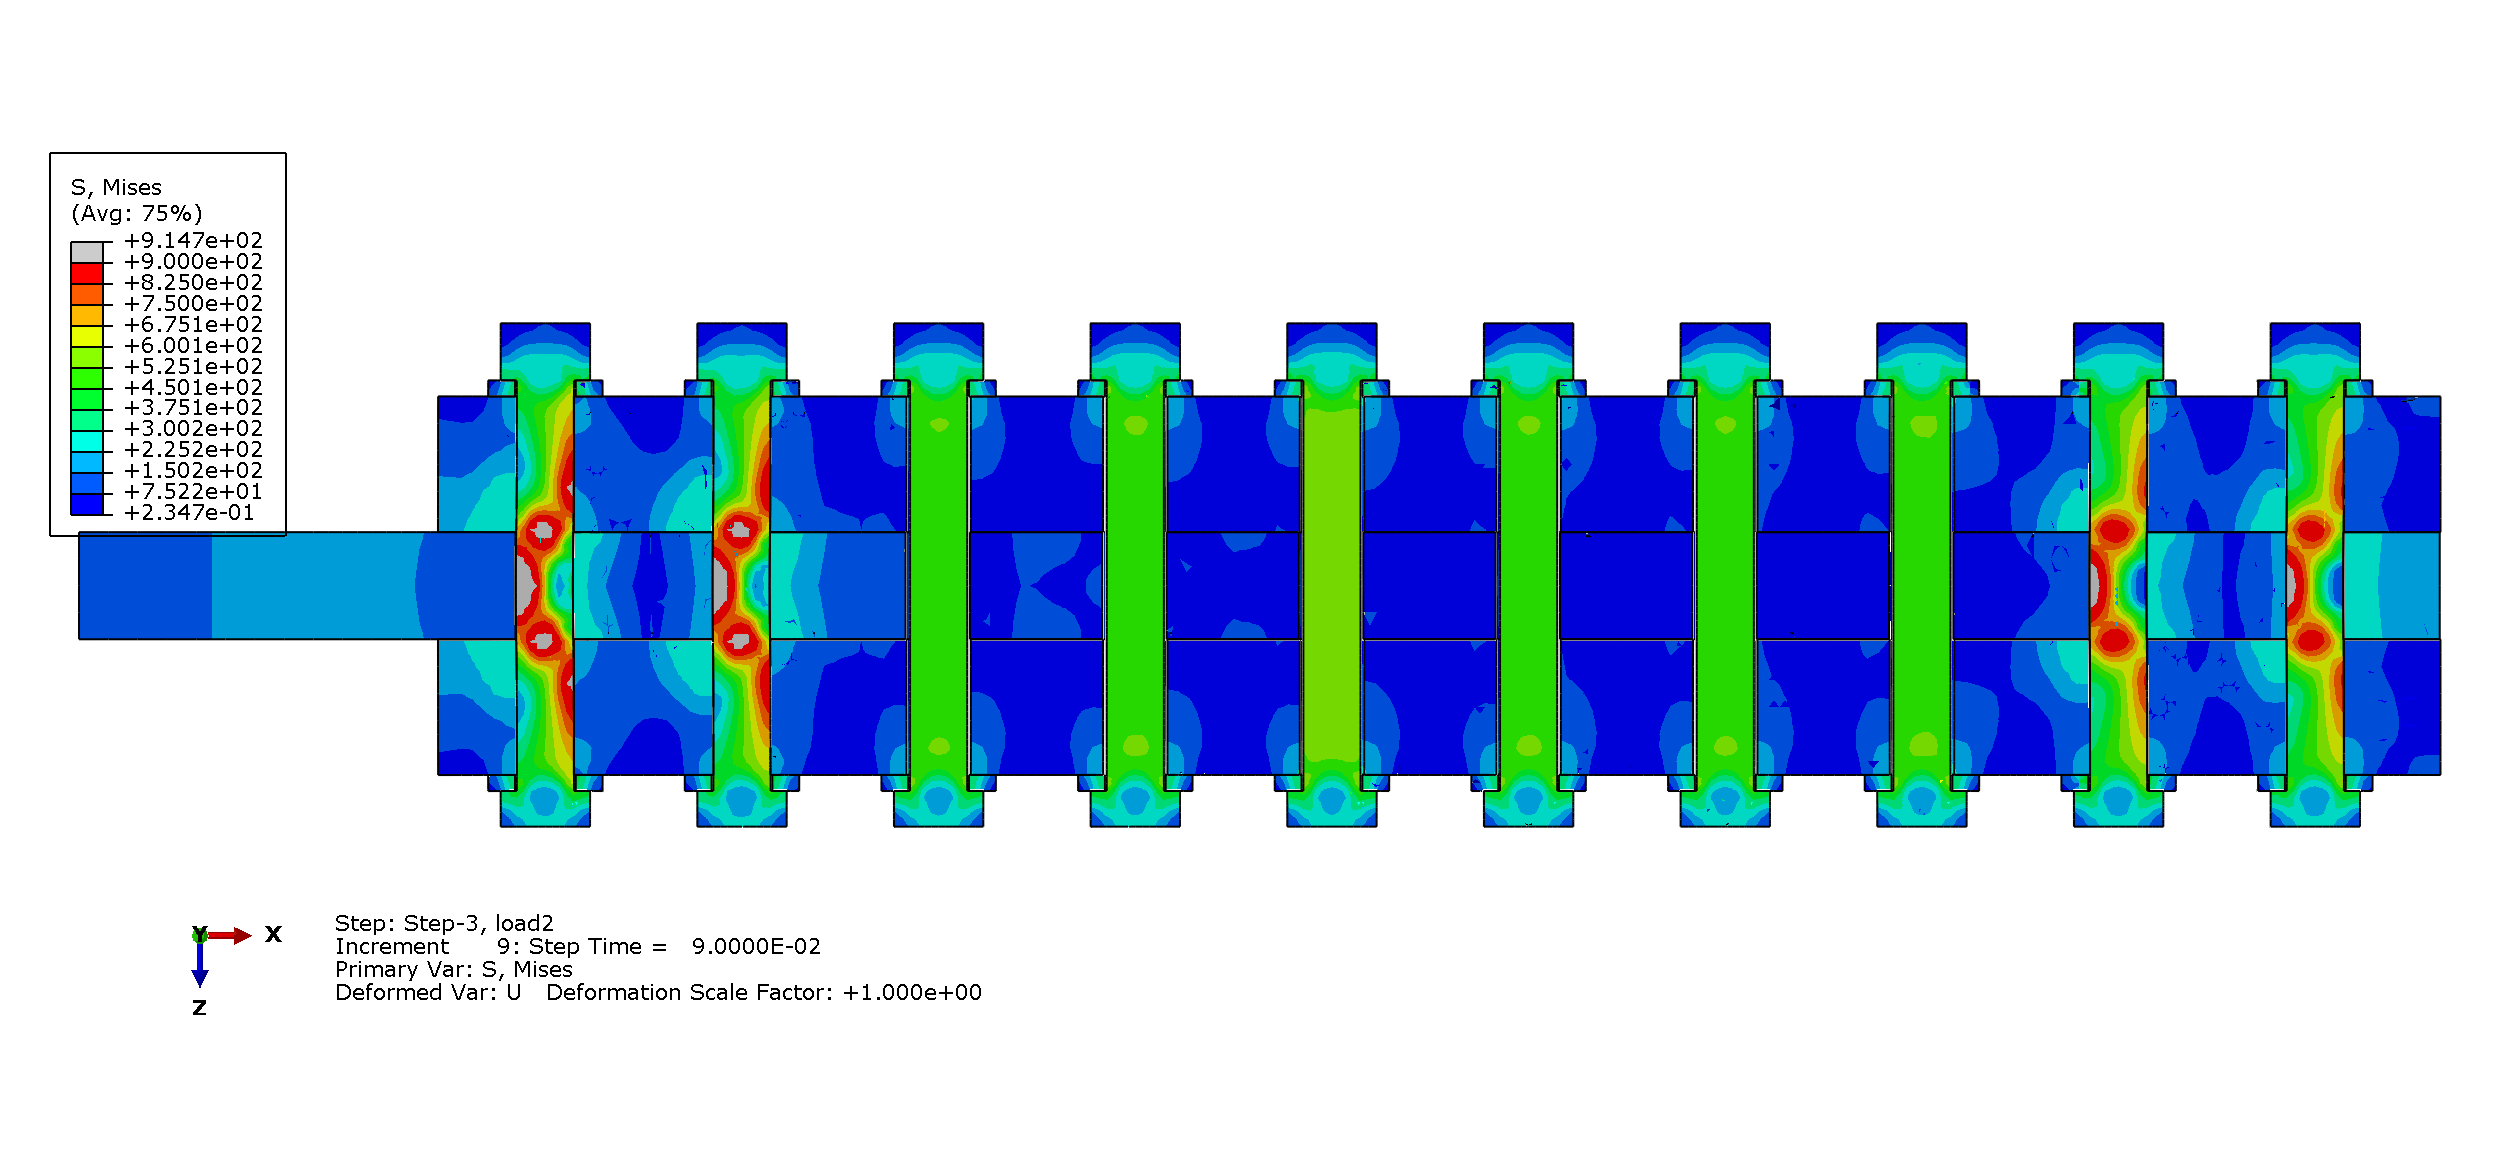
\includegraphics[width=\linewidth]{imgs/ch7/beafst-count-b.png}
    \caption{Mises stress counter of the joint for the plate (thickness center of main plate, Maximum stress = 900 Mpa, when load = 1251 kN)}
    \label{fig-beafstcb}
    \end{minipage}
    \label{fig-beafstc}
\end{figure}



\subsubsection{Reduction factor}

Fig. \ref{fig-beafstls} shows the Decline ratio of bolt preload when load is equal to the 1251 kN (bearing yield first case). From the figure, it can be seen that when it is judged as bearing yielding, since the nonlinear behavior of the joint arises around the bolt holes of the main plate, there is not much effect on the shaft of the bolt, and the bolt shaft as a whole is still in the linear elasticity stage, so the preload of the bolt does not change significantly as in the case of shear yielding case. Although the preload still drops to about 0.9, this value is very small for the whole, so it is considered here that the correction factor for the slip strength regarding the preload can be disregarded for the bearing resistance yield case.

\begin{figure}[htbp]
    \centering
    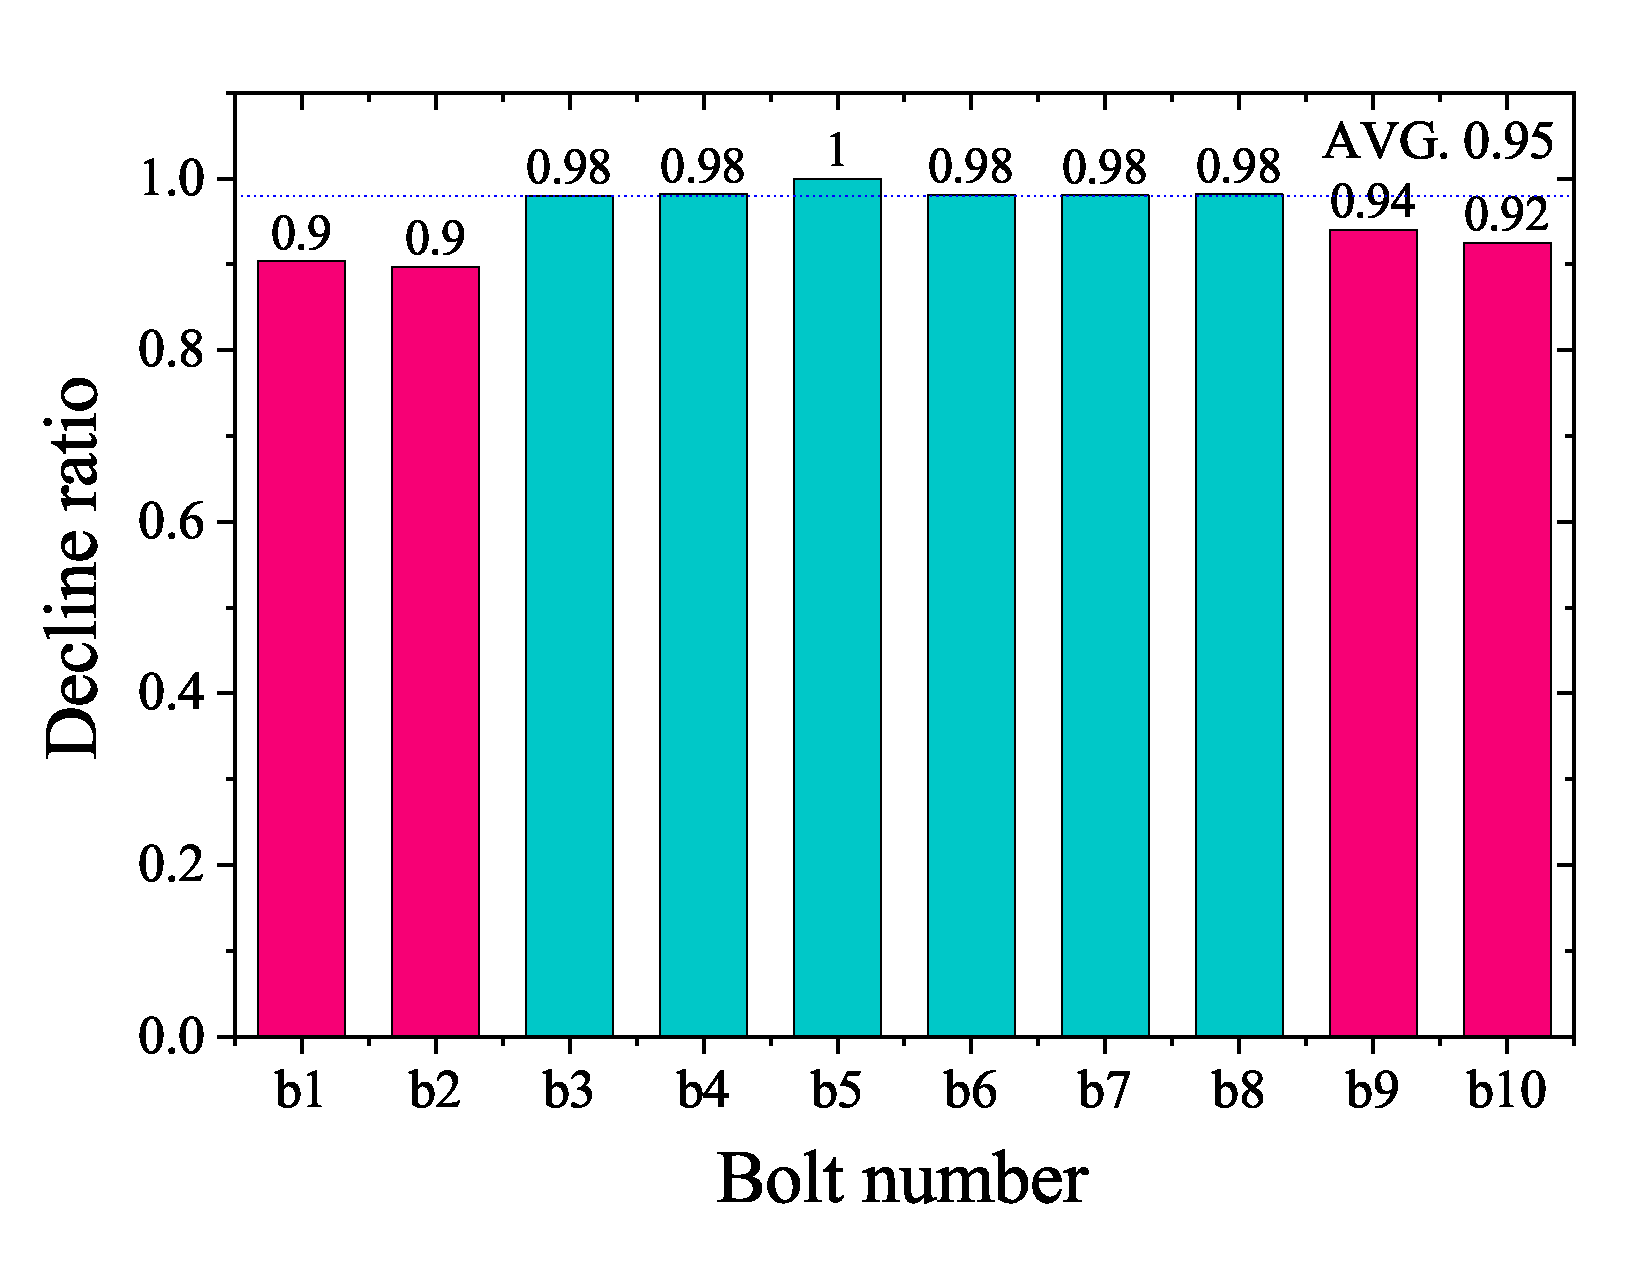
\includegraphics[width=0.7\textwidth]{imgs/ch7/b4t30w27-ls.eps}
    \caption{Decline ratio of bolt preload when load is equal to the 1251 kN (bearing yield first case)}
    \label{fig-beafstls}
\end{figure}


\subsubsection{Summary}

For the bearing yield limit state, since the occurrence of nonlinear behavior depends around the main plate fastener holes, the fasteners used for bearing connections are also not subjected to excessive shear resulting in a loss of preload, however, like the shear yield mode, the friction located in the if the front end is configured with a fastener used for a bearing type of connection, which produces a moment due to shear, will cause the main plate to deform and will still result in a friction force Therefore, it is not recommended to take into account the friction of bolt (b1) at the front end for such cases. The reduction factor due to the uneven distribution of loads in the bearing connection is still applicable to bearing resistance, therefore it is still recommended to multiply this reduction factor $\beta_{ls}$ when calculating the bearing yield resistance $F_{hv}$.

For SLS:
if bearing type connection is arranged at the front end of the joint :

\begin{equation}
\begin{aligned}
    F_{hb} &= (n-1) F_s + \beta_{ls} n_b F_{by1}\\
           &= (n-1) F_s + 0.9 n_b F_{by1}
\end{aligned}
\end{equation}

if not :

\begin{equation}
\begin{aligned}
    F_{hb} &= n F_s + \beta_{ls} n_b F_{by1}\\
           &= n F_s + 0.9 n_b F_{by1}
\end{aligned}
\end{equation}

For ULS, see other specifications such as Eurocode 3:

\begin{equation}
    F_v = n k_m \alpha_b d t f_{u}
\end{equation}


\subsection{Net cross-section yield}

For the net interfacial yield strength of the main slab, the method of calculation has not changed from the recommendations given in the various codes and is calculated according to the following equation.

\begin{equation}
    F_y = (w-d_0) t f_y
\end{equation}



\section{Conclusions}

For hybrid joints with friction and bearing connections, the service limit states can be categorized as: a.Shear yield limit state for the fastener shaft, b. Bearing yield limit state for main plate, c. Net cross-section yield limit state as shown in Fig. \ref{fig-schehysls}.

\begin{figure}[htbp]
    \centering
    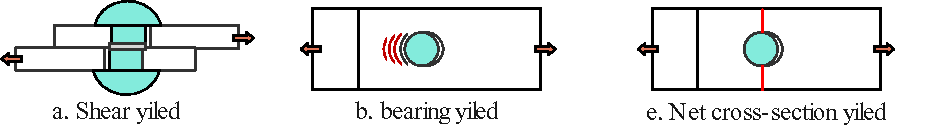
\includegraphics{imgs/ch7/sche-hy-sls.pdf}
    \caption{Schematic of the yield mode on the serviceability limit state}
    \label{fig-schehysls}
\end{figure}

Table\ref{tab-sumeq} summarizes the calculate equation for the hybrid joint on the serviceabilit limit state.

Hybrid joints mainly take into account the loss of preload due to shearing of the fasteners and the loss of friction of the fasteners located at the ends, in addition to the proposed discount factor due to the uneven distribution of loads in the bearing connection.

\begin{table}[htbp]
\centering
\caption{Calculate equation for hybrid joint on the SLS} \label{tab-sumeq}
\begin{tabular}{@{}lcc@{}}
\toprule
\multicolumn{3}{c}{Serviceability limit state}                                                  \\ \midrule
\multicolumn{1}{c}{} & \begin{tabular}[c]{@{}c@{}}If b1 arranged \\ fastener for bearing\end{tabular} & \begin{tabular}[c]{@{}c@{}}If \\ not\end{tabular} \\ \cmidrule(l){2-3} 
\begin{tabular}[c]{@{}l@{}}Shear yield resistance\\ for fastener shaft $F_{hv}$\end{tabular} &$(n_f+ \alpha_v(n_b-1)) F_s + \beta_{ls} n_b F_{vy1}$ & $(n_f+ \alpha_v n_b) F_s + \beta_{ls} n_b F_{vy1}$ \\
\begin{tabular}[c]{@{}l@{}}Bearing yield resistance\\ for main plate $F_{hb}$ \end{tabular}   & $(n-1) F_s + \beta_{ls} n_b F_{by1}$ & $ n F_s + \beta_{ls} n_b F_{by1}$ \\
\begin{tabular}[c]{@{}l@{}}Net cross-section yield\\ resistance $F_y$\end{tabular}   & \multicolumn{2}{c}{$ (w-d_0) t f_y$} \\ \bottomrule
\end{tabular}
\end{table}

Where, $\alpha_v$ is Correction factor for loss of preload due to shear failure, $\beta_{ls}$ is the correction factor for load sharing. $n$ is the number of the fastener, $n_f$ is the number of the fastener for friction type connections, $n_b$ is the number of the fastener for bearing type connections, $F_{by1}= dtf_y$, $F_{vy1} = A_s f_{yb}/\sqrt{3}$.

In addition, the reduction factor due to the conversion of static friction to kinetic friction should also be considered. However, the loading rate required for the conversion of static friction to kinetic friction varies according to the joint processing conditions, so in order to simplify the calculations, the friction coefficient can be considered as a factor of slip instead of slip coefficient for calculating the slip strength, and this topic will be discussed in the future to calculate the reliability of the calculation based on the coefficient of friction.

For the limit states, it is considered sufficient to follow the existing methods of strength calculation and classification. The only difference is that since all fasteners do not enter the bearing connection at the same time, fasteners that enter the bearing connection at the beginning may fail prematurely due to early entry into the bearing state, and therefore the strength of the limit states of the hybrid connection may be considered to require a reduction factor.


\subsubsection*{Deformation}

 In the case of the bolt shank shear yield limit state, the hybrid joints arranged with two and four fitted bolts (see Figure \ref{fig-loadrd-beaf}) produce almost the same relative displacements of approximately 0.4 $mm$ when the bolt shank shear yield strength $P_{h,sh}$ is reached. 
    
%ボルトシャンク全体せん断降伏限界状態の場合、2本の支圧型ボルト(図\ref{fig-ldoa2b}参照)と4本の支圧型ボルト(図\ref{fig-ldoa2b}参照)を配したハイブリッド継手では、ボルトシャンク全体せん断降伏強度P_{h,sh}に達したときの相対変位はほぼ同じ0.43mmとなる。これは、ボルトがせん断面で降伏したときに生じる弾性変形量が同じであることによると考えられる。従って、判定条件をボルトシャンクのせん断降伏強度時の荷重とすれば、そのボルトで生じる弾性変形量は同一と仮定できる。

Although the relative displacement at E-10mm (the location 10 mm away from the inner side of the joint, see Figure \ref{rd-distri}) was approximately 0.4 mm when the hybrid joint was in SLS, the relative displacement distribution of the long hybrid joint is significantly uneven, with an overall mean of 0.24 mm and a median of 0.2 mm.
    

\subsubsection*{Load sharing}

The fit bolts exhibit varying degrees of friction force degradation due to the different load transfer mechanisms of the bearing and friction, with the frontmost \# 1 bolt experiencing the most severe reduction. When four fitted bolts are used (two at each end), uneven bearing load distribution arises. Although the second \# 2 bolt appears to share a higher load, the frontmost \# 1 bolt relies almost entirely on the bearing to transfer the load due to the loss of friction force, resulting in the highest bearing force among all fitted bolts and leading to its bolt shank shear yielding first. Moreover, the uneven bearing load distribution prevents the bearing resistance from reaching the design bearing strength.

%長いすべり型継手の場合、荷重分布の偏りにより中央のボルトが許容すべり値を超えて設計すべり強度に達することができず、日本の道路橋示方書によってすべり耐力の低減係数が提案されている。一方、ハイブリッド継手では、すべり型継手の中央ボルトでは一様な荷重分担が生じ、設計すべり耐力に達する。一方、支圧型のボルトでは支圧伝達機構のため種々の程度の摩擦力劣化が生じ、最前列の#1ボルトで最も厳しい低減が生じる。4本の支圧型ボルト(各端部2本)を使用する場合、支圧荷重分布の偏りが生じる。#2ボルトが比較的高い荷重を分担するように見えるが、#1ボルトはほとんど全荷重を支圧で伝達せざるを得ず、摩擦力を失っているため、全支圧型ボルトの中で最大の支圧力が作用し、これがボルトシャンクの全体耐力に先行して降伏する。さらに、支圧荷重の偏り分布により、支圧耐力が設計支圧強度に達することができない。


\subsubsection*{Interaction of bearing and friction}

The cross-sectional force acting on the main plate is divided into forces on the main and splice plates via bolt shear transfer, generating an additional bending moment in the bolt due to the eccentricity of these forces. The shear bending of the fit bolt causes a severe loss of preload, resulting in a significant reduction in the frictional force it can transmit.

In addition, this bending moment causes the free end of the splice plate to deform outwards from the main plate, with a relative displacement of 0.43 mm at E-10mm and a maximum out-of-plane deformation of 0.07 mm at the end when the connection reaches bolt shank shear yield, resulting in separation and a loss of friction force. 

During Stage 1 of the hybrid connection, the bearing connection experiences delayed loading (the bearing starts to transfer load after a certain amount of slip occurs). Additionally, since the uneven load distribution of the bearing force in the fit bolts and the loss of friction force in the front bolt \#1, bolt shank shear yield generally occurs first in the front bolt \#1, and the bearing force could not reach the strength corresponding to the number of bolts.

% %主板に作用する断面力は、ボルトのせん断伝達を介して主板と継手板の力に分配され、この力の偏心によりボルトに追加曲げモーメントが生じる。この曲げモーメントにより、継手板の自由端が主板の摩擦面から外側に変形し、離間と摩擦力の喪失が生じる。この追加曲げモーメントにより継手板は変形し、ボルトシャンク全体せん断降伏時にE-10mmで0.43mmの相対変位と、端部で0.07mmの最大面外変形が生じる。ボルトの圧縮側では、ボルト変形により高い接触圧が発生するが、全体として摩擦面の接触圧は低下傾向にある。


% %在混合阶段处于stage-1时,由于摩擦的高刚性,承压连接会出现延迟受力(承压会在产生一定的滑移量之后开始传递载荷),且由于fit螺栓承压力的载荷分担不均匀,以及前端 \# 1螺栓的摩擦力损失,螺栓剪切屈服一般会发生在前端的\# 1螺栓,承压力达不到螺栓数量的强度。
% %ハイブリッド継手の第1段階では、摩擦の高い剛性により、支圧継手部の荷重伝達が遅延する(すべりが生じた後に支圧荷重が伝達され始める)。加えて、支圧型ボルトの支圧力分布の偏りと最前列ボルト#1の摩擦力喪失により、通常、最前列ボルト#1でボルトシャンク全体せん断降伏が先行し、ボルト本数分の支圧強度に到達できない。

%\end{itemize}

\subsubsection*{Reduction factor of bearing and friction}


%本文提出在计算混合连接剪切屈服强度时,分别对摩擦力和承压力进行折减,可以通过公式20计算其强度。其中摩擦力的折减系数参考公式21,配置两根和4根fit螺栓的情况分别取不同的折减系数,而关于承压力的折减系数,由于其偏差较小,因此取此次解析结果的下99%CI值作为折减系数,为0.76(统计结果可以参考表1). 通过公式20校正后的计算结果与解析值也较为吻合(见图19-c)。
This study proposes separately reducing the friction force and bearing force when calculating the bolt shank shear yielding strength of a hybrid connection, and its strength can be calculated using Eq. \ref{eq-pvh-2}. For the reduction factor of the friction force, refer to Eq. \ref{eq-as}, where different reduction factors are taken for the cases with two and four fitted bolts. As for the reduction factor of the bearing force, since its deviation is small, the lower 99\% CI of 0.76 from the analysis results in this study is taken as the reduction factor (the statistical results are listed in Table \ref{tab-rdfactor}). After correction using Eq. \ref{eq-pvh-2}, the calculated results match well with the analytical values (see Figure \ref{fig-fhv-cor2}).